\chapter{Search for nonresonant HH production in the bb\texorpdfstring{$\tau\tau$}{ττ} final state}
\label{ch:bbtt_analysis}
% Entradilla
Among the channels available for the production of Higgs boson pairs at the LHC, the final state in which one of the Higgs bosons decays into a pair of $b$ quarks and the other into a pair of $\tau$ leptons holds a privileged position, since it offers a favorable trade-off between the expected number of signal events and the accompanying background. Consequently, it is one of the channels most systematically explored in the successive searches conducted by CMS. 

The experimental signature of this process is not unique, since the $\tau$ lepton is unstable, which gives rise to different reconstructible final states resulting from the $\tau\tau$ pair. As listed in Table \ref{tab:tau_decays}, the $\tau$ lepton decays predominantly into hadrons and a neutrino, with a total branching fraction of $64.8\%$, and leptonically into an electron or a muon accompanied by two neutrinos, with branching fractions of $17.8\%$ and $17.4\%$ respectively, denoted $\tau_h$, $\tau_e$, and $\tau_\mu$ correspondingly. Only the three pairings in which at least one $\tau$ decays hadronically are considered signal channels, since they provide a favorable balance between signal branching fraction, reconstruction efficiency and background rejection: the fully hadronic $\tau_h\tau_h$ and the semileptonic $\tau_\mu\tau_h$ and $\tau_e\tau_h$, which together account for $87.6\%$ of the total branching fraction. Apart from the channels in which the signal is expected, the purely leptonic pairings, which have a smaller branching fraction, are used in the analysis as control regions since they are overwhelmed by background production.

The analysis presented in this chapter describes the strategy followed in the search for non-resonant production of Higgs boson pairs in this final state, considering the two relevant production mechanisms: gluon-gluon fusion, sensitive to the trilinear self-coupling $\lambda_{HHH}$ via interference between triangle and box diagrams, and vector boson fusion, which provides complementary sensitivity to the coupling of two Higgs bosons to two vector bosons, $\lambda_{2V}$. The analysis is performed using proton-proton collision data collected by CMS during the first years of LHC Run 3 — 2022, 2023, and 2024 — corresponding to an integrated luminosity of $172$ fb$^{-1}$. The search presented here builds on the work carried out on the complete Run 2 dataset~\cite{CMS-HIG-20-010}, but introduces significant developments that take advantage of the Run 3 improvements at various levels. 

The strategy therefore keeps the structure of the Run 2 search, with the three resolved channels defined by the decay of the $\tau\tau$ pair, the reconstruction of the two Higgs boson candidates and the general signal extraction scheme, but revises virtually every step. The phase space is extended to boosted configurations of both the $b\bar{b}$ and the $\tau\tau$ pairs, the latter through a fourth signal channel dedicated to boosted $\tau_h\tau_h$, and the trigger strategy incorporates new triggers, including parking streams that allow lower thresholds. The assignment of jets to the reconstructed candidates relies on the two algorithms developed in the previous chapter: \textsc{HH-BTag}, retrained for Run 3 conditions, and \textsc{VBFjTag}, introduced here for the first time in an analysis of this final state. Furthermore, a new method is developed for estimating the contribution of jets misidentified as $\tau_h$, extended from multijet production to all three processes that contribute to it, as well as a new DNN for signal extraction in different regions.


The complete analysis workflow is represented in Figure \ref{fig:bbtt_flow}, which serves as a roadmap for the following chapters. Following the analysis workflow, the data collected by CMS and the MC simulated events undergo the same trigger selection, designed to isolate the objects of interest. Identification criteria and kinematic requirements that define the physical objects in the final state are then applied to the events that pass this selection. From these events, the Higgs boson candidate that decays into the $\tau\tau$ pair, the one that decays into the $b\bar{b}$ pair, and — when present — the jets characteristic of VBF topology, are successively reconstructed. A selection based on the reconstructed invariant masses removes the region lacking signal contribution, and the surviving events are divided into mutually exclusive categories. In each category, the discrimination between signal and background is performed by a DNN whose output distribution constitutes the observable on which the statistical fitting is performed, from which the results are extracted.
%
\begin{figure}[tp]
\centering
\definecolor{smpBg}{HTML}{EEF3FB}\definecolor{smpLn}{HTML}{8FB0DC}
\definecolor{trgBg}{HTML}{F2EFF9}\definecolor{trgLn}{HTML}{A897D3}
\definecolor{objBg}{HTML}{FBF0F4}\definecolor{objLn}{HTML}{D79BB0}
\definecolor{selBg}{HTML}{FBF4EA}\definecolor{selLn}{HTML}{D6AE7C}
\definecolor{bkgBg}{HTML}{EFF6ED}\definecolor{bkgLn}{HTML}{92BF8C}
\definecolor{extBg}{HTML}{ECF7F5}\definecolor{extLn}{HTML}{72B9B1}
\definecolor{staBg}{HTML}{EFF1F5}\definecolor{staLn}{HTML}{9AA4B8}
\definecolor{outBg}{HTML}{F2F2F4}\definecolor{outLn}{HTML}{AEAEB8}
\newcommand{\ffont}{\fontfamily{Nunito-TLF}\selectfont}
% band: #1 top, #2 bottom, #3 colour prefix, #4 title, #5 section references
\newcommand{\band}[5]{%
  \fill[#3Bg, rounded corners=5pt] (0,#1) rectangle (158,#2);
  \draw[#3Ln, line width=0.6pt, rounded corners=5pt] (0,#1) rectangle (158,#2);
  \fill[#3Ln, rounded corners=5pt] (0,#1) rectangle (8,#2);
  \fill[#3Ln] (4,#1) rectangle (8,#2);
  \node[rotate=90, text=white, font=\ffont\tiny\bfseries, align=center, inner sep=0pt] at (4,{(#1+#2)/2}) {#4};
  \node[anchor=north east, align=right, font=\ffont\scriptsize\bfseries, text=#3Ln!75!black, inner sep=0pt] at (156.5,{#1-1.8}) {#5};
}
\begin{tikzpicture}[
    x=1mm, y=1mm, font=\ffont\footnotesize,
    cell/.style = {draw=#1, line width=0.5pt, fill=white, rounded corners=3pt,
                   align=center, inner sep=1.5pt},
    txt/.style  = {font=\ffont\scriptsize},
    res/.style  = {draw=outLn, line width=0.6pt, fill=outBg, rounded corners=3pt,
                   align=center, inner sep=1.5pt, font=\ffont\footnotesize\bfseries},
    hdr/.style  = {font=\ffont\footnotesize\bfseries\boldmath, text=#1!75!black, inner sep=0pt},
    lab/.style  = {anchor=west, font=\ffont\footnotesize\itshape, text=black!65, inner sep=0pt},
    ar/.style   = {-{Latex[length=1.8mm]}, draw=#1, line width=0.6pt}
  ]
  % ===================== SAMPLES
  \band{0}{-21.5}{smp}{SAMPLES}{\ref{sec:bbtt_samples}}
  \node[lab] at (12,-4.5)  {data};
  \node[lab] at (12,-11)   {signal};
  \node[lab] at (12,-17.5) {background};
  \node[cell=smpLn, minimum width=116mm, minimum height=5.2mm] at (88,-4.5)
      {CMS Run 3 \quad 2022\,--\,2024 \quad 172 fb$^{-1}$ \quad 13.6\,TeV};
  \node[cell=smpLn, minimum width=56mm, minimum height=5.2mm] at (58,-11)  {gluon fusion HH};
  \node[cell=smpLn, minimum width=56mm, minimum height=5.2mm] at (118,-11) {vector boson fusion HH};
  \foreach \x/\t in {38.75/{\textbf{Drell--Yan}}, 58.45/{{\boldmath\bfseries $t\bar{t}$}}, 78.15/{$W$\,+\,jets},
                     97.85/{single $t$}, 117.55/{single $H$}, 137.25/{multiboson}}
    \node[cell=smpLn, minimum width=17.5mm, minimum height=5.2mm] at (\x,-17.5) {\t};
  % ===================== TRIGGERS
  \band{-24}{-49}{trg}{TRIGGERS}{\ref{sec:triggers}}
  \foreach \x/\t in {24.4/single lepton, 51.7/lepton\,+\,$\tau_h$, 79.0/$\tau_h$ and jets,
                     106.3/VBF, 133.6/boosted}
    \node[hdr=trgLn] at (\x,-28) {\t};
  \foreach \x/\y/\t/\s in {24.4/-33.5/{single $\mu$}/solid, 24.4/-39.5/{single $e$}/solid,
                           51.7/-33.5/{$\mu+\tau_h$}/solid, 51.7/-39.5/{$e+\tau_h$}/solid,
                           79.0/-33.5/{DiTau}/solid, 79.0/-39.5/{DiTau\,+\,jet}/solid, 79.0/-45.5/{QuadJet}/dashed,
                           106.3/-33.5/{VBF\,+\,DiTau}/solid, 106.3/-39.5/{VBF\,+\,$\mu$, $e$, $\tau_h$}/dashed, 106.3/-45.5/{VBF inclusive}/dashed,
                           133.6/-33.5/{missing $p_T$}/solid, 133.6/-39.5/{large-radius jet}/solid}
    \node[cell=trgLn, \s, minimum width=24.8mm, minimum height=4.8mm] at (\x,\y) {\t};
  \node[font=\ffont\scriptsize\itshape, text=black!60, anchor=south east, inner sep=0pt] at (156.5,-48) {dashed: parking};
  % ===================== OBJECTS
  \band{-51.5}{-70.5}{obj}{OBJECTS}{\ref{sec:bbtt_objects}}
  \node[hdr=objLn] at (44.75,-55.5)  {leptons};
  \node[hdr=objLn] at (113.25,-55.5) {jets and missing $p_T$};
  \node[cell=objLn, txt, minimum width=65.5mm, text width=62mm, minimum height=10.5mm] at (44.75,-63)
      {identification, isolation and kinematic selections\\
       DeepTau for $\tau_h$, also in the boosted regime\\ veto of additional leptons};
  \node[cell=objLn, txt, minimum width=65.5mm, text width=62mm, minimum height=10.5mm] at (113.25,-63)
      {small- and large-radius jets\\ $b$ tagging with ParticleNet and UParT\\ missing $p_T$ with PUPPI};
  % ===================== EVENT SELECTION
  \band{-73}{-98}{sel}{EVENT\\SELECTION}{\ref{sec:bbtt_flow}}
  \node[hdr=selLn] at (37,-77)  {{\boldmath$H\to\tau\tau$} candidate};
  \node[hdr=selLn] at (90,-77)  {{\boldmath$H\to b\bar{b}$} candidate};
  \node[hdr=selLn] at (132,-77) {VBF jet pair};
  \node[cell=selLn, txt, minimum width=50mm, text width=47mm, minimum height=8mm] at (37,-83.5)
      {$\tau_\mu\tau_h$ \enspace $\tau_e\tau_h$ \enspace
       $\tau_h\tau_h$ \enspace $b\tau_h\tau_h$\\
       mass from a regression network};
  \node[cell=selLn, txt, minimum width=50mm, text width=47mm, minimum height=8mm] at (90,-83.5)
      {resolved: HH-BTag\\ boosted: ParticleNet};
  \node[cell=selLn, txt, minimum width=28mm, text width=25mm, minimum height=8mm] at (132,-83.5)
      {VBFjTag};
  \foreach \x/\t/\n in {27.25/boosted/k1, 61.75/VBF/k2, 96.25/res2b/k3, 130.75/res1b/k4}
    \node[res, minimum width=30.5mm, minimum height=5.2mm] (\n) at (\x,-92.5) {\t};
  \draw[ar=selLn!80!black] (k1) -- (k2);
  \draw[ar=selLn!80!black] (k2) -- (k3);
  \draw[ar=selLn!80!black] (k3) -- (k4);
  % ===================== BACKGROUND
  \band{-100.5}{-117}{bkg}{BACKGROUND}{\ref{sec:bbtt_corrections}\\\ref{sec:bbtt_ff}\\\ref{sec:bbtt_controlplots}}
  \node[hdr=bkgLn] at (44.75,-104.5)  {genuine $\tau_h$};
  \node[hdr=bkgLn] at (113.25,-104.5) {jets misidentified as $\tau_h$};
  \node[cell=bkgLn, txt, minimum width=65.5mm, text width=62mm, minimum height=8mm] at (44.75,-111)
      {simulation, with dedicated corrections\\ for Drell--Yan and $t\bar{t}$};
  \node[cell=bkgLn, txt, minimum width=65.5mm, text width=62mm, minimum height=8mm] at (113.25,-111)
      {fake factors measured in QCD multijet,\\ $t\bar{t}$ and $W$\,+\,jets enriched regions};
  % ===================== SIGNAL EXTRACTION
  \band{-119.5}{-134.5}{ext}{SIGNAL\\EXTRACTION}{\ref{sec:bbtt_extraction}}
  \node[cell=extLn, txt, minimum width=134mm, text width=130mm, minimum height=8mm] at (79,-127)
      {deep neural networks targeting gluon fusion and vector boson fusion HH production,\\
       whose output constitutes the observable of the search};
  % ===================== STATISTICAL ANALYSIS
  \band{-137}{-155.5}{sta}{STATISTICAL\\ANALYSIS}{\ref{sec:bbtt_systematics}\\\ref{sec:bbtt_statistics}\\\ref{sec:bbtt_results}\\\ref{sec:bbtt_combination}}
  \foreach \x/\n/\t in {26.9/a1/{signal and background\\predictions}, 61.6/a2/{systematic\\uncertainties},
                        96.4/a3/{binned maximum-\\likelihood fit}, 131.1/a4/{limits on HH, $\kappa_\lambda$, $\kappa_{2V}$\\ Run 2 combination}}
    \node[cell=staLn, txt, minimum width=29.75mm, text width=28.5mm, minimum height=11.5mm] (\n) at (\x,-146.75) {\t};
  \draw[ar=staLn] (a1) -- (a2);
  \draw[ar=staLn] (a2) -- (a3);
  \draw[ar=staLn] (a3) -- (a4);
\end{tikzpicture}
\caption[Schematic of the $bb\tau\tau$ analysis chain]{Schematic representation of the analysis chain, with one band per stage, from the data and simulated samples to the statistical analysis. The sections in which each stage is described are indicated at the top right of the corresponding band, so that the figure also serves as an index of the analysis.}
\label{fig:bbtt_flow}
\end{figure}



In this chapter, Section \ref{sec:bbtt_samples} presents the data and the simulated samples, Section \ref{sec:triggers} the trigger strategy with which the events are recorded, and Section \ref{sec:bbtt_objects} the reconstruction and preselection of the physics objects from which the final state is built; Section \ref{sec:bbtt_flow} then defines the event selection and the categories into which the events are classified. Sections \ref{sec:bbtt_corrections} and \ref{sec:bbtt_ff} describe the corrections applied to the simulation and the estimation of the contribution from misidentified jets, and Section \ref{sec:bbtt_systematics} the uncertainties assigned to both. The resulting prediction is compared with the data in Section \ref{sec:bbtt_controlplots}, and Section \ref{sec:bbtt_extraction} builds the discriminant whose distribution constitutes the observable of the measurement. That measurement — the statistical procedure through which the prediction is fitted to the data, the constraints that follow on the production cross section and on the couplings of the Higgs boson, and the combination with the Run-2 data set — is the subject of Chapter \ref{ch:bbtt_results}.




\section{Data and simulated samples}
\label{sec:bbtt_samples}
The analysis is based on a comparison between the data recorded by CMS and the SM prediction for the processes that contribute to this final state. The prediction is derived from simulated MC samples, produced using state-of-the-art generators (Section \ref{subsec:pp_simulation}), which are used to model both the signal and the backgrounds. In all samples, the parton shower, hadronization and underlying event are simulated with \PYTHIA 8~\cite{Bierlich:2022pfr} with the CP5 tune~\cite{CMS:2019csb}, and the response of the CMS detector is modeled using \GEANT~\cite{GEANT4:2002zbu}, with pile-up interactions superimposed, and reconstructed in the same way as the data (Section \ref{sec:POR}). Furthermore, the MC-based background predictions are supplemented with corrections and calibrations derived from data. The only exception is the contribution from events in which a quark or gluon jet is misidentified as a hadronic $\tau$ lepton: generating enough such events is computationally prohibitive, and the misidentification rate is in any case not modeled with the required precision, being highly sensitive to detector effects. This contribution is therefore estimated directly from the data.

\subsection{Datasets and data-taking periods}
%
The analyzed data correspond to proton-proton collisions at $\sqrt{s} = 13.6$ TeV recorded by CMS with a bunch crossing interval of 25 ns during the years 2022, 2023, and 2024. Only events occurring during data-taking periods in which all subdetectors were operational and functioning correctly, as determined by the centralized certification procedure of the collaboration, are considered. The resulting available integrated luminosity amounts to $34.7$, $27.7$, and $110$ fb$^{-1}$ for 2022, 2023, and 2024, respectively, for a total of $172$ fb$^{-1}$.

The recorded events are distributed across primary datasets, which are defined by the trigger paths that lead to their storage, and are in turn subdivided into eras — identified by a letter — that delimit intervals with homogeneous data-acquisition conditions. This analysis uses the \texttt{Muon} and \texttt{EGamma} datasets, which contain events selected by the isolated lepton and lepton plus $\tau_h$ triggers; \texttt{Tau}, associated with the double $\tau_h$ triggers; \texttt{JetMET}, which provides access to events selected by triggers based on jets and missing transverse momentum; and the \texttt{ParkingHH} and \texttt{ParkingVBF} parking sets, introduced during Run 3 and described in Section \ref{sec:triggers}.

The detector conditions did not remain constant over the data taking. In 2022, a region of one of the endcaps of the electromagnetic calorimeter was lost, and in 2023, a region of the barrel pixel detector, so that each of these years is divided into two periods -- 2022preEE and 2022postEE, and 2023preBPix and 2023postBPix --, each described by a dedicated simulation campaign that reproduces its detector configuration. Events with jets in these regions are rejected, as are, in 2022postEE, electrons in the affected region of the calorimeter, and the affected regions are moreover treated in the same way in data and simulation. Table \ref{tab:datataking_periods} lists the five resulting periods along with their integrated luminosity and the incident that caused each division. Furthermore, the 2022 and 2023 data were reprocessed to incorporate the corrections and algorithms available from the latest simulation campaigns, ensuring that all five periods are analyzed using a homogeneous reconstruction chain. The analysis is performed independently for each of these five periods, and the results are combined in the final statistical fit.
%
\begin{table}[t]
\centering
\small
\begin{tabular}{llcl}
\toprule
Period & Eras & $\mathcal{L}_{\mathrm{int}}$ [fb$^{-1}$] & Detector condition motivating the split \\
\midrule
2022preEE    & C--D & 8.0   & \multirow{2}{5.2cm}{Loss of a region of the ECAL endcap (EE)} \\
2022postEE   & E--G & 26.7  & \\
\addlinespace
2023preBPix  & C    & 18.0  & \multirow{2}{5.2cm}{Loss of a region of the barrel pixel tracker (BPix)} \\
2023postBPix & D    & 9.7   & \\
\addlinespace
2024         & C--I & 109.8 & No incident \\
\midrule
Total        &      & 172.1 & \\
\bottomrule
\end{tabular}
\caption{Data-taking periods considered in the analysis, with the certified integrated luminosity of each one and the detector malfunction that motivates its separation.}
\label{tab:datataking_periods}
\end{table}


%\begin{figure}[t]
%  \centering
%  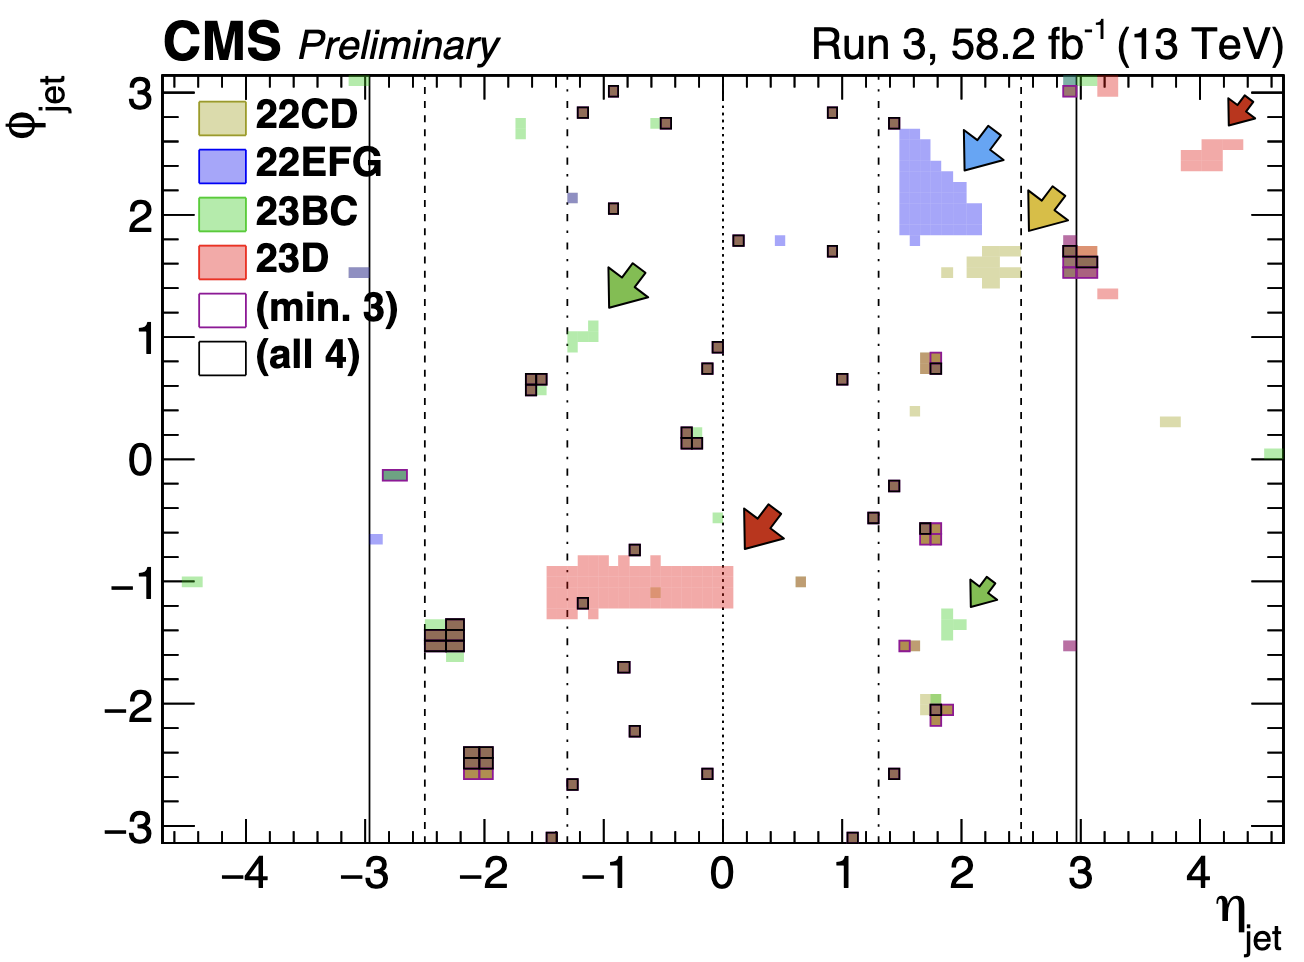
\includegraphics[width=0.8\linewidth]{figures/chapter_V/run3_detector_issues_etaphi.png}
%  \caption[Detector regions affected during the 2022 and 2023 data taking]{%    Regions of the CMS detector affected by an anomalous jet response during the 2022 and    2023 data taking, shown in the $\eta$--$\phi$ plane. The large blue area corresponds to    the region of the electromagnetic calorimeter endcap lost in 2022, and the large red band    to the region of the barrel pixel tracker affected in 2023. The remaining markings indicate    smaller areas of increased or decreased jet activity in the less affected eras; colors denote    the data-taking eras as given in the legend, and open boxes mark regions flagged in at least    three or in all four of them.}
%  \label{fig:detector_issues}
%\end{figure}


\subsection{Signal samples}
%
Higgs boson pair production via ggF is simulated using the \POWHEG v2.0 generator~\cite{powheg1,powheg2,powheg3} at NLO in QCD with full top quark mass dependence~\cite{Heinrich:2017kxx,Heinrich:2019bkc}, while the production via VBF is simulated using \MGaMC 2.9.13~\cite{Alwall:2014hca} at LO. The samples are normalized to the SM cross sections at $\sqrt{s} = 13.6$ TeV for a Higgs boson mass of $125$ GeV: $34.13$ fb for ggF, and $1.874$ fb for VBF. In both cases, additional samples are generated with anomalous values of the coupling modifiers (Section \ref{subsubsec:coupling_modifiers}), which make it possible to cover the dependence of the cross section and of the kinematics of the $HH$ system on these parameters.

Although optimized for the SM search, the analysis also constrains the coupling modifiers $\kappa_\lambda$ and $\kappa_{2V}$, which requires a prediction of the signal at any point of the coupling space. Simulating one sample per hypothesis is not feasible, but the polynomial dependence of the cross section on the couplings, Equations \ref{eq:kl_kt_ggf} and \ref{eq:vbf_poly}, which holds bin by bin for any distribution, allows the full dependence to be determined from as many samples as the polynomial has terms. For ggF, the three terms are obtained from the samples generated at $\kappa_\lambda = 1$, $2.45$ and $5$, with $\kappa_t = 1$, and for VBF, the six terms from those generated at $(\kappa_V, \kappa_{2V}, \kappa_\lambda) = (1, 1, 1)$, $(1, 0, 1)$, $(-0.962, 0.959, -1.43)$, $(-1.21, 1.94, -0.94)$, $(-1.60, 2.72, -1.36)$ and $(-1.83, 3.57, -3.39)$, six of the VBF points listed in Table \ref{tab:signal_points}.

Writing the polynomial at each of these points gives a linear system, $\vec{\sigma} = F\,\vec{a}$, where $\vec{\sigma}$ contains the cross sections of the samples, $\vec{a}$ the unknown coefficients, and each row of $F$ the monomials evaluated at one of the samples. Solving it and substituting the result back into the polynomial, the cross section at any other point $\boldsymbol{\kappa}$ is expressed as a linear combination of the simulated samples,
%
\begin{equation}
    \sigma(\boldsymbol{\kappa}) = \vec{f}^{\;\top}(\boldsymbol{\kappa})\, F^{-1}\,\vec{\sigma},
    \label{eq:matrix_inversion}
\end{equation}
%
where $\vec{f}(\boldsymbol{\kappa})$ is the vector of monomials evaluated at the target point. Since the decomposition holds bin by bin, the same combination is applied to the histograms of the final discriminant in every category, and the signal model is built in this way directly in the statistical fit.\medskip


This approach is known as the \textit{matrix inversion method}, and its general formalism, the conditions that the set of simulated points must satisfy for the inversion to be numerically stable, and its extension to the higher-dimensional parameter spaces of EFTs, are developed in Chapter \ref{ch:eft_modeling} as one of the original contributions of this thesis.








% ggHH: POWHEG v2 @ NLO. qqHH: MADGRAPH5_aMC@NLO 2.9.13 @ LO.
% Anomalous-coupling samples and the matrix-inversion reweighting that gives access
% to arbitrary (kappa_lambda, kappa_2V) -> forward-reference the EFT chapter.
% -> code: tasks/ggFReweightModules.py, tasks/VBFReweightModules.py

\subsection{Simulated background samples}
%
The SM processes that can reproduce the signature of the signal fall into two groups. Irreducible backgrounds lead to exactly the same final state, with two genuine $b$ quarks and two genuine $\tau$ leptons. The main one is top quark pair production, in which each top quark decays into a $b$ quark and a $W$ boson, and both $W$ bosons decay leptonically, either directly into an electron or a muon or through a $\tau$ lepton. It is followed by Drell--Yan production, $Z/\gamma^*\to\tau\tau$, when the lepton pair is accompanied by $b$ jets from gluon splitting. Single Higgs boson production also contributes despite its small cross section, in particular through $ZH$ production with $Z\to b\bar{b}$ and $H\to\tau\tau$. By contrast, reducible backgrounds only reproduce the final state when an object is misidentified: a light-flavor jet taken for a $b$ jet, an electron or a muon taken for a $\tau_h$ or, above all, a quark or gluon jet taken for a $\tau_h$. This is the case of QCD multijet production -- which dominates in the $\tau_h\tau_h$ channel --, of $W$ boson production in association with jets, and of the $t\bar{t}$ and Drell--Yan decays in which one of the objects of the final state is not genuine. Representative diagrams of the three main processes are shown in Figure \ref{fig:bkg_feynman}.
%
\begin{figure}[tbp]
    \centering
    \begin{fmffile}{bkgdiagrams}
    \begin{minipage}[b]{0.34\linewidth}
        \centering\small
        \begin{fmfgraph*}(100,72)
            \fmfleft{i1,i2}
            \fmfright{ob,ol2,on2,on1,ol1,ot}
            \fmf{gluon}{i1,va}
            \fmf{gluon}{i2,va}
            \fmf{gluon}{va,vb}
            \fmf{fermion,label=$t$,label.side=left}{vb,vt}
            \fmf{fermion,label=$\bar{t}$,label.side=left}{vtb,vb}
            \fmf{fermion}{vt,ot}
            \fmf{fermion}{ob,vtb}
            \fmf{photon,label=$W^+$,label.side=right}{vt,vw1}
            \fmf{photon,label=$W^-$,label.side=left}{vtb,vw2}
            \fmf{fermion}{ol1,vw1}
            \fmf{fermion}{vw1,on1}
            \fmf{fermion}{vw2,ol2}
            \fmf{fermion}{on2,vw2}
            \fmfforce{(0.0w,0.85h)}{i2}
            \fmfforce{(0.0w,0.15h)}{i1}
            \fmfforce{(0.2w,0.5h)}{va}
            \fmfforce{(0.4w,0.5h)}{vb}
            \fmfforce{(0.55w,0.8h)}{vt}
            \fmfforce{(0.55w,0.2h)}{vtb}
            \fmfforce{(0.8w,0.7h)}{vw1}
            \fmfforce{(0.8w,0.3h)}{vw2}
            \fmfforce{(1.0w,1.0h)}{ot}
            \fmfforce{(1.0w,0.8h)}{ol1}
            \fmfforce{(1.0w,0.6h)}{on1}
            \fmfforce{(1.0w,0.4h)}{on2}
            \fmfforce{(1.0w,0.2h)}{ol2}
            \fmfforce{(1.0w,0.0h)}{ob}
            \fmflabel{$g$}{i1}
            \fmflabel{$g$}{i2}
            \fmflabel{$b$}{ot}
            \fmflabel{$\ell^+$}{ol1}
            \fmflabel{$\nu$}{on1}
            \fmflabel{$\bar{\nu}$}{on2}
            \fmflabel{$\ell^-$}{ol2}
            \fmflabel{$\bar{b}$}{ob}
        \end{fmfgraph*}
    \end{minipage}
    \hspace{0.02\linewidth}
    \begin{minipage}[b]{0.26\linewidth}
        \centering\small
        \begin{fmfgraph*}(68,62)
            \fmfleft{i1,i2}
            \fmfright{otm,otp,obb,ob}
            \fmf{fermion}{i2,v1}
            \fmf{fermion}{v1,v2}
            \fmf{fermion}{v2,i1}
            \fmf{gluon,label=$g$,label.side=left}{v1,vg}
            \fmf{photon,label=$Z/\gamma^*$,label.side=right}{v2,vz}
            \fmf{fermion}{vg,ob}
            \fmf{fermion}{obb,vg}
            \fmf{fermion}{vz,otm}
            \fmf{fermion}{otp,vz}
            \fmfforce{(0.0w,0.85h)}{i2}
            \fmfforce{(0.0w,0.15h)}{i1}
            \fmfforce{(0.3w,0.75h)}{v1}
            \fmfforce{(0.3w,0.25h)}{v2}
            \fmfforce{(0.68w,0.75h)}{vg}
            \fmfforce{(0.68w,0.25h)}{vz}
            \fmfforce{(1.0w,1.0h)}{ob}
            \fmfforce{(1.0w,0.6h)}{obb}
            \fmfforce{(1.0w,0.4h)}{otp}
            \fmfforce{(1.0w,0.0h)}{otm}
            \fmflabel{$q$}{i2}
            \fmflabel{$\bar{q}$}{i1}
            \fmflabel{$b$}{ob}
            \fmflabel{$\bar{b}$}{obb}
            \fmflabel{$\tau^+$}{otp}
            \fmflabel{$\tau^-$}{otm}
        \end{fmfgraph*}
    \end{minipage}
    \hspace{0.02\linewidth}
    \begin{minipage}[b]{0.26\linewidth}
        \centering\small
        \begin{fmfgraph*}(68,62)
            \fmfleft{i1,i2}
            \fmfright{on,ol,og}
            \fmf{fermion}{i2,v1}
            \fmf{fermion}{v1,v2}
            \fmf{fermion}{v2,i1}
            \fmf{gluon}{v1,og}
            \fmf{photon,label=$W^-$,label.side=right}{v2,vw}
            \fmf{fermion}{vw,ol}
            \fmf{fermion}{on,vw}
            \fmfforce{(0.0w,0.85h)}{i2}
            \fmfforce{(0.0w,0.15h)}{i1}
            \fmfforce{(0.3w,0.75h)}{v1}
            \fmfforce{(0.3w,0.25h)}{v2}
            \fmfforce{(0.68w,0.25h)}{vw}
            \fmfforce{(1.0w,0.9h)}{og}
            \fmfforce{(1.0w,0.4h)}{ol}
            \fmfforce{(1.0w,0.0h)}{on}
            \fmflabel{$q$}{i2}
            \fmflabel{$\bar{q}'$}{i1}
            \fmflabel{$g$}{og}
            \fmflabel{$\ell^-$}{ol}
            \fmflabel{$\bar{\nu}$}{on}
        \end{fmfgraph*}
    \end{minipage}
    \end{fmffile}
    \vspace{8pt}
    \caption[Representative diagrams of the main backgrounds]{Representative LO Feynman diagrams of the main backgrounds: $t\bar{t}$ production with both $W$ bosons decaying leptonically (left), Drell--Yan production accompanied by a $b\bar{b}$ pair from gluon splitting (center), and $W$+jets production, in which the jet can be misidentified as a $\tau_h$ (right).}
    \label{fig:bkg_feynman}
\end{figure}
%
%This classification does not coincide with the separation between what is taken from simulation and what is estimated from data. All processes are simulated, with the only exception of events in which the $\tau_h$ candidate originates from a jet, whose contribution is estimated directly from data for the reasons discussed in Section \ref{sec:bbtt_ff}. The remaining reducible backgrounds, such as Drell--Yan production with light-flavor jets misidentified as $b$ jets, are taken from simulation.


Processes with genuine $\tau$ leptons in the final state are modeled based on the simulation, while those in which a jet is misidentified as a $\tau_h$ — which correspond essentially to the multi-jet production, but also to a fraction of the $W$+jets and $t\bar{t}$ production — are estimated directly from the data, as detailed in Section \ref{sec:bbtt_ff}.\medskip

%The generators used for each process, along with the order in perturbation theory at which the generation is performed and the cross section used for their normalization, are listed in Table \ref{tab:mc_backgrounds}. Among these, the production of a single Higgs boson is considered separately because it reproduces the final state of the signal in the case of associated $ZH$ production with $Z \to b\bar{b}$ and $H \to \tau\tau$, despite its small cross section.
The samples used for each process are listed in Table \ref{tab:mc_backgrounds}, together with the generator, the perturbative accuracy, and the cross section used for their normalization. Top quark pair production is simulated with three centrally produced samples, one per decay mode. Drell--Yan and $W$+jets production are simulated with samples binned in the number of additional partons and, for $W$+jets, in the $p_T$ of the boson, which increases the number of simulated events in the configurations with additional jets that are relevant to this analysis.
\begin{table}[tbp]
\centering
\small
\begin{tabular}{@{}>{\raggedright\arraybackslash}p{2.6cm} >{\raggedright\arraybackslash}p{4.5cm} >{\raggedright\arraybackslash}p{3.7cm} c r@{}}
\toprule
Process & Samples & Generator & Order & $\sigma\cdot\mathcal{B}$ [pb] \\
\midrule
$t\bar{t}$
    & Split by decay: hadronic ($45.4\%$), semileptonic ($43.9\%$), dileptonic ($10.6\%$)
    & \POWHEG & NLO & $923.4$ \\
$Z/\gamma^{*}\to\ell\ell$ + jets
    & $m_{\ell\ell} > 50$ GeV; inclusive and binned in $0,1,2$ jets; dedicated $Z\to\tau\tau$
    & \MGaMC\newline (FxFx) & NLO & $6282.6$ \\
$W\to\ell\nu$ + jets
    & Binned in $p_T(\ell\nu)$ and $1,2$ jets
    & \MGaMC\newline (FxFx) & NLO & $63425.1$ \\
Single $t$ ($tW$)
    & Split by decay
    & \POWHEG & NLO & $87.9$ \\
Single $t$ ($t$-, $s$-channel)
    & $t$-channel; $s$-channel
    & \POWHEG;\newline \MGaMC & NLO & $236.0$ \\
Single $H$
    & ggF, VBF, $VH$, $t\bar{t}H$; $H\to\tau\tau$ and $H\to b\bar{b}$
    & \POWHEG & NLO & $37.9$ \\
$VV$
    & $WW$, $WZ$, $ZZ$
    & \PYTHIA 8 & LO & $182.9$ \\
$VVV$
    & $WWW$, $WWZ$, $WZZ$, $ZZZ$
    & \MGaMC & NLO & $0.50$ \\
$t\bar{t}VV$, $t\bar{t}VH$
    & $t\bar{t}WW$, $t\bar{t}WZ$, $t\bar{t}ZZ$, $t\bar{t}WH$, $t\bar{t}ZH$
    & \MGaMC & LO & $0.015$ \\
\midrule
\multicolumn{5}{@{}l}{Jets misidentified as $\tau_h$: estimated from data (Section \ref{sec:bbtt_ff})} \\
\bottomrule
\end{tabular}
\caption{Simulated background processes, the samples used for each of them, the generator and perturbative order of their generation, and the cross section times branching fraction used for their normalization.}
\label{tab:mc_backgrounds}
\end{table}


%The samples used for each process are listed in Table \ref{tab:mc_backgrounds}, together with the generator, the perturbative accuracy, and the cross secition used for their normalization. Top quark production is split by decay mode. Drell--Yan and $W$+jets production are simulated both inclusively and in bins of the number of additional partons and of the boson $p_T$ at the matrix-element level. These samples are combined through a stitching procedure, which assigns to each event a weight such that every region of phase space is populated by all the samples covering it while the total cross section is preserved, thereby increasing the statistics in the configurations with additional jets that are relevant to this analysis. 

%For the $Z\to\tau\tau$ decays, a dedicated set of samples is used: in the original production, the \PYTHIA{} configuration adopted for Run 3 did not propagate the spin correlations of the $\tau$ pair, which distorted the visible spectra of its decay products.


% For the $Z\to\tau\tau$ decays, a dedicated set of samples is used: in
% the original production, the \PYTHIA{} configuration adopted for Run 3 did not propagate the
% spin correlations of the $\tau$ pair, which distorted the visible spectra of its decay products.
% Single Higgs boson samples are all normalized to the cross sections recommended by the LHC Higgs
% Working Group.
% Parton radiation, parton showering, hadronization, and the underlying event are simulated in all samples using \PYTHIA 8~\cite{Bierlich:2022pfr} with the CP5 tune~\cite{CMS:2019csb}, and the response of the CMS detector is modeled using \GEANT~\cite{GEANT4:2002zbu}. Additional collisions occurring in the same or nearby bunch crossings are superimposed on the main interaction in all simulated samples, which are then reweighted to reproduce the pile-up profile observed in the data. The simulated events are processed with the same reconstruction algorithms as the data, described in Section \ref{sec:POR}.
% DY and W+jets: MG5_aMC@NLO NLO + FxFx. ttbar, single top, single H: POWHEG v2.
% Diboson: PYTHIA8 LO. Triboson, ttV, ttVV: MG5_aMC@NLO.
% PYTHIA 8.306 + CP5, NNPDF 3.0/3.1, GEANT4, pileup reweighting.
% DY jet-multiplicity stitching -> tasks/dystitching.py, scripts/compute_DYnJetsFit.py









\section{Trigger strategy}
\label{sec:triggers}
%
% One of the strongest development lines of the Run-3 analysis -> own section.
The selection criteria applied by the trigger system during data acquisition determine which events are recorded, setting the upper limit of the analysis acceptance. The trigger strategy builds upon the one used in the published Run 2 search and extends it in three directions. First, it incorporates paths that require jets in addition to leptons, which allows for lowering the lepton thresholds in exchange for requiring additional hadronic activity. Second, the \textit{parking} strategy is adopted, in which events are recorded throughout the fill but their reconstruction is deferred until computing resources become available, which allows for more permissive thresholds than in the promptly reconstructed streams~\cite{CMS:2024zhe,CMS-DP-2025-015}. Two such streams, both introduced in 2023, are exploited here, the one devoted to the vector boson fusion topology and the one devoted to $HH$ production, to which a path for the fully hadronic final state was added in 2024. Finally, dedicated paths for boosted topologies that did not exist in Run 2 are introduced. The trigger strategy thus constitutes one of the most significant developments with respect to the Run 2 analysis.

The available paths and their requirements are listed in Table \ref{tab:triggers}. To maximize efficiency, the paths are combined in a logical OR. However, since some paths overlap significantly, when this overlap complicates the derivation of corrections, they are orthogonalized by inverting the selections associated with the others, so that each event is assigned to only one path.
\begin{table}[t]
\centering
\small
\begin{tabular}{l p{5.4cm} c c}
\toprule
\textbf{Trigger} & \textbf{Online requirements} & \textbf{Final state} & \textbf{Periods} \\
\midrule
\midrule
\multicolumn{4}{l}{\textit{Single lepton}} \\
\midrule
\quad Single $\mu$ & $p_{T}^{\mu} > 24$ GeV  & $\tau_\mu\tau_h$ & 2022--2024 \\
\quad Single $e$   & $p_{T}^{e} > 30$ GeV   & $\tau_e\tau_h$   & 2022--2024 \\
\midrule
\multicolumn{4}{l}{\textit{Cross-lepton}} \\
\midrule
\quad $\mu\tau_{h}$ & $p_{T}^{\mu} > 20$ GeV, $p_{T}^{\tau_h} > 27$ GeV, $|\eta| < 2.1\,(2.3)$, Loose ID & $\tau_\mu\tau_h$ & 2022--2024 \\
\quad $e\tau_{h}$   & $p_{T}^{e} > 24$ GeV, $p_{T}^{\tau_h} > 30$ GeV, $|\eta| < 2.1\,(2.3)$, Loose ID & $\tau_e\tau_h$ & 2022--2024 \\
\midrule
\multicolumn{4}{l}{\textit{$\tau_{h}$ and jet based}} \\
\midrule
\quad DiTau       & $p_{T}^{\tau_h} > 35\,(30)$ GeV, $|\eta| < 2.1\,(2.3)$, Medium ID & $\tau_h\tau_h$ & 2022--2024 \\
\quad DiTau$+$Jet & $p_{T}^{\tau_h} > 30\,(26)$ GeV, $|\eta| < 2.1\,(2.3)$, Medium ID; $p_{T}^{j} > 60$ GeV & $\tau_h\tau_h$ & 2022--2024 \\
\quad QuadJet$+b+\tau_{h}$ & $p_{T}^{j} > 25$ GeV for four jets, $H_{T} > 250$ GeV; one $b$-tagged and one $\tau_{h}$-tagged & $\tau_h\tau_h$ & 2024 \\
\midrule
\multicolumn{4}{l}{\textit{VBF topologies}} \\
\midrule
\quad VBF$+$DiTau & $p_{T}^{\tau_h} > 20$ GeV, $|\eta| < 2.1\,(2.2)$, Medium ID; $p_{T}^{j_{1,2}} > 115,\,40$ GeV, $m_{jj} > 650$ GeV & $\tau_h\tau_h$ & 2022--2024 \\
\quad VBF$+\tau_{h}$ & $p_{T}^{\tau_h} > 45$ GeV, $|\eta| < 2.1\,(2.3)$, Medium ID; $p_{T}^{j_{1,2}} > 45$ GeV, $m_{jj} > 500\,(650)$ GeV, $\Delta\eta_{jj} > 2.5$ & $\tau_h\tau_h$ & 2023--2024 \\
\quad VBF$+\mu$ & $p_{T}^{\mu} > 3$ GeV; $p_{T}^{j_{1,2}} > 90\,(95),\,40\,(45)$ GeV, $m_{jj} > 600\,(750)$ GeV, $\Delta\eta_{jj} > 2.5$ & $\tau_\mu\tau_h$ & 2023--2024 \\
\quad VBF$+e$ & $p_{T}^{e} > 12$--$17\,(22)$ GeV, $|\eta| < 2.1$; $p_{T}^{j_{1,2}} > 45\,(50)$ GeV, $m_{jj} > 500\,(600)$ GeV, $\Delta\eta_{jj} > 2.5$ & $\tau_e\tau_h$ & 2023--2024 \\
\quad VBF inclusive & $p_{T}^{j_{1,2}} > 105\,(125),\,40\,(45)$ GeV, $m_{jj} > 1000\,(1050)$ GeV, $\Delta\eta_{jj} > 3.5$ & $\tau_e\tau_h$, $\tau_h\tau_h$ & 2023--2024 \\
\midrule
\multicolumn{4}{l}{\textit{Boosted topologies}} \\
\midrule
\quad MET no-$\mu$ & $p_{T}^{\text{miss}}$, $H_{T}^{\text{miss}} > 120$ GeV & boosted $\tau_h\tau_h$ & 2022--2024 \\
\quad AK8$+$PNet & $p_{T}^{\text{AK8}} > 230$ GeV, $m_{\text{SD}} > 40$ GeV, online $H\to\tau\tau$ score $> 0.30\,(0.03)$ & boosted $\tau_h\tau_h$ & 2022--2024 \\
\bottomrule
\end{tabular}
\caption[Trigger paths used in the analysis]{%
  Trigger paths used in the analysis, grouped by the objects they require. Thresholds
  correspond to the 2022 and 2023 data taking; where they were changed for 2024, the
  updated value is given in parentheses.}
\label{tab:triggers}
\end{table}

The online trigger requirement is carried over to the offline selection, requiring that the reconstructed objects be matched to the objects that fired the path and that they exceed more restrictive $p_T$ thresholds than those applied online, so that the selection lies on the plateau of the efficiency curve rather than in the turn-on region, where efficiency varies rapidly and modeling is less reliable. The specific values for each path are detailed, along with the selection criteria for each object type, in Section \ref{sec:bbtt_objects}.

\subsection{Baseline trigger paths}
%
The core of the selection strategy is based on the trigger paths inherited from Run 2: the isolated single-lepton triggers, the cross-trigger paths that require a lepton with lower momentum accompanied by a $\tau_h$, and the double $\tau_h$ path for the fully hadronic final state. The cross-trigger strategy enables a substantial lowering of the lepton threshold, although this comes at the cost of limiting the angular acceptance to the region covered by the Level 1 trigger system for the $\tau_h$. This is because the $\tau_h$ is the most difficult object to identify online, thereby constraining the selection. In 2022 and 2023, its identification in the HLT reproduces, in a simplified form, the \textit{hadrons-plus-strips} algorithm described in Section \ref{subsec:Taus}, followed by a version of \textsc{DeepTau} adapted to the latency constraints of the trigger. In 2024, both steps are replaced by \textsc{ParticleNet}, which is applied directly to the jets of the event and treats the $\tau_h$ as one more type of jet, as in the approach described in Section \ref{subsec:PNet}. This change leads to an improvement in discrimination capability that allows for lowering the thresholds of the double $\tau_h$ path while maintaining the recording rate, and the 2024 deployment additionally extends the angular coverage of the paths involving $\tau_h$ leptons.

%Papel	2022–2023	2024
%Identificación de $\tau_h$ en línea	\textsc{DeepTau} (versión HLT)	\textsc{PNet}
%Identificación de $\tau_h$ fuera de línea	\textsc{DeepTau} 2018 v2.5	\textsc{DeepTau} 2018 v2.5
%Etiquetado de $b$ fuera de línea	\textsc{PNet}	\textsc{UParT}


\subsection{New trigger paths in Run 3}
% 
The paths added in Run 3 extend the acceptance to the regions of phase space that the baseline strategy covers less efficiently. In the $\tau_h\tau_h$ final state, the DiTau+Jet path, introduced in 2022, lowers the threshold on both $\tau_h$ in exchange for an additional jet, and the QuadJet path of the $HH$ parking stream, introduced in 2024, requires four central jets, one of them tagged online as a $b$ jet and another as a $\tau_h$. Since the latter overlaps significantly with the double $\tau_h$ paths, it is applied only to the events that fail their offline selections. Figure \ref{fig:trigger_gain} shows the gain in the selection efficiency of the ggF signal provided by the two paths, relative to the double $\tau_h$ path alone as a function of the invariant mass of the $HH$ system at the generator level and for two coupling hypotheses, $\kappa_\lambda=1$ and $5$. The gain of DiTau+Jet is largest near the production threshold, the region most sensitive to the trilinear self-coupling, while that of QuadJet increases toward higher masses, where the jets are more energetic, so that the two paths are complementary, and their orthogonalized combination improves the efficiency across the entire range\footnote{The gain reflects the increase in the number of selected signal events. The number of background events that pass the selection also increases, so that it does not translate into an equivalent improvement in sensitivity.}. The gain curves are essentially identical for the two coupling hypotheses, so that the improvement at a given $m_{HH}$ does not depend on the point of the parameter space, but its overall effect does, since for $\kappa_\lambda=5$ the $m_{HH}$ spectrum shifts toward the production threshold, where the new paths contribute the most.
%
\begin{figure}[tbp]
    \centering
    \begin{subfigure}[b]{0.49\linewidth}
        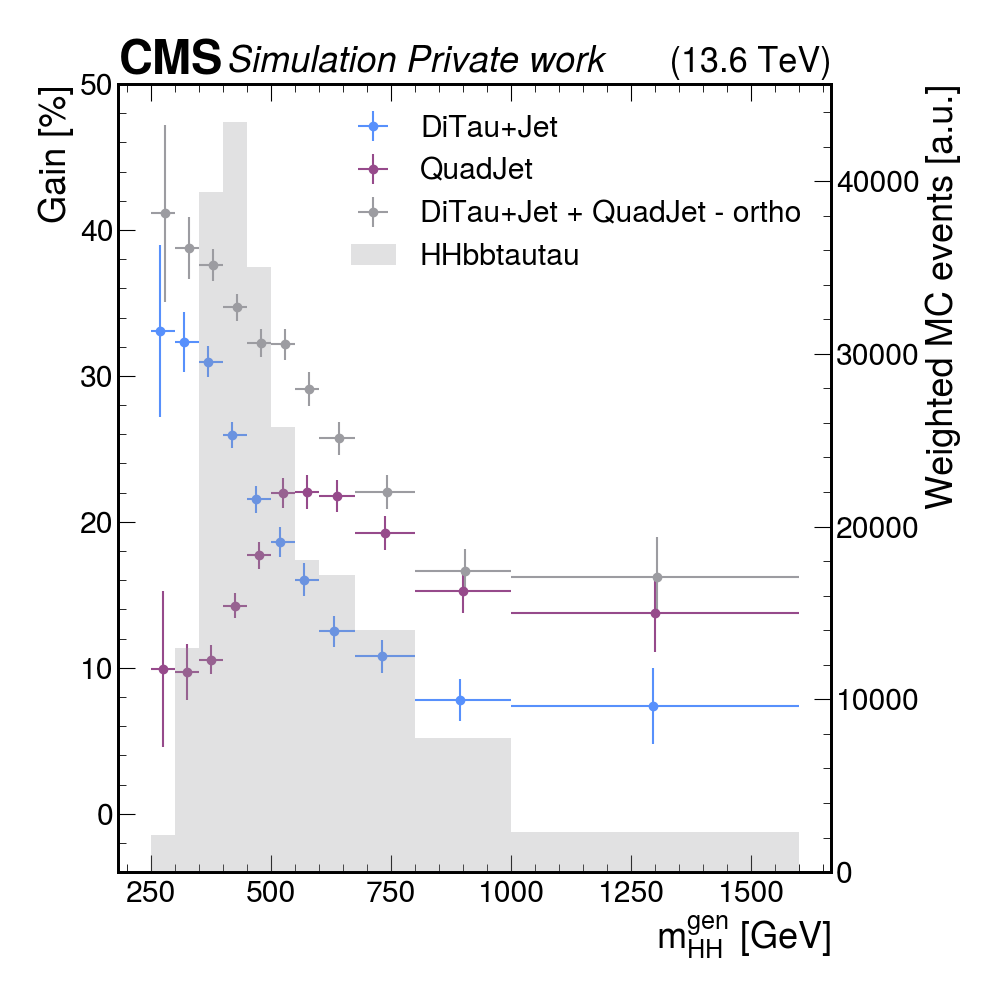
\includegraphics[width=\linewidth]{figures/chapter_V/trigger_gain_kl1.png}
        \caption{$\kappa_{\lambda} = 1$}
        \label{fig:trigger_gain_kl1}
    \end{subfigure}
    \hfill
    \begin{subfigure}[b]{0.49\linewidth}
        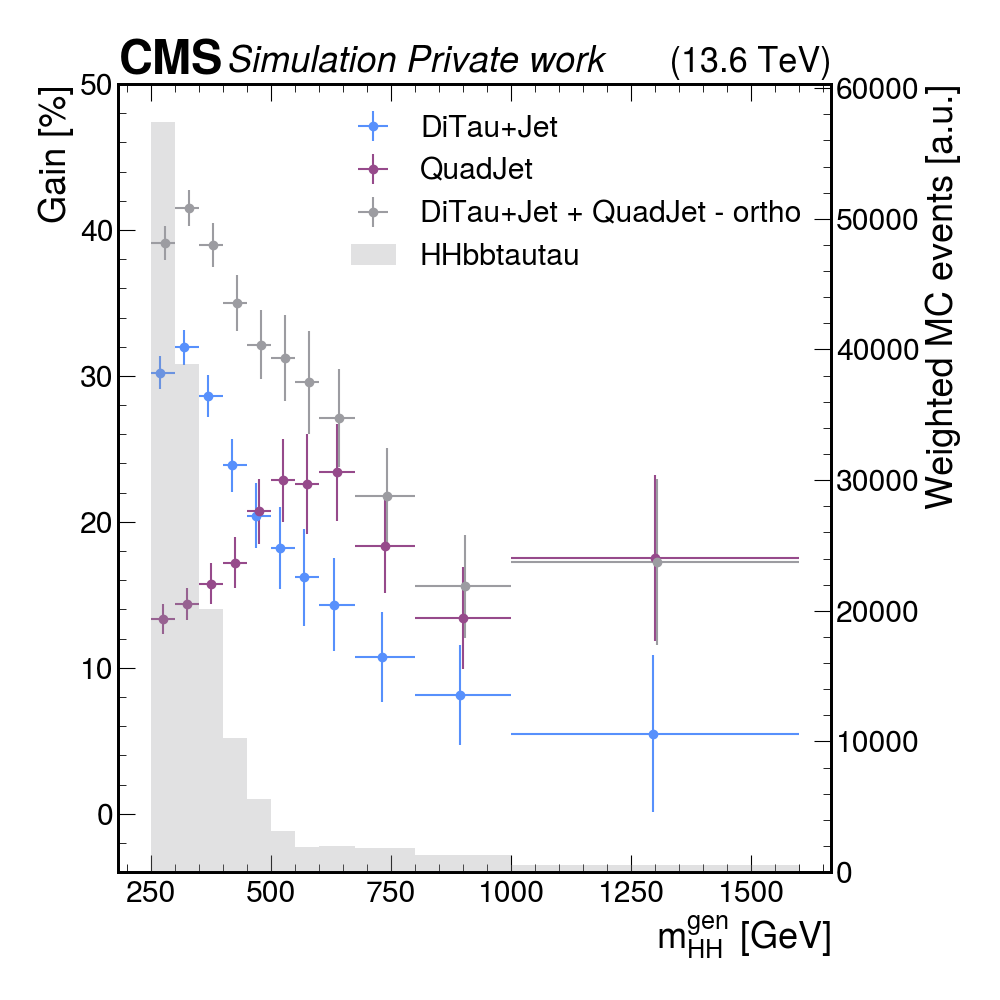
\includegraphics[width=\linewidth]{figures/chapter_V/trigger_gain_kl5.png}
        \caption{$\kappa_{\lambda} = 5$}
        \label{fig:trigger_gain_kl5}
    \end{subfigure}
    \caption[Signal efficiency gain from the new Run 3 trigger paths]{%
        Gain in the selection efficiency of the ggF signal of the DiTau$+$Jet path (blue), the QuadJet parking
        path (purple), and their orthogonalized combination (gray), relative to the DiTau path
        alone, as a function of the generator-level $HH$ invariant mass, in the
        $\tau_{h}\tau_{h}$ final state. The $m_{HH}$ distribution of the ggF signal, in arbitrary units, is
        superimposed in light gray.}
    \label{fig:trigger_gain}
\end{figure}

Paths dedicated to the VBF topology, mostly recorded through the parking stream from 2023 onwards, extend the single path of this kind used in Run 2, and select the two VBF jets either alone, in the so-called \textit{inclusive} path, or together with a muon, an electron, or one or two $\tau_h$. They are chosen separately for each final state according to their gain in signal efficiency and their overlap with the paths already in use, which results in the VBF+$\mu$ path in $\tau_\mu\tau_h$, the inclusive and VBF+$e$ paths in $\tau_e\tau_h$, and the inclusive path together with those requiring one or two $\tau_h$ in $\tau_h\tau_h$. In all channels, the gain is largest at low invariant mass, and it is considerably larger in $\tau_h\tau_h$ than in the semileptonic channels, since the single-lepton and cross-lepton paths already cover the latter effectively, whereas in the fully hadronic case the baseline requires two $\tau_h$ above $35$ GeV ($30$ GeV in 2024), leaving much greater room for improvement.\medskip



%Los caminos VBF se combinan siempre entre sí mediante disyunción lógica, si bien en $\tau_h\tau_h$ el conjunto se considera únicamente para los sucesos que no satisfacen las selecciones de los caminos de doble $\tau_h$ y del camino hadrónico de parking

Finally, Run 3 incorporates two paths that give access to the boosted $\tau_h\tau_h$ channel, where the decay products of the two $\tau$ leptons are too collimated for the double $\tau_h$ path. The first requires large $p_T^\text{miss}$, computed without the muon contribution, which in this regime is larger than in the resolved one, where the two $\tau$ leptons are emitted in nearly opposite directions. The second requires a large-radius jet with a minimum soft-drop mass\footnote{The soft-drop mass is the mass of the jet after removing its soft, wide-angle radiation, which makes it a more faithful estimator of the mass of the particle that originated it~\cite{Larkoski:2014wba}.}, tagged online by a discriminator trained to distinguish $H \to \tau\tau$ from multijet production. The two paths are complementary in simulated signal events, since the efficiency of the first reaches its plateau only for an offline $p_T^\text{miss}$ of about $200$ GeV, while the second is most efficient precisely at lower $p_T^\text{miss}$. For simplicity, they are applied in mutually exclusive regions separated by this threshold, with only a small loss of efficiency with respect to their logical OR.





% For two jets, the leading and subleading values
%   are quoted in that order. The 2024 changes follow the migration of the online $\tau_{h}$
%   identification from \textsc{DeepTau} to \textsc{ParticleNet}, which allowed the
%   thresholds to be lowered and the acceptance extended in $|\eta|$; in the VBF parking
%   paths the jet and $m_{jj}$ requirements were instead tightened, and the $\Delta\eta_{jj}$
%   requirement was dropped altogether. The working point of the online $H\to\tau\tau$ tagger
%   was loosened from $0.30$ to $0.03$ already during 2023, following a retraining of the
%   algorithm. The QuadJet and VBF paths other than VBF$+$DiTau are recorded through the
%   parking streams. 

% The quoted  thresholds correspond to the 2022 and 2023 data taking; for two jets, the leading and  subleading values are given in that order. All thresholds were re-optimized for 2024,  when the online $\tau_{h}$ identification moved from \textsc{DeepTau} to  \textsc{ParticleNet}, allowing the DiTau threshold to be lowered to $30$ GeV and the  acceptance to be extended to $|\eta| < 2.3$. The VBF parking paths were redefined more  substantially for that year, with higher jet and $m_{jj}$ thresholds and no  $\Delta\eta_{jj}$ requirement. The working point of the online $H\to\tau\tau$ tagger was  loosened from $0.30$ to $0.03$ during 2023 following a retraining of the algorithm. The  QuadJet and VBF paths other than VBF$+$DiTau are recorded through the parking streams.  Within each final state the logical OR of all applicable paths is used, with the exception  of the QuadJet path, which is applied in an orthogonal region of phase space.



% Thresholds correspond to the 2022 and 2023 data taking; for two jets, the leading and subleading values are quoted as $p_{T} > x\,(y)$. All thresholds were re-optimized for 2024, when the online $\tau_{h}$ identification moved from \textsc{DeepTau} to \textsc{ParticleNet}, allowing the DiTau threshold to be lowered to $30$ GeV and the acceptance to be extended to $|\eta| < 2.3$. The working point of the online $H\to\tau\tau$ tagger was likewise loosened from $0.30$ to $0.03$ during 2023 following a retraining of the algorithm. The QuadJet and VBF paths other than VBF$+$DiTau are recorded through the parking streams. The VBF inclusive path is used in the $e\tau_{h}$ and $\tau_{h}\tau_{h}$ final states only. Within each final state the logical OR of all applicable paths is used, with the exception of the QuadJet path, which is applied in an orthogonal region of phase space.


\section{Physics object preselection}
\label{sec:bbtt_objects}
%
The objects of the $bb\tau\tau$ final state — muons, electrons, hadronic $\tau$ leptons, jets, and the missing transverse momentum — are reconstructed from the Particle Flow candidates as described in Section \ref{sec:POR}. This section therefore only lists the identification criteria and the kinematic regions that define each object at the analysis level. Their $p_T$ thresholds are not set here but inherited from the trigger that selected each event, since the objects of the final state must be matched within $\Delta R < 0.5$ to those that fired it and exceed a threshold
%
\begin{equation}
    p_{T}^{\text{offline}} \geq p_{T}^{\text{online}} + \delta,
    \label{eq:trigger_matching}
\end{equation}
%
where $p_{T}^{\text{online}}$ is the online threshold listed in Table \ref{tab:triggers} and $\delta$ is a margin that places the selection on the plateau of the efficiency curve rather than on its turn-on. This margin is determined by the resolution with which each type of object is reconstructed online versus offline, and it is set at $1$ GeV for electrons, $2$ GeV for muons, and $5$ GeV for hadronic $\tau$ leptons\footnote{The thresholds on the hadronic legs are those applied online, except for the VBF+DiTau path, whose two jets must have $p_{T} > 140$ $(160)$ and $60$ $(70)$ GeV in 2022--2023 (2024), and for the $p_T^\text{miss}$ path, whose slower turn-on requires $p_T^\text{miss} > 200$ GeV.}. The preselections described below are therefore deliberately loose in $p_T$.

\subsection{Muons and electrons}
%
Muons are selected within the acceptance of the muon system, $|\eta| < 2.4$, with the Tight identification working point and a relative isolation below $0.15$ in a cone of $\Delta R = 0.4$. Electrons are restricted to the tracker coverage, $|\eta| < 2.5$, and identified with a multivariate discriminant that combines identification and isolation, at the working point with $80\%$ efficiency; in 2022postEE, those in the region of the endcap affected by the incident described in Section \ref{sec:bbtt_samples} are discarded. Both must be compatible with the primary vertex, with transverse and longitudinal impact parameters below $0.045$ and $0.2$ cm. Events with an additional muon or electron passing looser criteria are rejected, which suppresses the Drell--Yan and dileptonic $t\bar{t}$ contributions.


\subsection{Hadronic tau leptons}
%
%Hadronic $\tau$ leptons are reconstructed using the \textit{hadrons-plus-strips} algorithm and identified using \textsc{DeepTau} 2018 v2.5, as described in Section \ref{sec:DeepTau2.5}. Candidates with $p_T > 20$ $(25)$ GeV and $|\eta| < 2.5$ are accepted, provided they are compatible with the primary vertex via $|d_z| < 0.2$ cm, and reconstructed in one of the decay modes with one or three charged hadrons, with or without associated neutral pions. Against electrons, the VVLoose working point is required in all channels; against muons, the Tight working point is used in the semileptonic channels and the VLoose one in $\tau_h\tau_h$, where contamination from light leptons is negligible. For jets, however, preselection is maintained at the loosest available working point, \textit{VVVLoose}; the \textit{Medium} point, which defines the signal region, is applied later, so that the band between the two remains available for constructing the control regions used to estimate the misidentified jet background. In the boosted channel, where the two $\tau$ particles are so collimated that their decay products fall within the same jet, the candidates come from the dedicated reconstruction described in Chapter \ref{ch:Tau} and are identified using the version of \textsc{DeepTau} trained specifically for this regime.

Hadronic $\tau$ leptons are reconstructed with the hadrons-plus-strips algorithm and identified using \textsc{DeepTau} 2018 v2.5 (Section \ref{sec:DeepTau2.5}). Candidates with $p_T > 20$ GeV, $|\eta| < 2.5$, and $|d_z| < 0.2$ cm are accepted if reconstructed in a decay mode with one or three charged hadrons, with or without neutral pions. In the resolved channels, the discriminant against electrons is required at the VVLoose WP; against muons, the Tight WP is used in the semileptonic channels and the VLoose one in $\tau_h\tau_h$, where the contamination from light leptons is negligible. Against jets, only the loosest WP, VVVLoose, is required at this stage. The Medium WP, which defines the signal region, is applied later, so that the candidates between the two remain available for estimating the misidentified jet background. In the boosted $\tau_h\tau_h$ channel, the candidates come from the dedicated reconstruction described in Section \ref{subsec:Taus} and are identified with the version of \textsc{DeepTau} trained for this regime, with the same preselection and a threshold that rises to $25$ GeV in 2024.


\subsection{Jets and heavy-flavor identification}
%
Jets are clustered from the Particle Flow candidates with the anti-$k_T$ algorithm, with $R = 0.4$, and with $R = 0.8$ for boosted topologies. Those overlapping with the selected $\tau$ candidates are removed, as are those with $p_T < 50$ GeV in the transition region $2.5 < |\eta| < 3.0$, where the resolution degrades. The $b$ jet candidates are sought among the jets with $p_T > 20$ GeV and $|\eta| < 2.5$, and the VBF jet candidates up to $|\eta| < 4.7$, the full coverage of the forward calorimeter. Central jets are $b$ tagged with \textsc{ParticleNet} in 2022 and 2023 and with \textsc{UParT} in 2024, the algorithm recommended for each campaign, with centrally provided working points and corrections. Large-radius jets must have $p_T > 250$ GeV, $|\eta| < 2.5$, and a soft-drop mass above $30$ GeV, and are ranked by a \textsc{ParticleNet} discriminant that separates $H\to b\bar{b}$ decays contained in a single jet from multijet production. The jets that form each candidate are chosen by the algorithms of Chapter \ref{ch:taggers}, as described in the next section.


% The jets are reconstructed by grouping Particle Flow candidates using the anti-$k_T$ algorithm, with a distance parameter of $R = 0.4$ for ordinary jets and $R = 0.8$ for large-radius jets intended for boosted topologies. Of these, those that overlap with the already selected $\tau$ candidates are discarded to avoid double-counting the same energy deposits, as are low-momentum jets reconstructed in the transition region $2.5 < |\eta| < 3.0$, where the resolution degrades significantly. The $b$ jet candidates are sought among jets with $p_T > 20$ GeV and $|\eta| < 2.5$, while vector boson fusion jet candidates are accepted up to $|\eta| < 4.7$, taking advantage of the complete coverage of the forward hadronic calorimeter. Among the central jets, those originating from the hadronization of a $b$ quark are identified with \textsc{ParticleNet} in the 2022 and 2023 periods and \textsc{UParT} in 2024, in each case the one recommended for the corresponding campaign, with the working points and their associated corrections taken from the centralized calibrations provided by the collaboration. Large-radius jets, on the other hand, are required to have $p_T > 250$ GeV, $|\eta| < 2.5$, and a soft-drop mass greater than $30$ GeV, and are ranked by a dedicated \textsc{ParticleNet} discriminant trained to separate a $H \to b\bar{b}$ decay reconstructed within a single jet from multijet production. The decision of which jets to include in the reconstruction of each candidate is made using the algorithms developed in Chapter \ref{ch:taggers}, as described in the following section.

\subsection{Missing transverse momentum}
%
The missing transverse momentum is not preselected, but it enters the reconstruction of the $\tau\tau$ mass, together with its covariance matrix, and the definition of several control and sideband regions. The version computed with the PUPPI weights (Section \ref{subsec:MET}) is used, owing to its reduced sensitivity to pile-up, with the corrections to the energy of the jets and $\tau_h$ candidates propagated to it. The only exception is the threshold that separates the two triggers of the boosted $\tau_h\tau_h$ channel, which is applied to the version computed from all the Particle Flow candidates. In addition, events in which a large and unphysical $p_T^\text{miss}$ can arise from detector noise, beam halo, poorly reconstructed vertices, or misreconstructed muons are rejected with the filters recommended centrally by the collaboration.




% \begin{table}[t]
% \centering
% \small
% \begin{tabular}{l p{7.2cm}}
% \toprule
% \textbf{Variable} & \textbf{Requirement} \\
% \midrule
% \midrule
% \multicolumn{2}{l}{\textit{Muons}} \\
% \midrule
% \quad $p_{T}$ & $> 6$ GeV; the effective threshold is set by the trigger matching, Eq.\ \ref{eq:trigger_matching} \\
% \quad $|\eta|$ & $< 2.4$ \\
% \quad Identification & Tight working point \\
% \quad Isolation & $I_{\text{rel}} < 0.15$, within a cone of $\Delta R = 0.4$ \\
% \quad Impact parameters & $|d_{xy}| < 0.045$ cm, $|d_{z}| < 0.2$ cm \\
% \addlinespace
% \multicolumn{2}{l}{\textit{Electrons}} \\
% \midrule
% \quad $p_{T}$ & $> 12$ GeV; the effective threshold is set by the trigger matching \\
% \quad $|\eta|$ & $< 2.5$ \\
% \quad Identification & Isolation-based multivariate discriminant, working point with $80\%$ signal efficiency \\
% \quad Impact parameters & $|d_{xy}| < 0.045$ cm, $|d_{z}| < 0.2$ cm \\
% \quad Region veto & Endcap region affected by the power loss, 2022postEE only \\
% \addlinespace
% \multicolumn{2}{l}{\textit{Third-lepton veto}} \\
% \midrule
% \quad Additional muons & $p_{T} > 6$ GeV, $|\eta| < 2.4$, medium or tight identification, $I_{\text{rel}} < 0.30$ \\
% \quad Additional electrons & $p_{T} > 10$ GeV, $|\eta| < 2.5$, working point with $90\%$ signal efficiency \\
% \addlinespace
% \multicolumn{2}{l}{\textit{Hadronic $\tau$ leptons, resolved channels}} \\
% \midrule
% \quad $p_{T}$ & $> 20$ GeV; the effective threshold is set by the trigger matching \\
% \quad $|\eta|$ & $< 2.5$ \\
% \quad Impact parameter & $|d_{z}| < 0.2$ cm \\
% \quad Decay mode & One or three charged hadrons, with or without associated neutral pions \\
% \quad \textsc{DeepTau} against jets & $\geq$ VVVLoose at preselection; Medium in the signal region \\
% \quad \textsc{DeepTau} against $e$ & $\geq$ VVLoose \\
% \quad \textsc{DeepTau} against $\mu$ & $\geq$ Tight in $\tau_\mu\tau_h$ and $\tau_e\tau_h$; $\geq$ VLoose in $\tau_h\tau_h$ \\
% \addlinespace
% \multicolumn{2}{l}{\textit{Hadronic $\tau$ leptons, boosted channel}} \\
% \midrule
% \quad $p_{T}$ & $> 20$ GeV \\
% \quad $|\eta|$ & $< 2.5$ \\
% \quad Decay mode & One or three charged hadrons, with or without associated neutral pions \\
% \quad \textsc{BoostedDeepTau} & Discriminants against jets, $e$ and $\mu$ above $0.72$, $0.1$ and $0.003$ \\
% \addlinespace
% \multicolumn{2}{l}{\textit{Jets of radius $R = 0.4$}} \\
% \midrule
% \quad Identification & Tight working point \\
% \quad Cleaning & $\Delta R > 0.5$ from both $\tau$ candidates \\
% \quad Transition region & Jets with $p_{T} < 50$ GeV in $2.5 < |\eta| < 3.0$ are discarded \\
% \quad $b$ jet candidates & $p_{T} > 20$ GeV, $|\eta| < 2.5$ \\
% \quad VBF jet candidates & $p_{T} > 20$ GeV, $|\eta| < 4.7$ \\
% \addlinespace
% \multicolumn{2}{l}{\textit{Jets of radius $R = 0.8$}} \\
% \midrule
% \quad $p_{T}$ & $> 250$ GeV \\
% \quad $|\eta|$ & $< 2.5$ \\
% \quad Soft-drop mass & $> 30$ GeV \\
% \quad Cleaning & $\Delta R > 0.8$ from the $\tau$ candidates \\
% \addlinespace
% \multicolumn{2}{l}{\textit{$\tau\tau$ pair}} \\
% \midrule
% \quad Charge & The two candidates of opposite charge \\
% \quad Separation & $\Delta R > 0.5$ between them \\
% \bottomrule
% \end{tabular}
% \caption[Physics object selection criteria]{%
%   Identification and acceptance criteria defining the physics objects used in the analysis.
%   The transverse momentum thresholds quoted are preselection floors: the threshold that
%   actually applies to a given event is the one imposed by the matching to the trigger path
%   that selected it.}
% \label{tab:object_selection}
% \end{table}


\section{Event selection and categorization}
\label{sec:bbtt_flow}
%
The criteria defining each of the analysis objects separately have been established. However, the analysis rests on the combinations they form among themselves so that the event is assembled candidate by candidate, following a specific order. First, the pair $\tau\tau$ is reconstructed, since it determines the channel to which the event is assigned. Next, the candidate $H\to b\bar{b}$ is constructed, removing from the jet collection those overlapping with the $\tau$ candidates once they have been selected. Finally, the jets remaining after the two Higgs boson candidates have been formed are examined for the topology characteristic of vector boson fusion.

Once the candidates have been identified, the analysis proceeds to the definition of the signal regions. Events are first distributed among mutually exclusive categories, defined by the topology in which the event was reconstructed and by the final state of the $\tau\tau$ pair. Within the resolved categories, a requirement on the plane defined by the two reconstructed masses then removes the region where no signal is expected. It is therefore essential to address how the mass of each candidate is reconstructed, as will be done in each of the corresponding sections. These categories represent the regions from which the signal is ultimately extracted and, therefore, the way they are defined has a direct impact on the final results of the analysis. The whole sequence is summarized in Figure \ref{fig:category_flow}, whose numbered steps the following sections walk through in the order in which they are applied.
%
\begin{figure}[tbp]
\centering
\definecolor{recBg}{HTML}{F1F6FC}\definecolor{recLn}{HTML}{9BBDE3}
\definecolor{catBg}{HTML}{ECF7F5}\definecolor{catLn}{HTML}{72B9B1}
\definecolor{outBg}{HTML}{F2F2F4}\definecolor{outLn}{HTML}{AEAEB8}
\newcommand{\ffont}{\fontfamily{Nunito-TLF}\selectfont}
\begin{tikzpicture}[
    x=1mm, y=1mm, font=\ffont\footnotesize,
    box/.style   = {draw=#1, line width=0.6pt, rounded corners=3pt, fill=white,
                    align=center, inner sep=2pt},
    res/.style   = {draw=outLn, line width=0.6pt, rounded corners=3pt, fill=outBg,
                    align=center, inner sep=2pt, minimum height=6mm, minimum width=26mm,
                    font=\ffont\footnotesize\bfseries},
    num/.style   = {circle, fill=#1, text=white, font=\ffont\tiny\bfseries,
                    inner sep=0pt, minimum size=3.6mm},
    ar/.style    = {-{Latex[length=1.8mm]}, draw=catLn!85!black, line width=0.6pt},
    lbl/.style   = {font=\ffont\scriptsize, text=catLn!85!black, inner sep=1.2pt},
    title/.style = {font=\ffont\footnotesize\bfseries\boldmath, text=#1!75!black, anchor=north, inner sep=0pt},
    head/.style  = {font=\ffont\footnotesize\bfseries\boldmath, inner sep=0pt},
    sub/.style   = {font=\ffont\scriptsize, inner sep=0pt},
    block/.style = {draw=#1Ln, fill=#1Bg, line width=0.6pt, rounded corners=5pt,
                    inner xsep=4mm, inner ysep=3.5mm},
    chip/.style  = {draw=outLn, line width=0.5pt, rounded corners=2pt, fill=outBg,
                    font=\ffont\footnotesize\bfseries\boldmath, inner sep=1pt,
                    minimum height=5.5mm, minimum width=16mm}
  ]
  % ================= candidate reconstruction
  % H->bb and VBF stacked on the right, H->tautau spanning both on the left
  \node[box=recLn, minimum width=52mm, minimum height=10mm] (bb)  at (96,0)   {};
  \node[box=recLn, minimum width=52mm, minimum height=10mm] (vbf) at (96,-13) {};
  \node[box=recLn, minimum width=52mm, minimum height=23mm] (tt)  at (30,-6.5) {};
  \node[head] at ([yshift=-3.3mm]bb.north)  {$H\to b\bar{b}$ candidate};
  \node[sub]  at ([yshift=3.0mm]bb.south)   {resolved \quad boosted};
  \node[head] at ([yshift=-3.3mm]vbf.north) {VBF jet pair};
  \node[sub]  at ([yshift=3.0mm]vbf.south)  {among the remaining jets};
  \node[head] at ([yshift=-3.3mm]tt.north)  {$H\to\tau\tau$ candidate};
  \foreach \dx/\dy/\t in {-9/-10/{$\tau_\mu\tau_h$}, 9/-10/{$\tau_e\tau_h$},
                          -9/-17/{$\tau_h\tau_h$}, 9/-17/{$b\tau_h\tau_h$}}
    \node[chip] at ([xshift=\dx mm, yshift=\dy mm]tt.north) {\t};
  \coordinate (rtop) at ([yshift=4.5mm]tt.north);
  % ================= categorization
  \node[box=catLn, minimum width=62mm, minimum height=6.5mm] (d1) at (36,-36) {\textbf{Boosted {\boldmath$H\to b\bar{b}$} candidate?}};
  \node[box=catLn, minimum width=62mm, minimum height=6.5mm] (d2) at (36,-47) {\textbf{VBF topology?}};
  \node[box=catLn, minimum width=62mm, minimum height=6.5mm] (d3) at (36,-58) {\textbf{How many {\boldmath$b$}-tagged jets?}};
  \node[res] (cb) at (109,-36) {boosted};
  \node[res] (cv) at (109,-47) {VBF};
  \node[res] (c2) at (109,-54) {res2b};
  \node[res] (c1) at (109,-62) {res1b};
  \coordinate (ctop) at ([yshift=4.5mm]d1.north);
  % ================= step numbers, inside each box at the top right
  \foreach \n/\k/\c in {tt/1/recLn, bb/2/recLn, vbf/3/recLn, d1/4/catLn, d2/5/catLn, d3/6/catLn}
    \node[num=\c, anchor=north east] at ([xshift=-3.5pt,yshift=-3.5pt]\n.north east) {\k};
  % ================= arrows
  \draw[ar] (d1) -- (d2) node[lbl, midway, right, xshift=1mm] {no};
  \draw[ar] (d2) -- (d3) node[lbl, midway, right, xshift=1mm] {no};
  \draw[ar] (d1) -- (cb) node[lbl, midway, above] {yes};
  \draw[ar] (d2) -- (cv) node[lbl, midway, above] {yes};
  \draw[ar] (d3.east) -- ++(8,0) |- (c2.west) node[lbl, pos=0.78, above] {two};
  \draw[ar] (d3.east) -- ++(8,0) |- (c1.west) node[lbl, pos=0.78, below] {one};
  % ================= blocks, drawn behind; the top coordinate leaves room for the title
  \begin{pgfonlayer}{background}
    \node[block=rec, fit=(rtop)(tt)(bb)(vbf)(cb.east |- tt)] (recblock) {};
    \node[block=cat, fit=(ctop)(d1)(d3)(cb)(c1)(tt.west |- d1)] (catblock) {};
  \end{pgfonlayer}
  \node[title=recLn] at ([yshift=-2.5mm]recblock.north) {CANDIDATE RECONSTRUCTION};
  \node[title=catLn] at ([yshift=-2.5mm]catblock.north) {CATEGORIZATION};
\end{tikzpicture}
\caption[Category assignment scheme]{Sequence followed to reconstruct the candidates of each event and assign it to a category, with the steps numbered in the order in which they are applied.}
\label{fig:category_flow}
\end{figure}



\subsection{\texorpdfstring{$H\to\tau\tau$}{H->tautau}: the channel-defining pair}
% FINAL STATES ASSIGNMENT AND SELECTION
%
After the preselection described in Section \ref{sec:bbtt_objects}, the channel of each event is determined by its light lepton content. Events with one muon and no electron are assigned to the $\tau_\mu\tau_h$ channel and those with one electron and no muon to the $\tau_e\tau_h$ channel, provided they contain at least one $\tau_h$ candidate, while events with no light leptons and at least two $\tau_h$ candidates are assigned to the $\tau_h\tau_h$ channel. Events with two light leptons, $\mu\mu$, $ee$, or $e\mu$, are kept separately and reserved as control regions, since there the signal is negligible compared with Drell--Yan production in the first two and with dileptonic $t\bar{t}$ decays in the third. All other events are discarded.

Since the $\tau_h$ candidates are preselected with the loosest working point against jets -- to allow the estimation of the misidentified jet background described in Section \ref{sec:bbtt_ff} -- a single event often admits several pairs compatible with its channel. All of them are ranked, and the first one is retained. The ranking compares first the isolation of the leading leg, which for a $\tau_h$ is its \textsc{DeepTau} score against jets, then its $p_T$, and then the same two quantities for the second leg. In the semileptonic channels the light lepton is always the leading leg, while in $\tau_h\tau_h$ both orderings are considered. The pair retained is therefore the one least likely to contain a misidentified jet.

The boosted $\tau_h\tau_h$ channel is considered only for events without light leptons in which no resolved pair is found, so that the resolved channel always takes precedence. The two candidates from the dedicated reconstruction are paired if their angular separation lies between $0.05$ and $0.8$, close enough to be contained in a large-radius jet but not so close as to be two reconstructions of the same object. The pair is then associated with the large-radius jet that contains it, the one with the highest $p_T$ if there are several, and is retained only if a \textsc{ParticleNet} discriminant evaluated on that jet, which quantifies its compatibility with an $H\to\tau\tau$ decay against multijet production, exceeds $0.1$\textcolor{red}{, below which the efficiency of the corresponding trigger path is not reliably described by the simulation}.\medskip

\subsubsection{\texorpdfstring{$H\to\tau\tau$}{H->tautau} mass reconstruction}
%
Every $\tau$ decay contains at least one neutrino that escapes detection, so that the invariant mass of the visible decay products is shifted well below $125$ GeV and has a large width. In Run 2, the mass was instead estimated with the SVfit algorithm~\cite{fastmtt}, a likelihood method that evaluates the compatibility of each mass hypothesis with the measured momenta of the visible products and with $p_T^\text{miss}$, of which \textsc{FastMTT}~\cite{Kalinowski:2025vci} is a faster, simplified version. In Run 3, this method is replaced by a neural network that regresses the momenta of the neutrinos, so that the mass follows from the sum of the reconstructed four-momenta. The network receives categorical variables describing the event -- such as the channel and the decay mode and charge of each $\tau$ -- together with the four-momenta of the $\tau$ and $b$ jet candidates and of the systems they form, $p_T^\text{miss}$ with its covariance matrix, and the jet tagging scores. It is trained separately for each period on signal and on Drell--Yan, $t\bar{t}$, and $t\bar{t}H$ samples, and the boosted events, too few for training, are evaluated as $\tau_h\tau_h$.

Figure \ref{fig:htautau_mass} compares the three estimates in the $\tau_\mu\tau_h$ channel. The visible mass places the signal around $70$ GeV, completely overlapping with the Drell--Yan peak. \textsc{FastMTT} recovers the scale but leaves a width comparable to the distance between the two peaks, while the regression concentrates the signal in a narrow peak around $122$ GeV, clearly separated from Drell--Yan. The resolution improves by about $80\%$ ($75\%$) for the ggF (VBF) signal with respect to \textsc{FastMTT}, and the background rejection by $50$ ($39$) to $55\%$ ($48\%$) depending on the channel. In the purely leptonic control channels, which do not enter the signal extraction, \textsc{FastMTT} is still used.
%The resolution is quantified as σ/μ of a Gaussian fit to the core of the signal peak; the background rejection is evaluated in the narrowest mass window containing 68% of the signal, so that all methods are compared at the same signal efficiency.
%RESOLUCION:Para cada método se ajusta una gaussiana solo a la parte central del pico de la señal, sin las colas:
% Se empieza con μ en el bin más alto y σ igual al RMS del histograma.
% Se ajusta una gaussiana en el intervalo [μ − 1.5σ, μ + 1.5σ].
% Con los μ y σ nuevos se repite el ajuste, hasta que dejan de cambiar.
% El resultado es la posición del pico, μ (los valores X e Y de tu frase), y su anchura, σ. La resolución relativa es σ/μ, y la mejora es cuánto se reduce σ/μ al pasar de FastMTT a la regresión:
% mejora = 1 − (σ/μ)<sub>regresión</sub> / (σ/μ)<sub>FastMTT</sub>
%REDUCCION DE FONDOS
% No tendría sentido comparar el fondo en una ventana fija, porque los picos tienen anchuras muy distintas. En su lugar se compara cuánto fondo hay que aceptar para quedarse con la misma fracción de señal:
% Para cada método se busca la ventana de masa más estrecha que contiene el 68 % de la señal. Si el último bin solo se necesita en parte, se toma la fracción necesaria suponiendo el contenido uniforme dentro del bin, para que la eficiencia sea exactamente 0.68 en todos los métodos.
% Se integra el fondo (total, y aparte solo el DY) dentro de esa misma ventana.
% La reducción es:
% reducción = 1 − B<sub>regresión</sub> / B<sub>FastMTT</sub>
% Canal	Pico visible	Pico FastMTT (σ/μ)	Pico regresión (σ/μ)	Mejora en σ/μ	Menos fondo total	Menos DY
% μτ	70 GeV	113 GeV (17 %)	122 GeV (3.2 %)	81 %	55 %	72 %
% eτ	73 GeV	114 GeV (16 %)	122 GeV (3.4 %)	79 %	52 %	61 %
% τhτh	84 GeV	114 GeV (16 %)	121 GeV (2.8 %)	82 %	50 %	62 %
%
\begin{figure}[tbp]
    \centering
    \begin{subfigure}[b]{0.32\linewidth}
        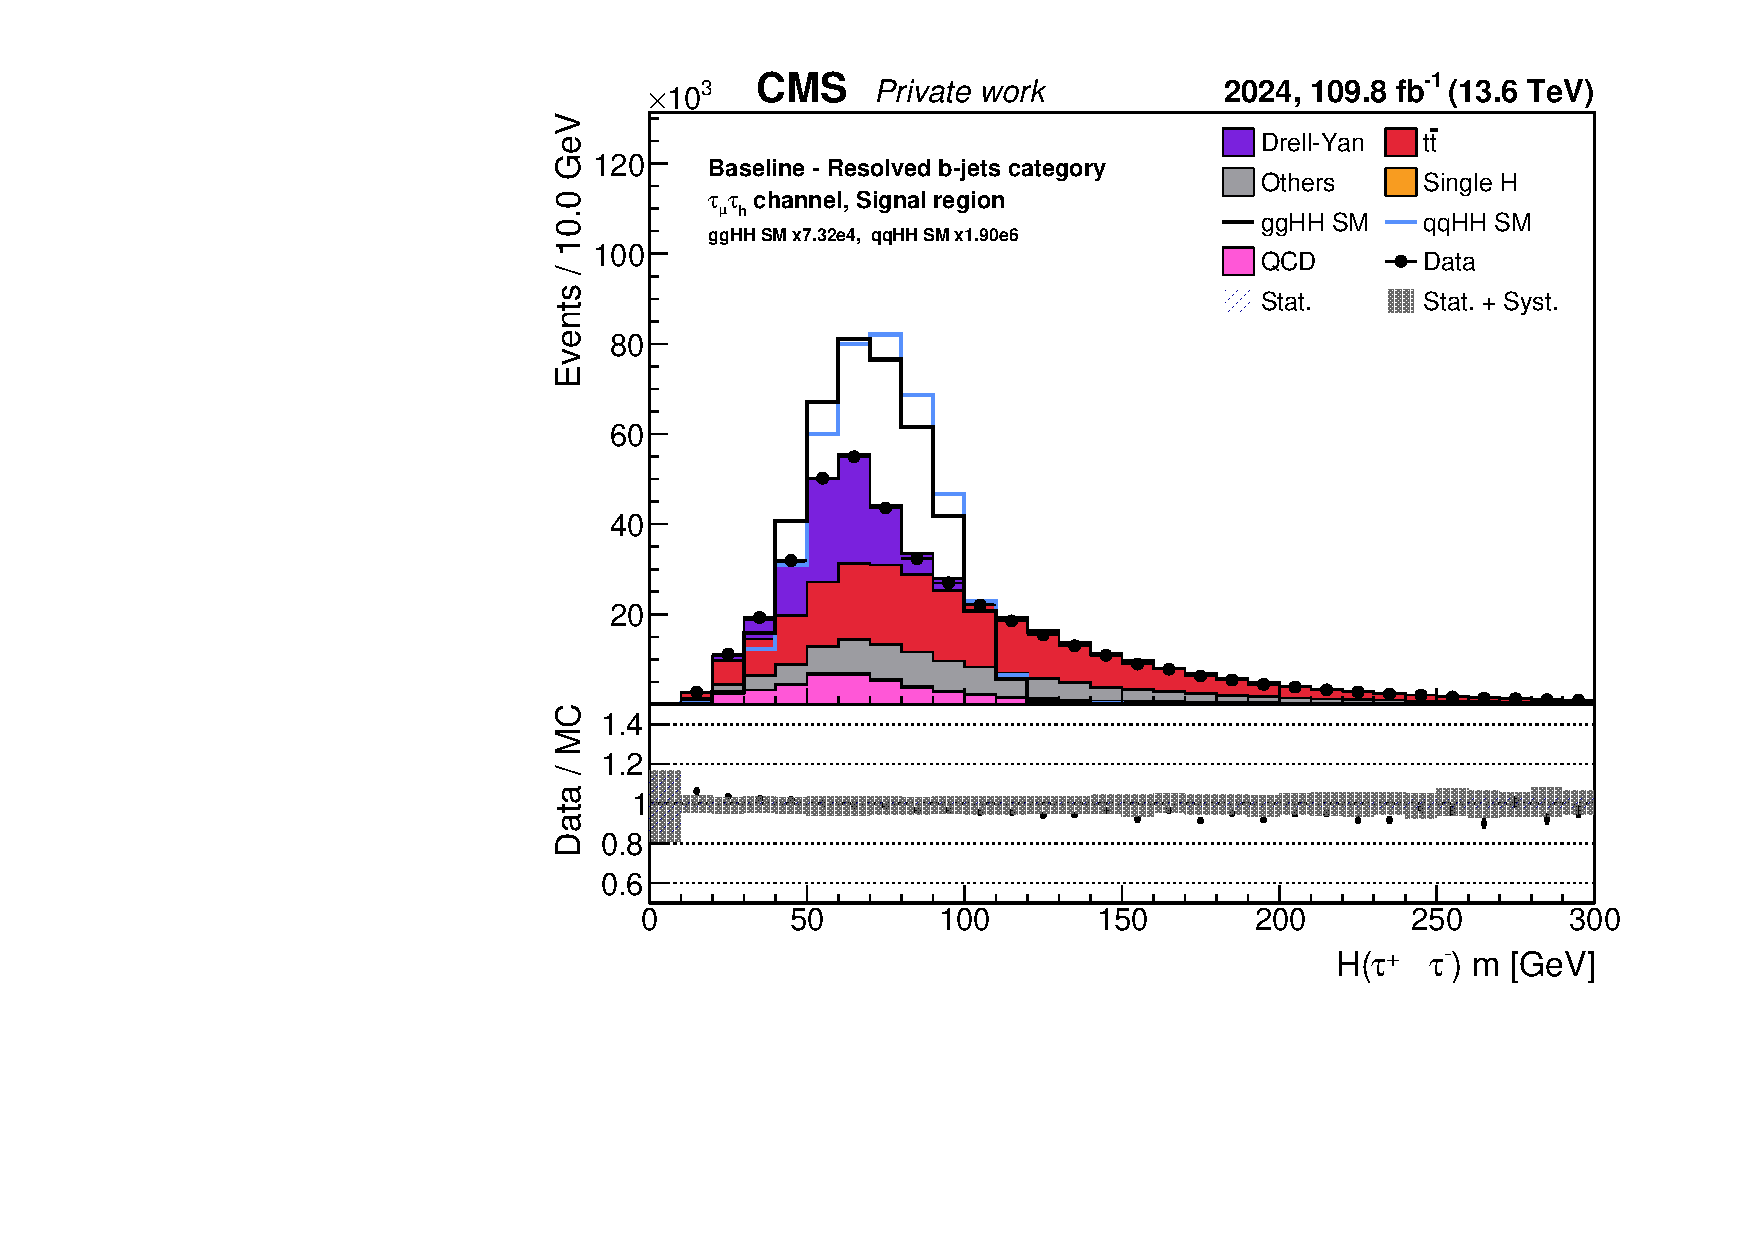
\includegraphics[width=\linewidth, trim=11bp 0bp 40bp 14bp, clip]{figures/chapter_V/Htt_mass__mutau_os_iso__pg_forPlots__qcd__stack__norm_sig.pdf}
        \caption{Visible mass}
        \label{fig:htt_mass_vis}
    \end{subfigure}\hfill
    \begin{subfigure}[b]{0.32\linewidth}
        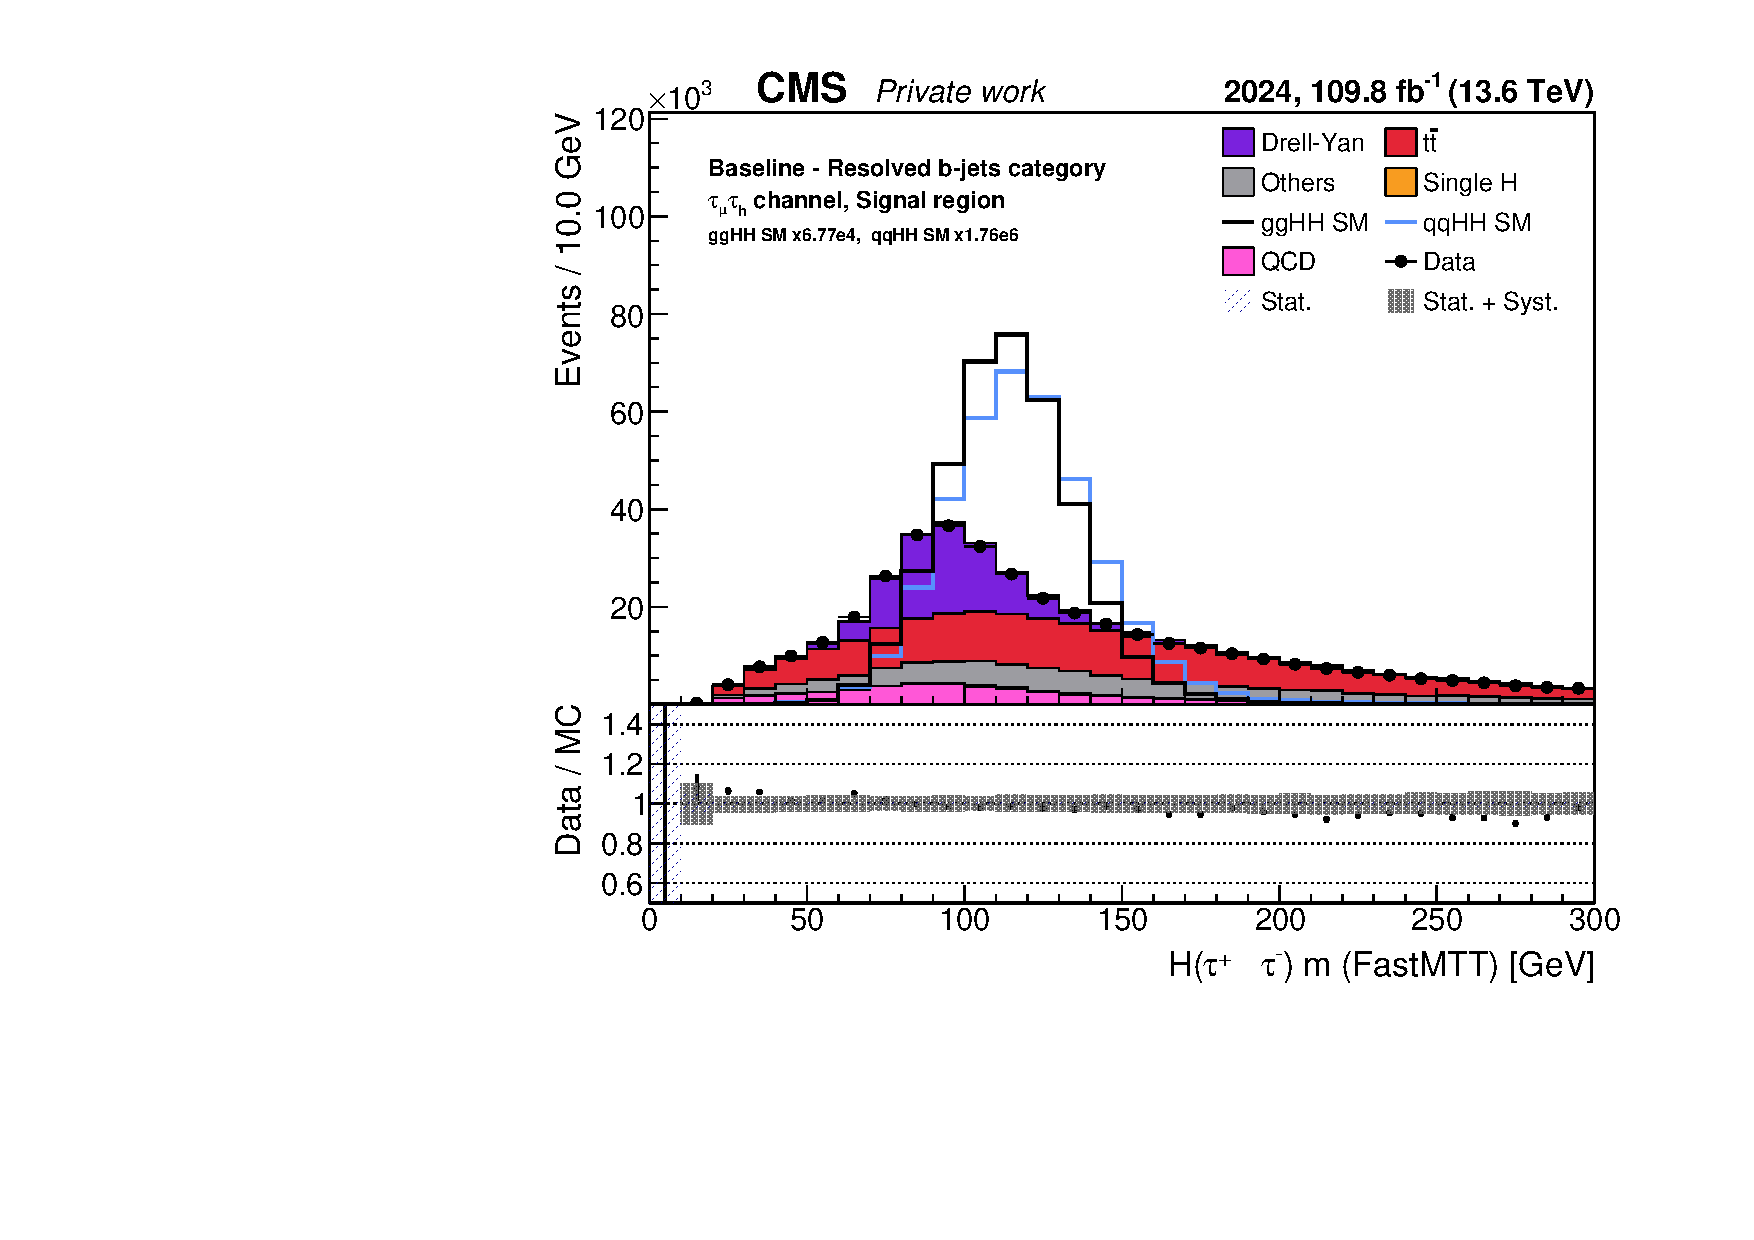
\includegraphics[width=\linewidth, trim=11bp 0bp 40bp 14bp, clip]{figures/chapter_V/Htt_svfit_mass__mutau_os_iso__pg_forPlots__qcd__stack__norm_sig.pdf}
        \caption{\textsc{FastMTT}}
        \label{fig:htt_mass_fastmtt}
    \end{subfigure}\hfill
    \begin{subfigure}[b]{0.32\linewidth}
        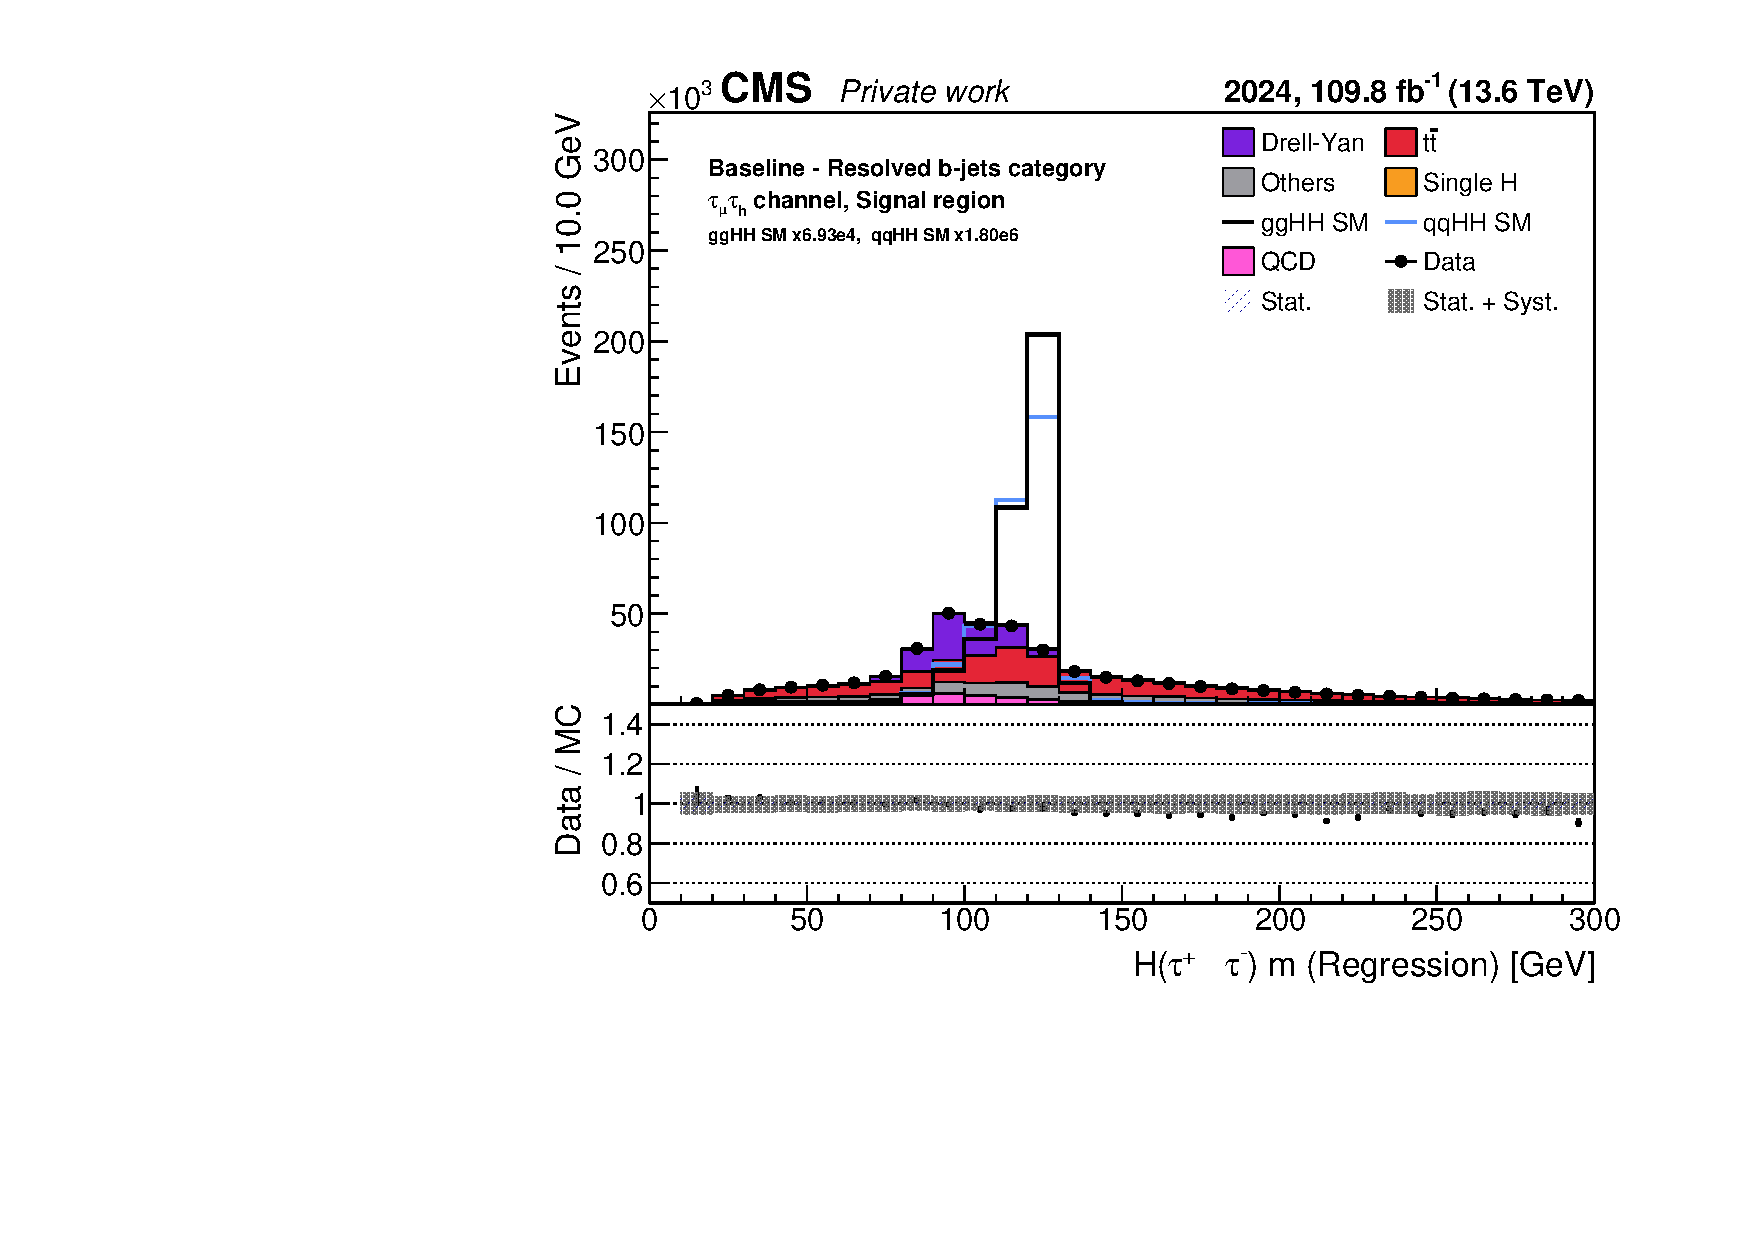
\includegraphics[width=\linewidth, trim=11bp 0bp 40bp 14bp, clip]{figures/chapter_V/Htt_regr_mass__mutau_os_iso__pg_forPlots__qcd__stack__norm_sig.pdf}
        \caption{Regression network}
        \label{fig:htt_mass_regr}
    \end{subfigure}
    \caption[Reconstruction of the $\tau\tau$ system mass]{Mass of the $\tau\tau$ system reconstructed from the visible decay products (a), with \textsc{FastMTT} (b), and with the regression network (c), in the $\tau_\mu\tau_h$ channel and the resolved topology, with no requirement on the reconstructed masses, for the 2024 data. The points show the data and the stacked histograms the background prediction, while the ggF (black) and VBF (blue) signals are scaled to the total background yield. The lower panels show the ratio of the data to the prediction, with the statistical and total uncertainty bands.}
    \label{fig:htautau_mass}
\end{figure}






% INNECESARIO?
%Además del output del neutrino momenta, la red tiene otra salida que simultaneously classifies the events entre señal y los fondos con el objetivo de guiar el entrenamiento y mejorar la regresión al obligar a lared a aprender representaciones que distinguen los procesos. Las entradas a la red combinan variables categóricas, como el canal del suceso, el modo de desintegración y la carga de cada $\tau$, con las variables continuas, que comprenden los cuadrimomentos de los candidatos $\tau$, de los candidatos a jet de $b$ y de los sistemas que forman entre sí, el momento transverso perdido con su matriz de covarianza, y las puntuaciones de etiquetado de los jets.

%A partir de toda esta información, el entrenamiento de la red se realiza por separado sobre meustras de señal y de los tres fondos que comparten con ella el estado final o la dominan en sección eficaz: Drell--Yan, producción de pares de quarks top y producción asociada de un top con un bosón de Higgs. Para impedir que los dos primeros, mucho más abundantes en simulación, dominen el aprendizaje, la composición de cada lote se equilibra por clases en lugar de aplicar los pesos de los sucesos directamente en la función de coste. 

\subsection{The \texorpdfstring{$H\to b\bar{b}$}{H->bb} candidate: resolved and boosted topologies}
%
Once the $\tau\tau$ pair has been identified, the $H\to b\bar{b}$ candidate is sought among the preselected jets that do not overlap with any of the previously selected $\tau$ candidates. In this final state, it is common to find more heavy-flavor jets than the two being sought, originating from radiation in the initial state of the signal itself or from background events such as the $t\bar{t}$ pair. Therefore the objective is to determine which of the jets of the event tagged as originating from a $b$ quark actually come from the decay of the Higgs boson.\medskip

For the $b\bar{b}$ candidate, the resolved and boosted topologies are again considered. In the resolved topology, the assignment is performed by the \textsc{HH-BTag} algorithm (Section \ref{sec:HHBTag}), retrained for Run 3, which scores each jet from its $b$ tagging discriminant, its kinematics and its relation to the other objects of the event, and the two jets with the highest scores form the candidate. At all coupling points and in all periods, it selects the correct pair more often than the explicit criterion with the best standard $b$ tagging discriminant, by about four percentage points (Section \ref{subsec:hhbtag_performance}).

This reconstruction is based on the assumption that the two $b$ quarks give rise to two distinguishable jets, which no longer holds when the Higgs boson is produced with high transverse momentum. The angular separation between the two quarks is bounded from below by $2 m_{H} / p_{T}(H)$, a limit reached when both quarks share the momentum equally and from which the separation deviates as the momentum distribution becomes asymmetric. Thus, below a transverse momentum of approximately $300$ GeV for the Higgs boson, it is possible to reconstruct the two jets separately, whereas above approximately $600$ GeV, the $0.4$-radius algorithm is no longer able to reconstruct them as distinct objects. In the regime between these two values, the two quarks partially overlap, and the event can be described in both ways simultaneously.

To cover the collimated regime, the large-radius jet with the highest \textsc{ParticleNet} score against multijet production is selected as the candidate. Both the resolved and boosted reconstructions are attempted in every event, so that in the intermediate region both can succeed, and the choice between them is made in the categorization, where the requirements that define a boosted candidate are applied first (Figure \ref{fig:category_flow}).


\subsubsection{\texorpdfstring{$H\to b\bar{b}$}{H->bb} mass reconstruction}
%
In contrast to the case of the $\tau\tau$ system, the mass of the $H\to b\bar{b}$ candidate is derived entirely from visible observables. In the resolved topology, the reconstructed mass is simply the invariant mass of the system formed by the two jets of the candidate. In the boosted topology, it corresponds to the mass of the large-radius jet. Nevertheless, the peak of the distribution appears slightly below the expected $125$ GeV, since the semileptonic decays of the $B$ hadrons produced in the hadronization of $b$ quarks contain neutrinos that also escape detection, carrying away part of the momentum of the jet. The effect, however, is a residual shift of the peak, not a degradation comparable to that of the $\tau\tau$ system; therefore, it is not corrected. The resulting distribution is shown in Figure \ref{fig:hbb_mass} for the resolved topology, where the signal forms a peak slightly below $125$ GeV, much narrower than the broad distribution of the $t\bar{t}$ background, whose two $b$ jets originate from different top quarks.
%
\begin{figure}[tbp]
    \centering
    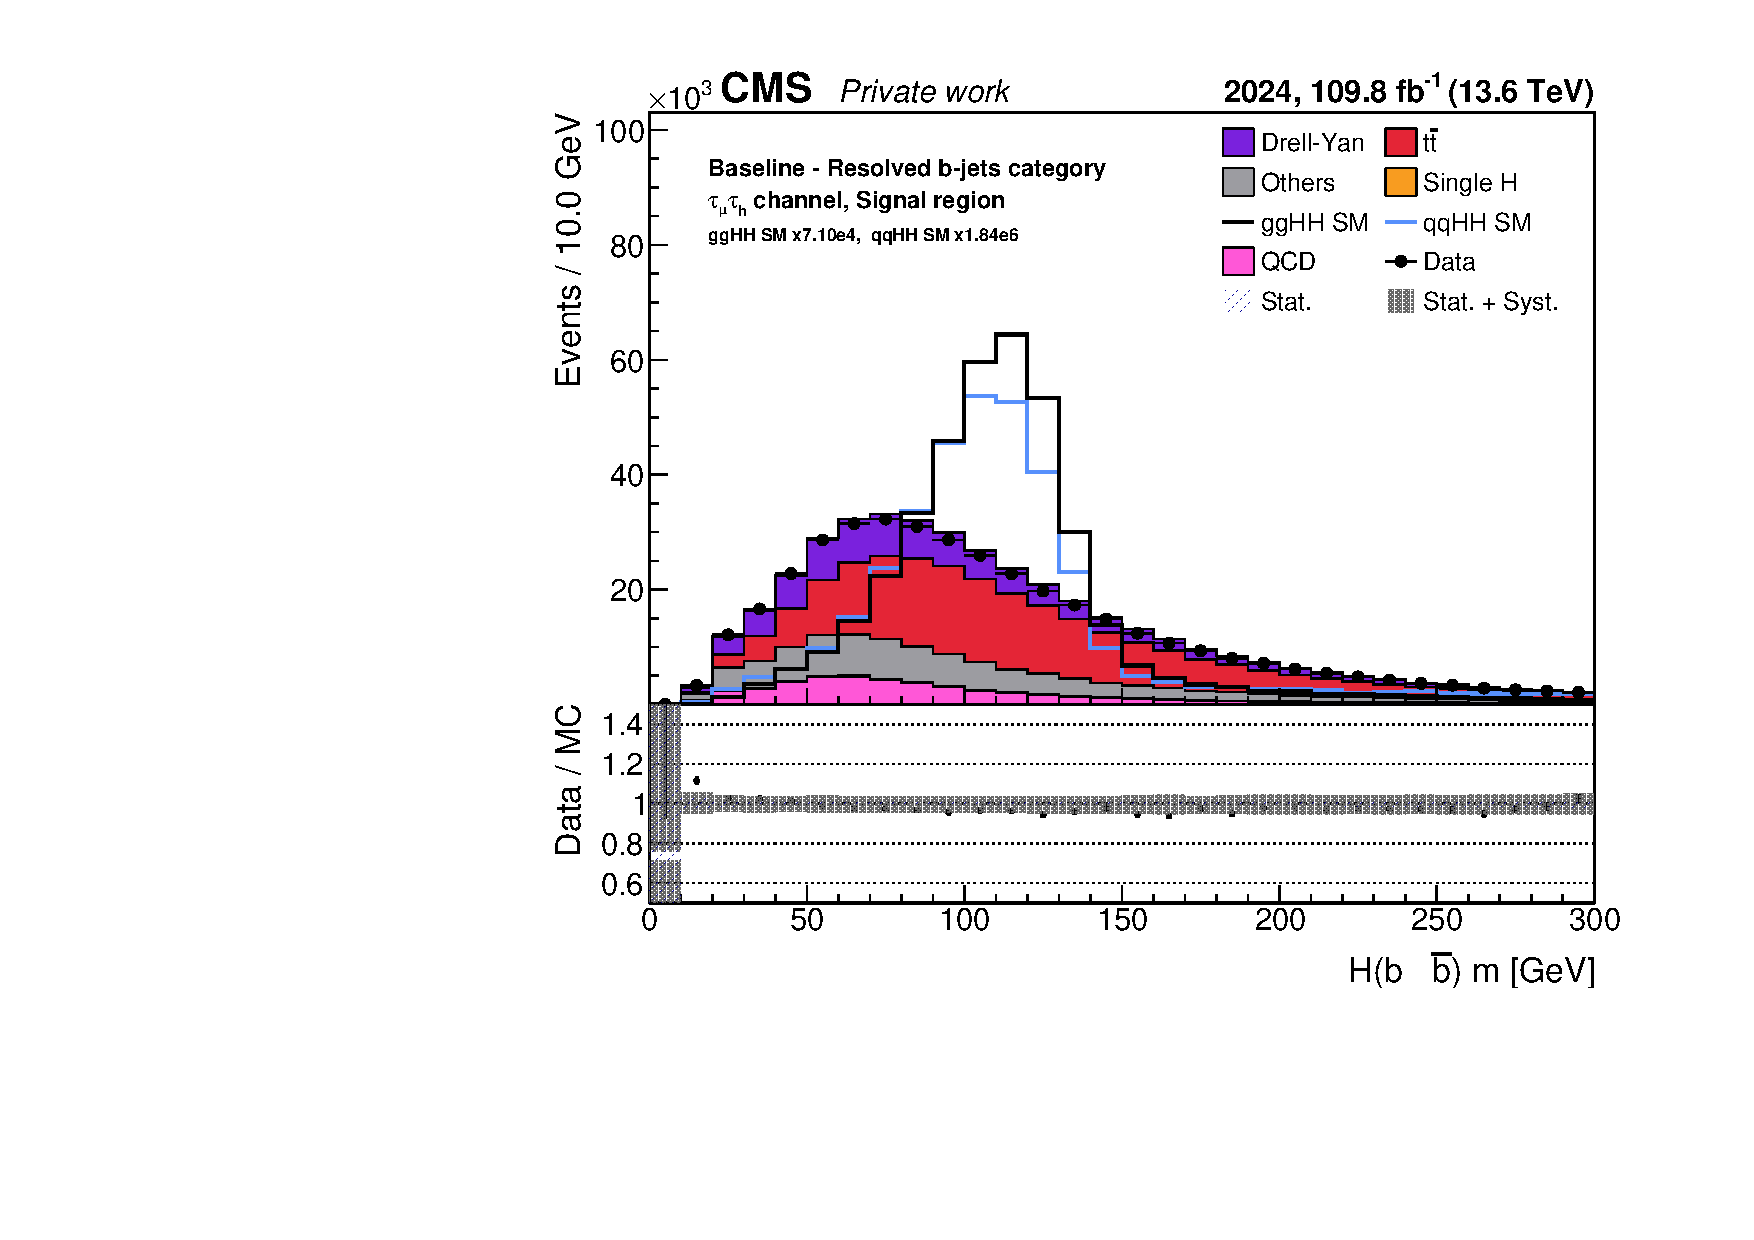
\includegraphics[width=0.5\linewidth, trim=11bp 0bp 40bp 14bp, clip]{figures/chapter_V/Hbb_mass__mutau_os_iso__pg_forPlots__qcd__stack__norm_sig.pdf}
    \caption[Reconstruction of the $b\bar{b}$ system mass]{Mass of the $H\to b\bar{b}$ candidate in the resolved topology, with the same selection and conventions as in Figure \ref{fig:htautau_mass}.}
    \label{fig:hbb_mass}
\end{figure}


\subsection{The VBF jets assignment}
%
In the final step of the object selection procedure, the VBF jets are assigned. Once the two Higgs boson candidates have been reconstructed, the event is examined to determine whether the jet configuration of the event is consistent with the jets characteristic of vector boson fusion production. The problem is solved with the \textsc{VBFjTag} algorithm (Section \ref{sec:VBFjTag}), used here for the first time in an analysis. Its score is evaluated over all the preselected jets with $|\eta| < 4.7$, including the two jets of the $H\to b\bar{b}$ candidate, which are flagged as such. The pair is then formed by the two jets with the highest scores among those that do not belong to the $H\to b\bar{b}$ candidate, which, when the candidate is boosted, excludes the jets within $\Delta R < 0.8$ of the large-radius jet.\medskip

% , about a quarter of the resolved selection in this channel, where $t\bar{t}$ production with additional radiation dominates the background and the simulation exceeds the data by about $8\%$, a difference in normalization that is nearly uniform in both variables except at the highest invariant masses.
% Así que no es que las variables VBF estén peor modeladas que $m_{\tau\tau}$. Lo que pasa es que esos plots seleccionan justo la parte de la muestra donde el MC sobreestima, la de sucesos con jets adicionales.

Figure \ref{fig:vbf_jets} shows the invariant mass and the pseudorapidity separation of the pair selected in this way, before any requirement on its kinematics. These observables are defined only for events with at least two jets in addition to the $H\to b\bar{b}$ candidate. In vector boson fusion, the two jets originate from the scattered quarks, emitted at small angles with respect to the beam in opposite hemispheres, so that the pair is separated by several units of pseudorapidity and reaches invariant masses above $1$ TeV. In gluon fusion and in the backgrounds, by contrast, the selected pair is formed by jets from radiation or from the decay of other particles, concentrated at small separations and masses. The identification of a pair is therefore not sufficient to classify an event as vector boson fusion, and additional requirements on these two variables are applied in the categorization, described below.
%
\begin{figure}[tbp]
    \centering
    \begin{subfigure}[b]{0.49\linewidth}
        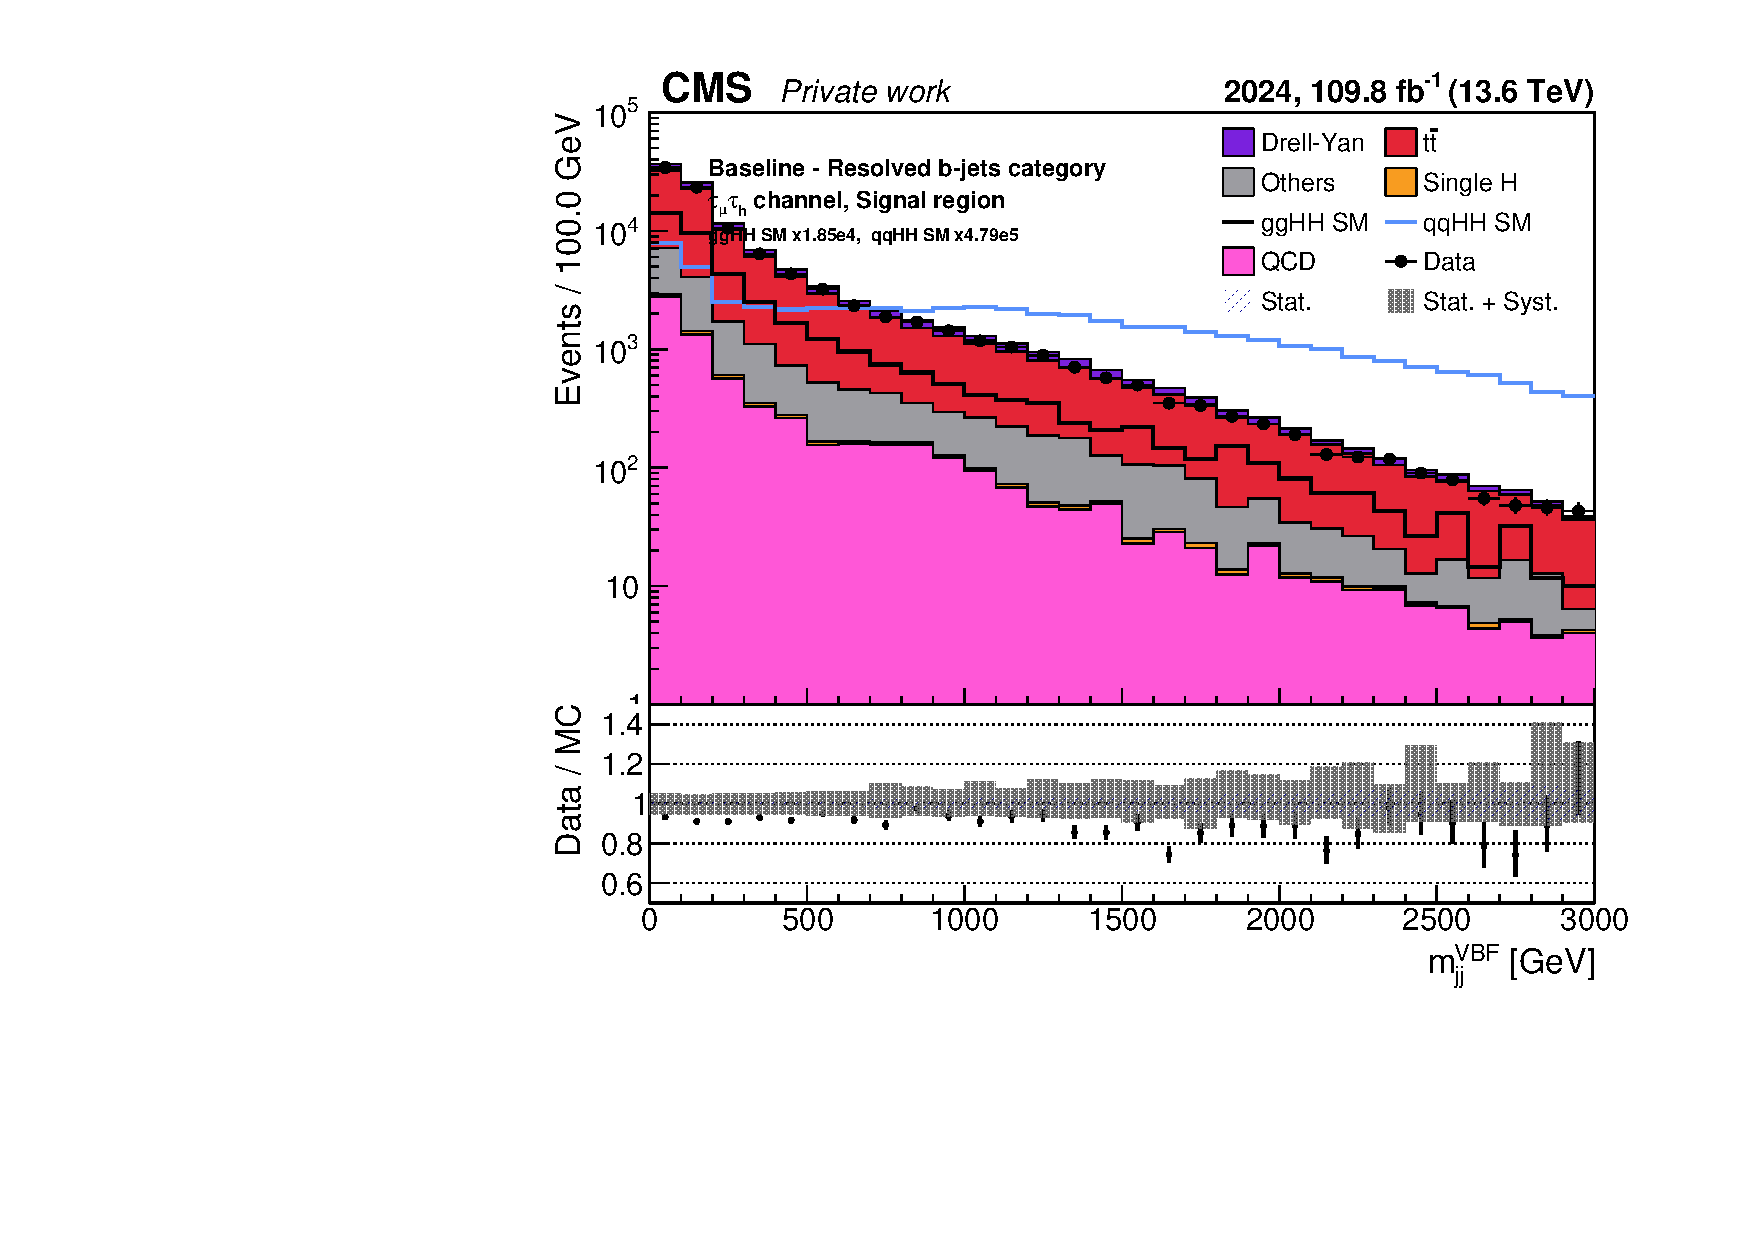
\includegraphics[width=\linewidth, trim=11bp 0bp 40bp 14bp, clip]{figures/chapter_V/VBFjj_mass_full__mutau_os_iso__pg_forPlots__qcd__stack__logY__norm_sig.pdf}
        \caption{Invariant mass}
        \label{fig:vbf_jets_mjj}
    \end{subfigure}
    \hfill
    \begin{subfigure}[b]{0.49\linewidth}
        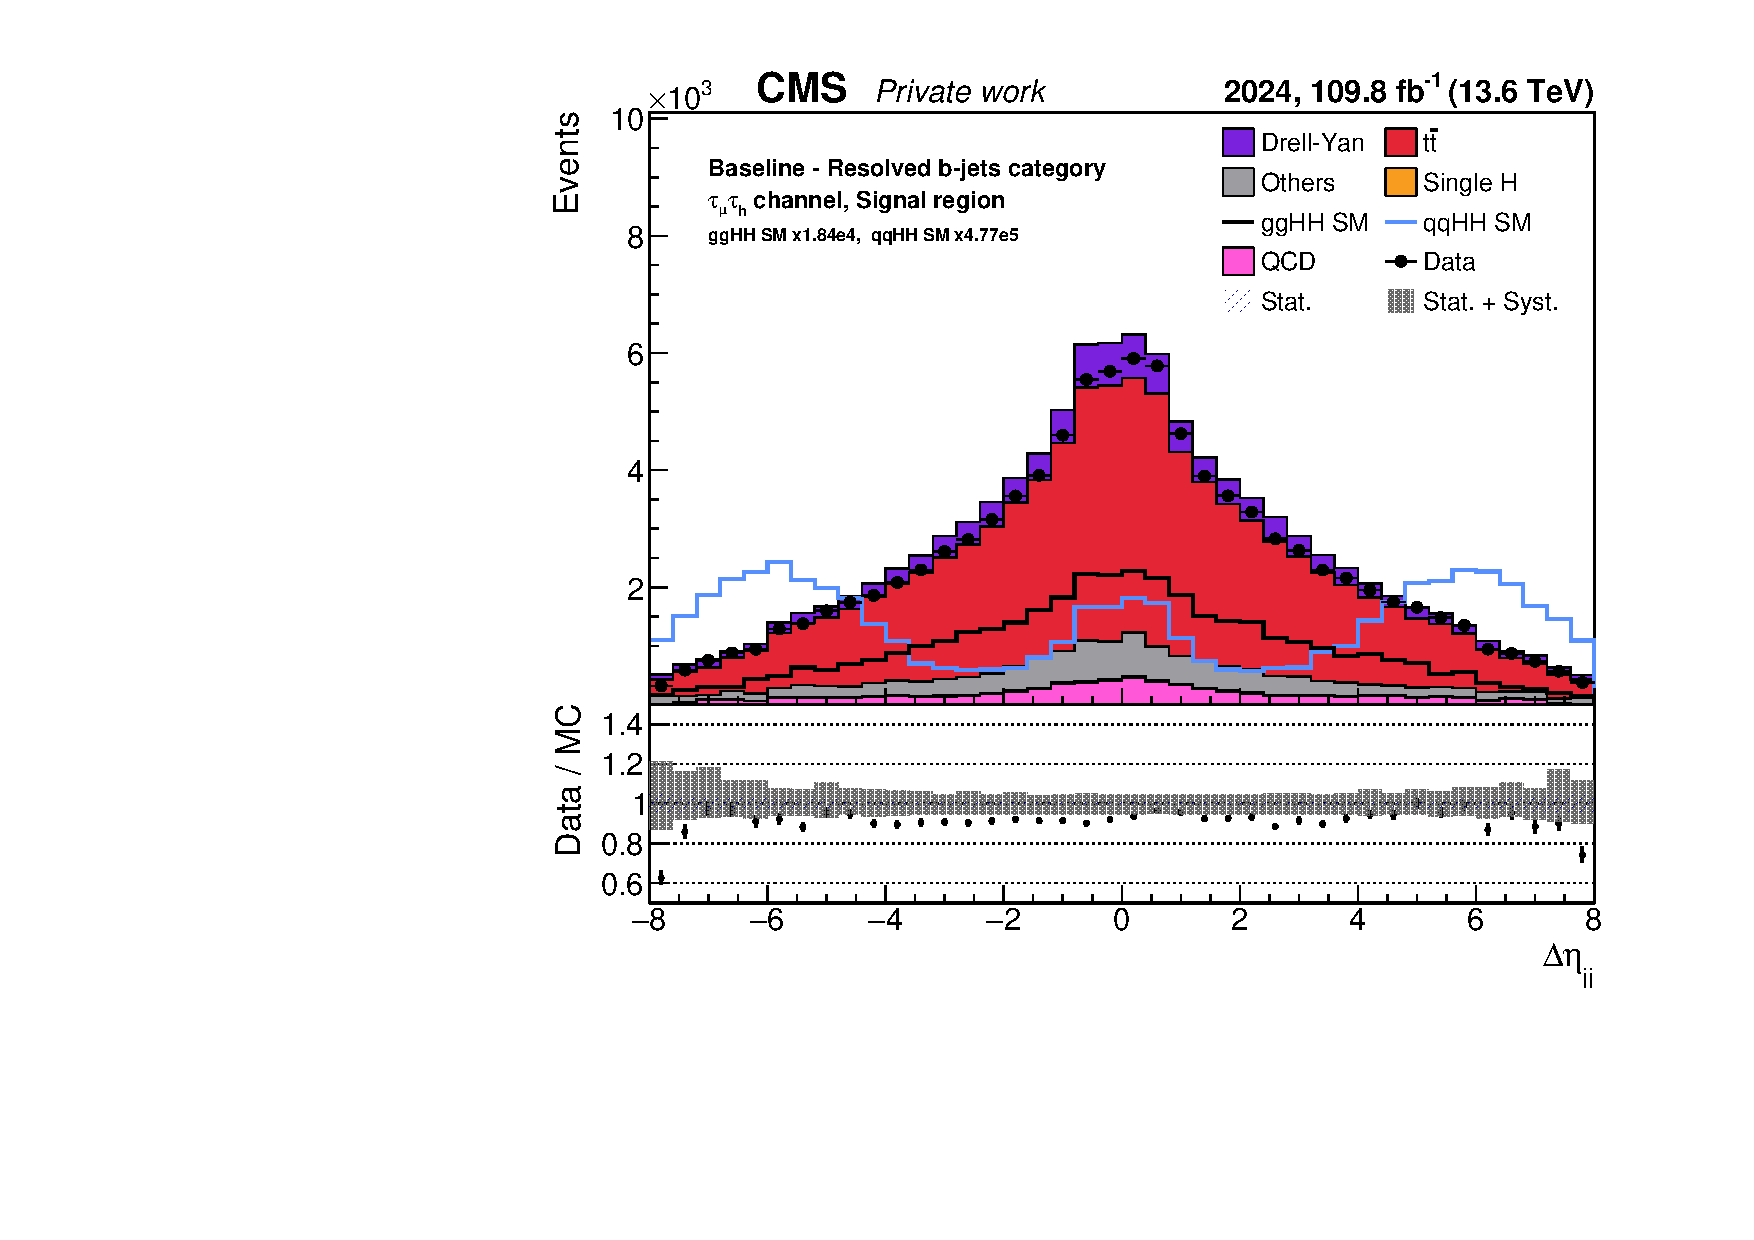
\includegraphics[width=\linewidth, trim=11bp 0bp 40bp 14bp, clip]{figures/chapter_V/VBFjj_deltaEta__mutau_os_iso__pg_forPlots__qcd__stack__norm_sig.pdf}
        \caption{Pseudorapidity separation}
        \label{fig:vbf_jets_deta}
    \end{subfigure}
    \caption[Kinematics of the VBF jet pair]{Invariant mass (a) and pseudorapidity separation (b) of the VBF jet pair, with no requirement on its kinematics and with the same selection and conventions as in Figure \ref{fig:htautau_mass}.}
    \label{fig:vbf_jets}
\end{figure}



\subsection{Event categorization}
% poner en algun sitio que está heredado del run 2 (y en qué puntos difiere), ya que en la linea472 si que estoy poniendo eso, pero esta descontextualizado
The steps described identify, in each event, the $H\to\tau\tau$ candidate, which determines the channel; the $H\to b\bar{b}$ candidate, reconstructed in the resolved topology, in the boosted topology, or in both; and, when present, the VBF jet pair. 

This description alone does not distinguish the signal from the background, since background events can yield the same reconstructed objects, and given the low cross section of Higgs boson pair production, the selected events are largely dominated by the background. The same low cross section prevents the signal from being extracted by tightening the selection, which would significantly reduce the signal, weaken the control of the background, and limit the analysis to specific signal hypotheses. Signal extraction therefore aims to preserve all information by dividing the events into mutually exclusive categories, which allow the phase space to be partitioned into regions with different signal-to-background ratios. In this manner, the overall sensitivity is enhanced precisely because the statistical fitting can exploit the contrast between categories, both in terms of composition and in the behavior of the discriminating variables.

The categories are defined on the reconstructed objects and examined in sequence, so that an event that does not satisfy the conditions of one category is examined for the next. One criterion is the channel defined by the $\tau\tau$ pair, and the other the topology of the event. It is first evaluated whether the $b\bar{b}$ system is collimated, which assigns the event to the boosted category, then whether it exhibits the topology of vector boson fusion, which assigns it to the VBF category, and the remaining events are distributed among resolved categories, subdivided according to the $b$ tagging of the two jets and subject to a selection in the $(m_{H\tau\tau}, m_{Hbb})$ plane. This order, shown in Figure \ref{fig:category_flow}, ensures that each event falls into only one category and follows the expected number of events in each of them, so that the less populated categories take precedence and are not absorbed by the more populated ones where they overlap in phase space. The scheme is largely inherited from the Run 2 analysis, and the differences stem from the added phase space and from the algorithms available in Run 3.

%
The distinction between vector boson fusion and gluon fusion events, whether boosted or resolved, is particularly relevant from a physical standpoint, since gluon fusion gives access to the trilinear self-coupling of the Higgs boson and vector boson fusion to the coupling of two Higgs bosons to two vector bosons. Isolating one from the other therefore allows each to contribute where it is most sensitive, which improves the constraints obtained on both couplings. The categories are described below grouped by production mode, rather than in the order in which they are examined.

\subsubsection{Gluon-gluon fusion categories}
%
The first category examined is the least populated of the four, $b\bar{b}$-boosted gluon fusion, which includes events in which the identified large-radius jet satisfies $p_T > 300$ GeV, $|\eta| < 2.5$, and a soft-drop mass between $80$ and $170$ GeV. Additionally, the large-radius jet must pass a custom \textsc{ParticleNet} threshold of $0.75$, optimized specifically for this analysis. Since it is defined only by the topology of the $H\to b\bar{b}$ candidate, this category also accepts events produced through vector boson fusion, but it is grouped with gluon fusion because this production mode dominates its signal content and its events are scored by the gluon fusion discriminant (Section \ref{sec:bbtt_extraction}).


% Additionally, the large-radius jet must pass a threshold of $0.75$ on the \textsc{ParticleNet}
% discriminant. In the absence of centrally calibrated working points for Run 3, this value was
% chosen by scanning thresholds between $0.1$ and $0.9$, repeating the full statistical analysis
% for each of them, and retaining the one that yields the best expected upper limit.


The events reconstructed in the resolved topology correspond to the last step in the chain, as shown in Figure \ref{fig:category_flow}. This category encompasses those events that do not fall into either the boosted category or the vector boson fusion category. To further enhance the sensitivity in this region, the events are divided into two categories based on the quality of the $b$ tagging for the two jets with the highest \textsc{HH-BTag} scores: resolved 2b, where both jets exceed the medium working point of the $b$ tagging discriminant, and resolved 1b, where only one of them does. This separation takes advantage of the fact that the purity of the two categories is very different, with the \textit{res2b} category being the most sensitive in the analysis while still retaining the statistical information provided by the \textit{res1b} region, which helps constrain the background normalizations in the fit.

For these resolved categories, the high statistics also allow for a further selection in the plane defined by the two reconstructed masses, as shown in Figure \ref{fig:mass_ellipse}. It should be noted that the purpose of this cut has evolved compared to Run 2, where the cut parameters were obtained by minimizing the background acceptance and where it was required to preserve more than $90\%$ of the signal. Since the discrimination between signal and background now rests entirely on the signal extraction neural network, the mass selection no longer aims to improve that ratio, but rather to delimit the complementary region, which is used as a sideband region to derive the $t\bar{t}$ background fake factors (Section \ref{sec:bbtt_ff}). The cut is defined as an ellipse in the $(m_{H\tau\tau}, m_{Hbb})$ plane, with parameters optimized separately for each channel to take advantage of the different resolutions of the objects involved, and fit to preserve $99\%$ of the signal:
%
\begin{align}
    \tau_\mu\tau_h &: \left(\frac{m_{H\tau\tau} - 110}{45}\right)^{2} + \left(\frac{m_{Hbb} - 118}{215}\right)^{2} \leq 1, \\
    \tau_e\tau_h   &: \left(\frac{m_{H\tau\tau} - 111}{38}\right)^{2} + \left(\frac{m_{Hbb} - 118}{225}\right)^{2} \leq 1, \\
    \tau_h\tau_h   &: \left(\frac{m_{H\tau\tau} - 130}{36}\right)^{2} + \left(\frac{m_{Hbb} - 125}{222}\right)^{2} \leq 1,
\end{align}
%
where all quantities are expressed in GeV. The ellipses are much narrower along $m_{H\tau\tau}$ than along $m_{Hbb}$, since it is in the former direction that the background is most widely distributed, and therefore where a narrow cut is most effective. No mass selection is applied in the boosted and VBF categories, where the statistics are already limited, nor in the res1b and res2b categories of the $b\tau_h\tau_h$ channel.
%fondo 56%
%
\begin{figure}[tbp]
    \centering
    \begin{subfigure}[b]{0.49\linewidth}
        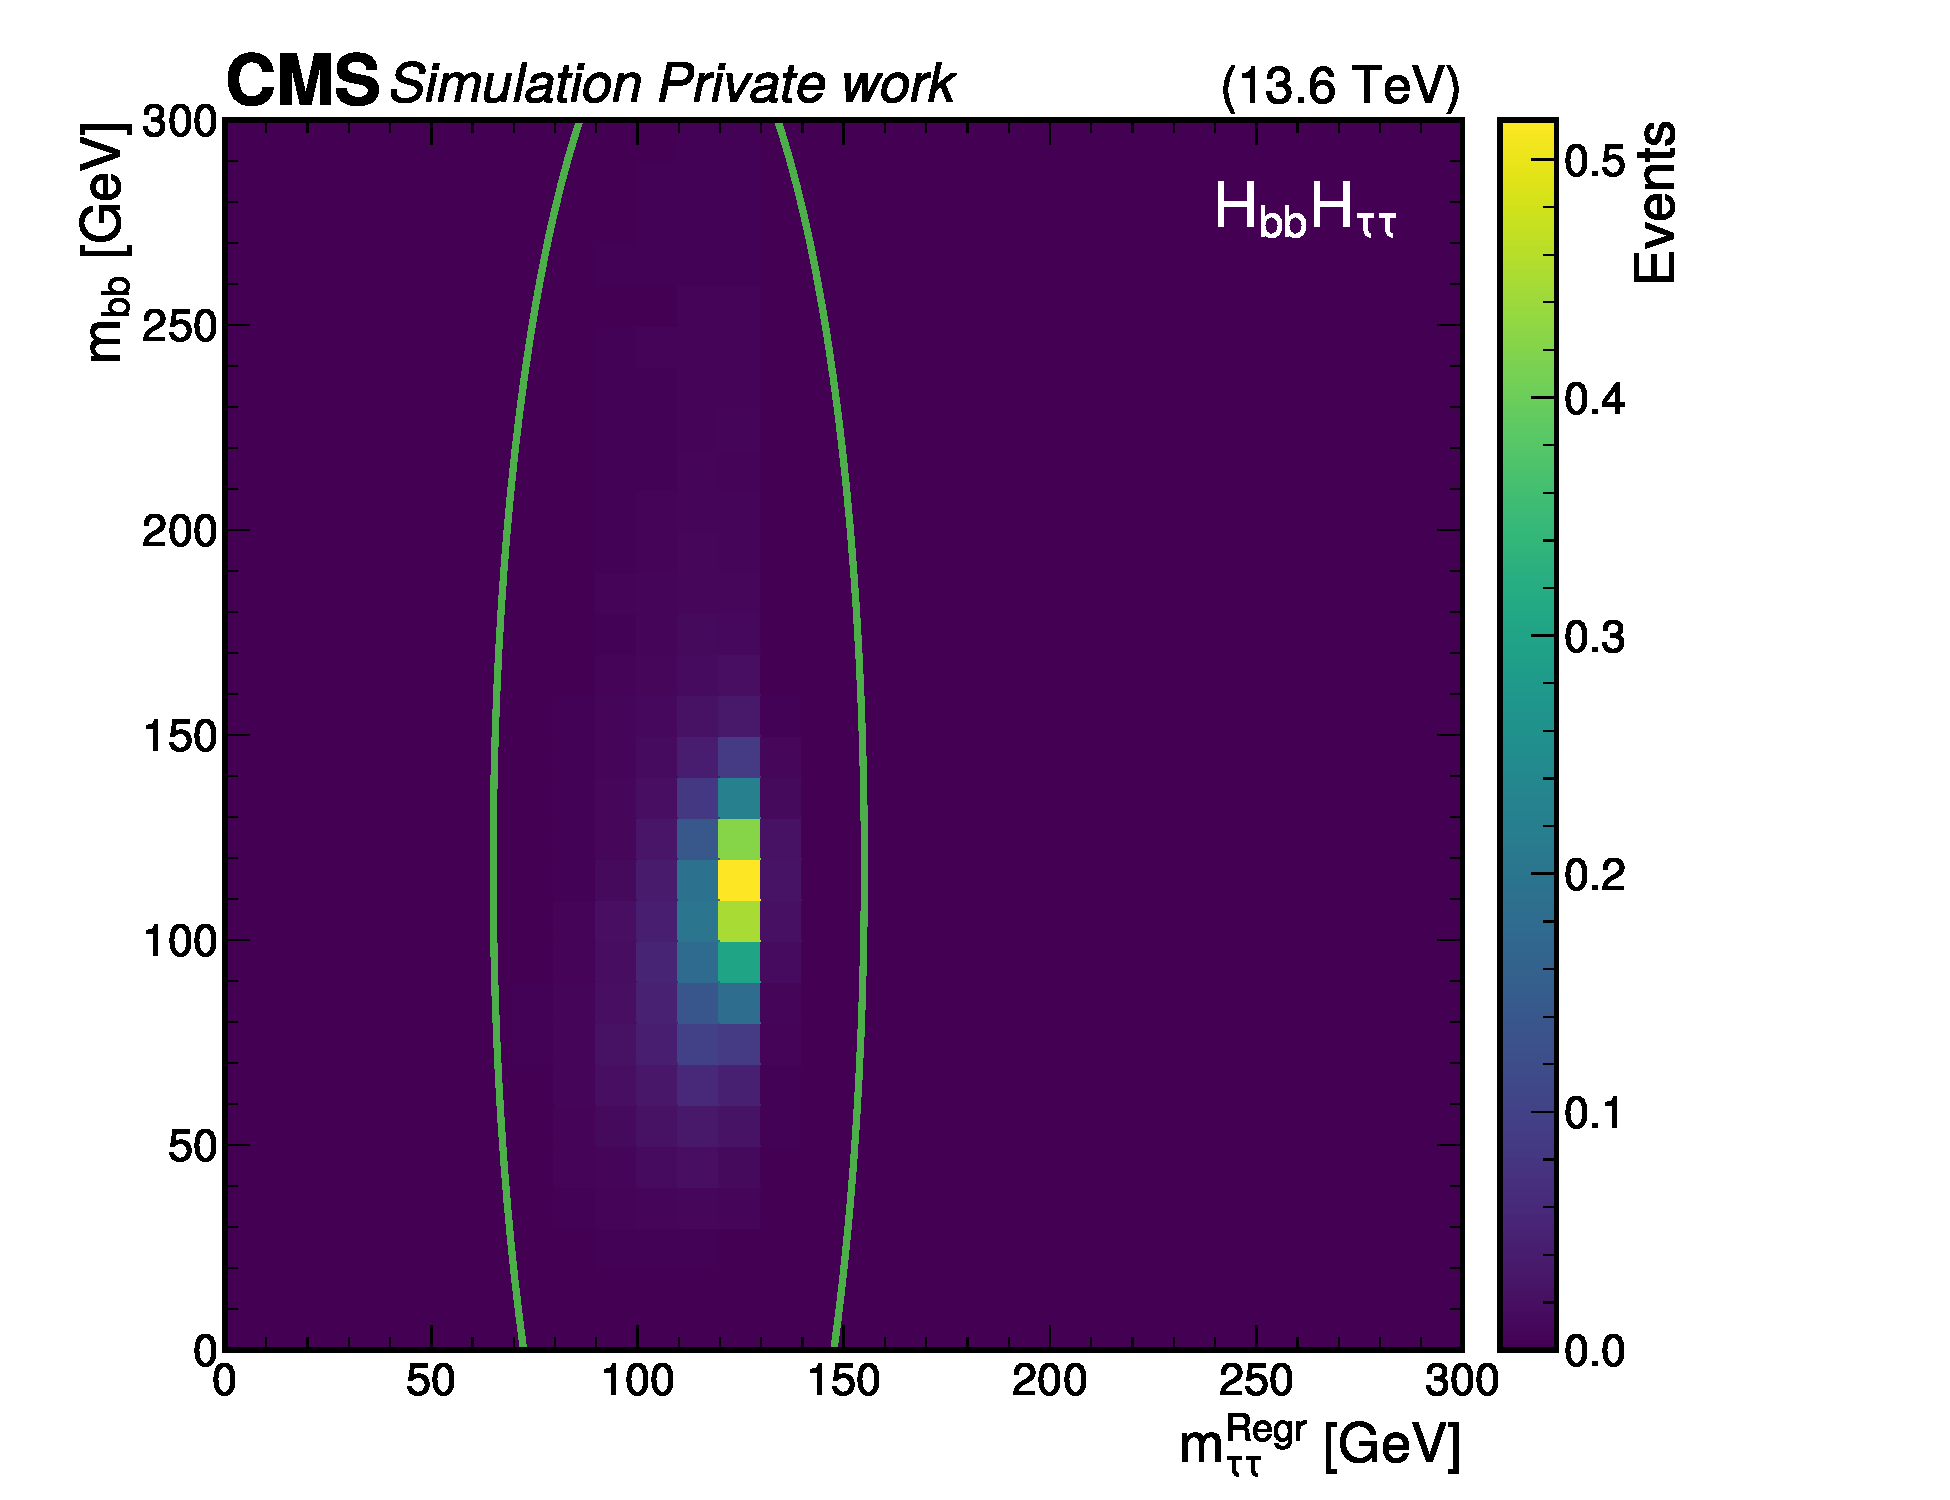
\includegraphics[width=\linewidth, trim=36bp 9bp 111bp 22bp, clip]{figures/chapter_V/masscut_mutau_sgn_Htt_regr_mass_res12b.pdf}
        \caption{Signal}
        \label{fig:mass_ellipse_sgn}
    \end{subfigure}
    \hfill
    \begin{subfigure}[b]{0.49\linewidth}
        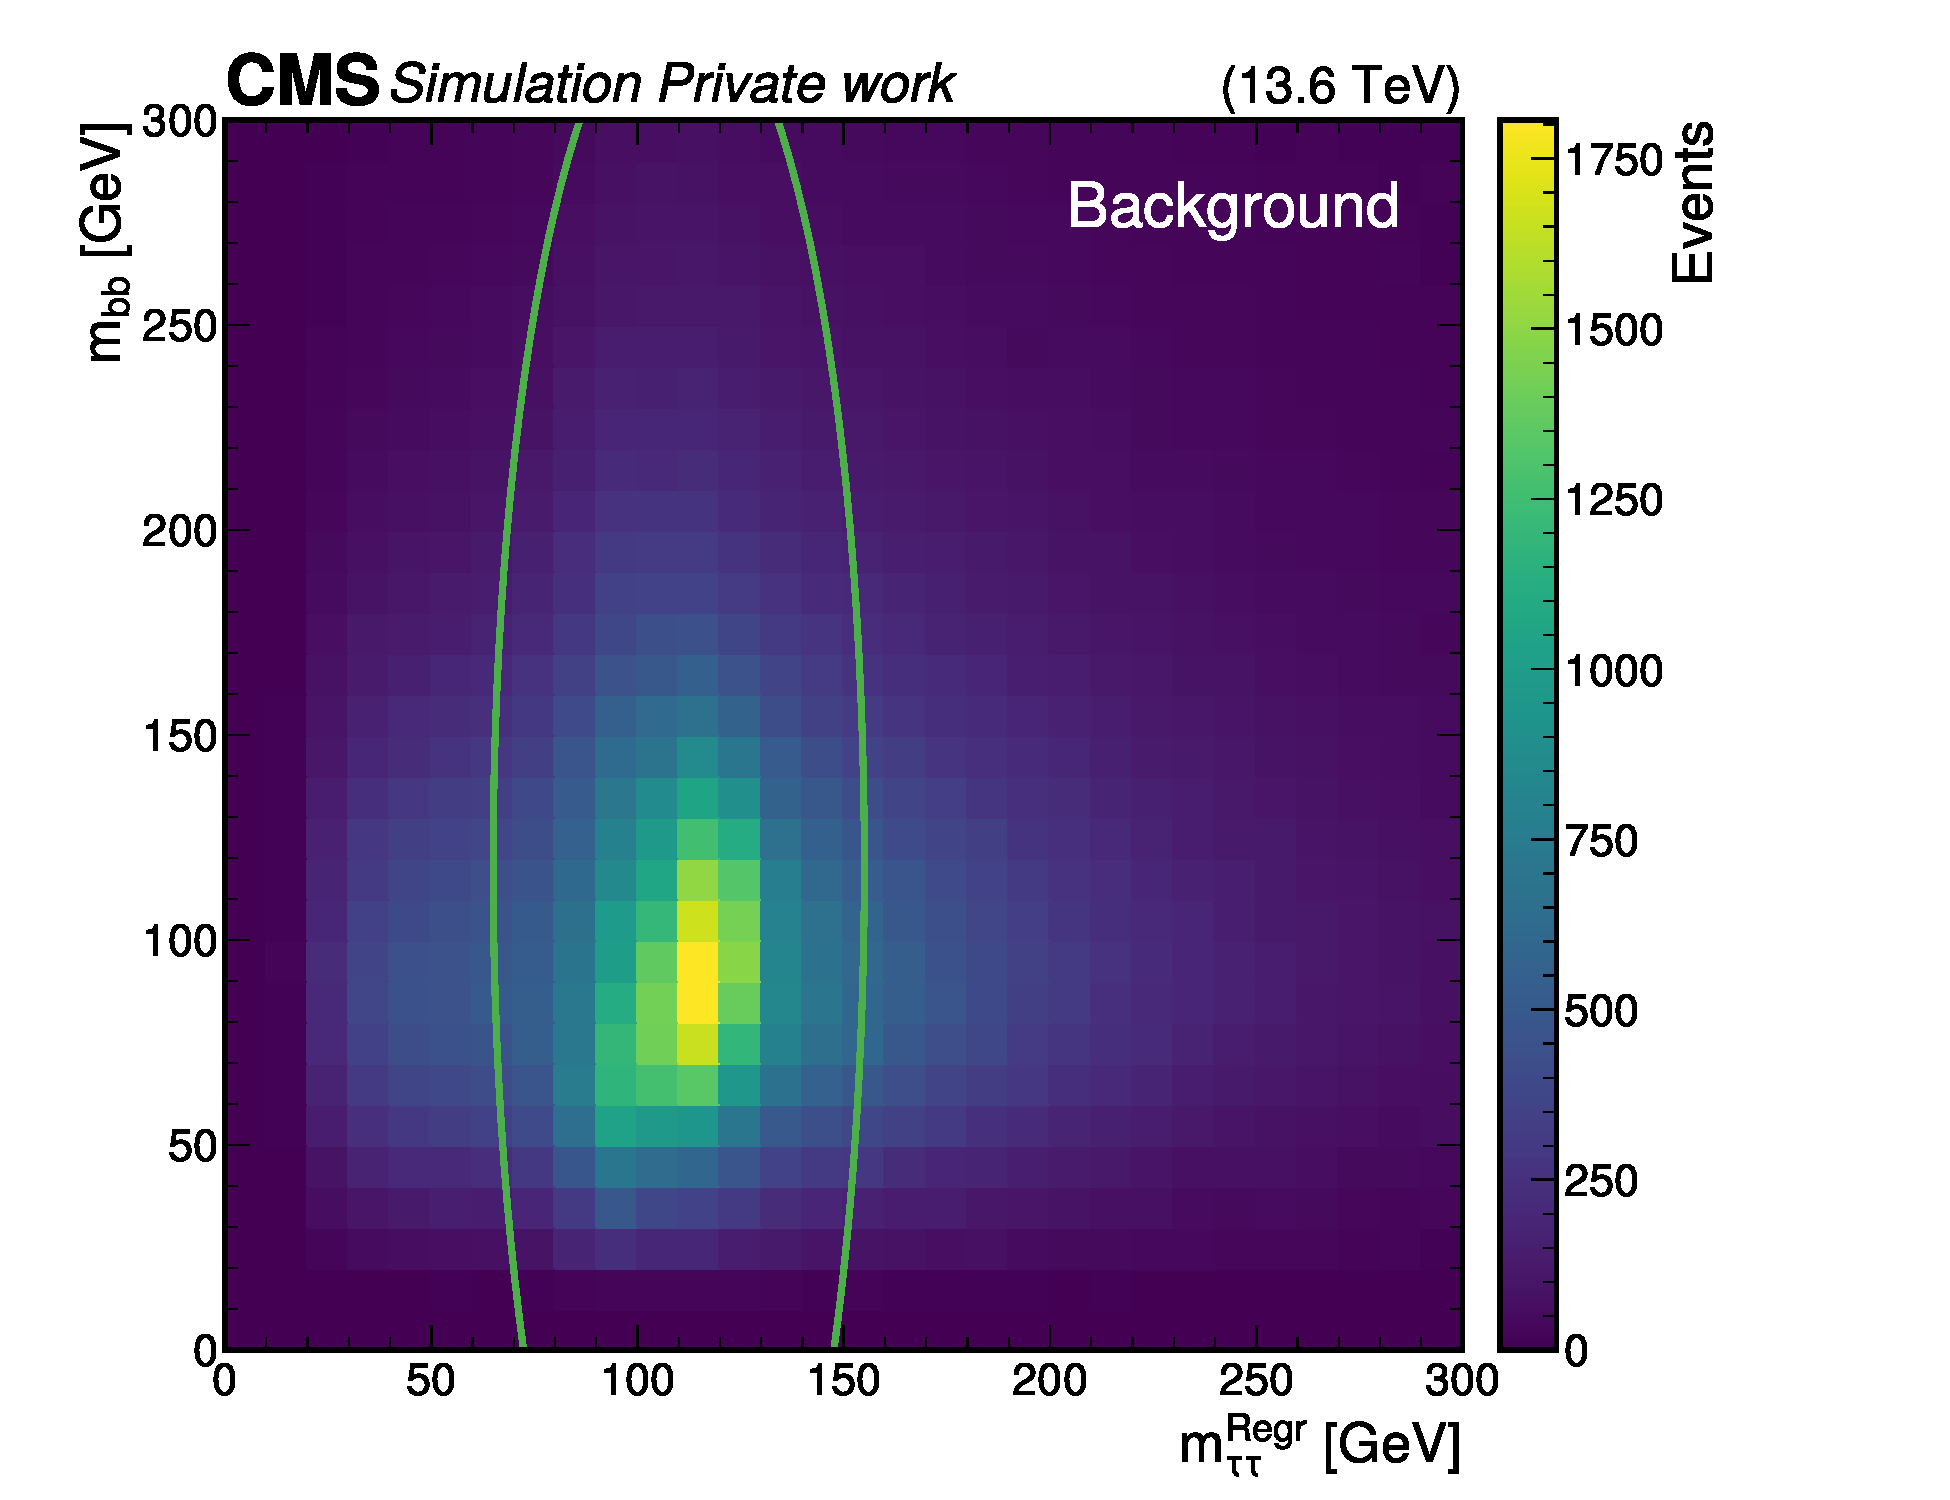
\includegraphics[width=\linewidth, trim=36bp 9bp 111bp 22bp, clip]{figures/chapter_V/masscut_mutau_bkg_Htt_regr_mass_res12b.pdf}
        \caption{Background}
        \label{fig:mass_ellipse_bkg}
    \end{subfigure}
    \caption[Elliptical mass selection]{Distribution of the reconstructed masses of the two Higgs boson candidates, $m_{bb}$ against the regressed $m_{\tau\tau}$, for the SM ggF and VBF $HH$ signal (a) and for the sum of the simulated backgrounds (b), in the res1b and res2b categories of the $\tau_\mu\tau_h$ channel before the mass selection. The green ellipse delimits the region retained by the mass selection.}
    \label{fig:mass_ellipse}
\end{figure}




\subsubsection{Vector boson fusion category}
%
What sets this category apart is the nature of what has to be rejected in it. In the gluon fusion categories the contaminant is the background; here it is, to a large extent, the other signal. Gluon fusion production is significantly more abundant, and events of that kind entering this region do not appear as an excess foreign to the process being sought, but as one indistinguishable from it, so that the category would lose the very ability that justifies its existence.

It is therefore situated at the midpoint of the chain flow, where events that have not been classified as boosted are examined to determine whether they exhibit the topology of a vector boson fusion before being redirected to the resolved categories. This requires the identification of a pair of VBF jets with an invariant mass greater than $500$ GeV and a pseudorapidity separation of $\Delta\eta_{jj} > 3.0$; these kinematic cuts are defined to achieve the best balance between acceptance and background contamination\footnote{While the trigger paths allow events up to $\Delta\eta_{jj} > 2.5$, the specific study in this phase space has shown that relaxing the selection to that value significantly increases the contamination from gluon-gluon fusion production without improving the expected sensitivity in the category}. The selected pair must also be accompanied by a resolved $H\to b\bar{b}$ candidate where at least one of its two jets passes the medium working point of the $b$ tagging discriminant. This last condition ensures that the category isolates $HH$ production via vector boson fusion, rather than merely selecting dijet configurations that resemble the VBF topology but do not contain a Higgs boson. Once isolated, the VBF events are not further subdivided, owing to their reduced statistics. In Run 2, they were distributed among several subcategories by a multiclass neural network~\cite{CMS-HIG-20-010}, whereas here this separation is left to the dedicated discriminant described in Section \ref{sec:bbtt_extraction}.


%INVENTADO: [...] y de ahí también que, una vez aislada, no se subdivida. En Run 2 esta región se repartía a su vez en subcategorías asociadas a procesos concretos; ahora esa separación la realiza de forma continua la distribución de salida de la red con la que se extrae la señal, de manera que un reparto explícito no añadiría información.


\subsubsection{Signal regions}
%
The four categories defined in this way — boosted, VBF, res1b, and res2b — are in principle evaluated for each of the four final states of the $\tau\tau$ pair — $\tau_\mu\tau_h$, $\tau_e\tau_h$, $\tau_h\tau_h$, and $b\tau_h\tau_h$. However, owing to the limited number of events in the boosted and VBF categories, their four final states are merged into a single one, denoted $X\tau_h$, so that the scheme consists of the ten categories shown in Figure \ref{fig:categories}. In each of them, the signal region is finally obtained by imposing the two conditions left unapplied throughout the selection, that the two $\tau$ candidates have opposite charges and that the $\tau_h$ candidate passes the Medium WP of the discriminant against jets. Applied across the five data-taking periods, the analysis therefore explores fifty signal regions simultaneously in the statistical fit described in Section \ref{sec:bbtt_statistics}.
%
\begin{figure}[tbp]
\centering
\definecolor{recBg}{HTML}{F1F6FC}\definecolor{recLn}{HTML}{9BBDE3}
\definecolor{catBg}{HTML}{ECF7F5}\definecolor{catLn}{HTML}{72B9B1}
\definecolor{outBg}{HTML}{F2F2F4}\definecolor{outLn}{HTML}{AEAEB8}
\definecolor{srABg}{HTML}{E4F3E6}\definecolor{srALn}{HTML}{86C28F}
\definecolor{srBBg}{HTML}{F1F8E4}\definecolor{srBLn}{HTML}{B3D27E}
\newcommand{\ffont}{\fontfamily{Nunito-TLF}\selectfont}
\begin{tikzpicture}[
    x=1mm, y=1mm, font=\ffont\footnotesize,
    chip/.style  = {draw=outLn, line width=0.5pt, rounded corners=2pt, fill=outBg,
                    inner sep=1pt, minimum height=7mm, minimum width=20mm},
    res/.style   = {draw=outLn, line width=0.6pt, rounded corners=3pt, fill=outBg,
                    inner sep=1pt, minimum height=7mm, minimum width=26mm, font=\ffont\footnotesize\bfseries},
    cell/.style  = {draw=#1Ln, line width=0.6pt, rounded corners=3pt, fill=#1Bg,
                    align=center, inner sep=1pt, minimum width=26mm},
    num/.style   = {circle, fill=#1, text=white, font=\ffont\tiny\bfseries,
                    inner sep=0pt, minimum size=3.6mm},
    axis/.style  = {font=\ffont\scriptsize\bfseries, text=#1!75!black, inner sep=1.5mm},
    rule/.style  = {draw=#1, line width=0.6pt}
  ]
  % column headers: categories (steps 4-6)
  \foreach \x/\t/\n in {38/boosted/h1, 66/VBF/h2, 94/res2b/h3, 122/res1b/h4}
    \node[res] (\n) at (\x,0) {\t};
  \foreach \n/\k in {h1/4, h2/5, h3/6, h4/6}
    \node[num=catLn, anchor=center] at ([xshift=-1pt,yshift=-1pt]\n.north east) {\k};
  % row headers: channels (step 1)
  \foreach \y/\t/\n in {-10/{$\tau_\mu\tau_h$}/r1, -19/{$\tau_e\tau_h$}/r2,
                        -28/{$\tau_h\tau_h$}/r3, -37/{$b\tau_h\tau_h$}/r4}
    \node[chip] (\n) at (10,\y) {\t};
  % merged boosted and VBF signal regions
  \node[cell=srA, minimum height=34mm] at (38,-23.5) {$X\tau_h$\\boosted};
  \node[cell=srA, minimum height=34mm] at (66,-23.5) {$X\tau_h$\\VBF};
  % resolved signal regions, one per channel
  \foreach \y/\c in {-10/{$\tau_\mu\tau_h$}, -19/{$\tau_e\tau_h$},
                     -28/{$\tau_h\tau_h$}, -37/{$b\tau_h\tau_h$}}{
    \node[cell=srB, minimum height=7mm] at (94,\y)  {\c{} res2b};
    \node[cell=srB, minimum height=7mm] at (122,\y) {\c{} res1b};
  }
  % axis titles with rules spanning the headers
  \node[axis=catLn] (catax) at (80,7.5) {CATEGORY};
  \draw[rule=catLn] (h1.west |- catax) -- (catax.west);
  \draw[rule=catLn] (catax.east) -- (h4.east |- catax);
  \node[axis=recLn, rotate=90] (chax) at (-3,-23.5) {CHANNEL};
  \node[num=recLn, rotate=90] (chnum) at ([yshift=3mm]chax.east) {1};
  \draw[rule=recLn] (chnum.east) -- (chnum.east |- r1.north);
  \draw[rule=recLn] (chax.west) -- (chax.west |- r4.south);
  \draw[rule=recLn] (chax.east) -- (chnum.west);
\end{tikzpicture}
\caption[Signal regions]{Signal regions of the analysis, obtained by combining the channels defined in step 1 of Figure \ref{fig:category_flow} (rows) with the categories defined in steps 4 to 6 (columns).}
\label{fig:categories}
\end{figure}




This defines the set of regions over which the measurement is performed. However, extracting the signal requires determining the expected background levels in each region. As previously outlined, the vast majority of the background prediction comes from the simulation, which must first be corrected for the residual differences with respect to the data, as described in Section \ref{sec:bbtt_corrections}. The exception is the contribution of jets misidentified as $\tau_h$, which is not reliably described by the simulation, and therefore it is estimated from the data, as described in Section \ref{sec:bbtt_ff}.

% To this end, the conditions that have deliberately been left loose throughout this section are precisely the ones to be considered: the loose working point used to identify the $\tau_h$, the absence of any requirement regarding the relative charge of the pair, and the complementary region of the elliptic mass cut. Therefore, the intention behind these decisions was to delineate regions enriched in the background of interest and devoid of signal. The following section describes the modeling of each background contribution.

\section{Corrections to simulated events}
\label{sec:bbtt_corrections}
%
The processes that populate the regions defined in the previous section, along with the generators used to simulate them, were listed in Section \ref{sec:bbtt_samples}. Although the simulated samples are reconstructed using the same algorithms as the data, the simulation is unable to accurately reproduce either the conditions under which the data were collected or the detector response to each object. There are also known shortcomings in the generator that affect the description of the $p_T$ in the two dominant backgrounds of the analysis, Drell--Yan and $t\bar{t}$, and which must be corrected. Therefore, correction factors or scale factors are introduced into the simulated events to improve the agreement between the data and the simulation. The scale factors act in two ways: some weight each event according to its characteristics, which changes the expected number of events of the sample; others modify the four-momentum of specific objects, which changes their distributions and, since objects can then cross the selection thresholds, also the number of selected events.

In many cases, these corrections are derived centrally in CMS and are common to all analyses. However, there are others that depend on trigger paths, objects, or phase spaces specific to this search, and which are in consequence derived and validated within the analysis itself. All correction factors applied to the simulated events are described below, and their associated uncertainties are described in Section \ref{sec:bbtt_systematics}.


%The processes that populate the regions defined in the previous section, along with the generators used to simulate them, were listed in Section \ref{sec:bbtt_samples}. However, the method for obtaining the expected number of events in each region has not yet been explained. This method does not simply amount to normalizing these samples to the integrated luminosity, but rather requires further considerations depending on the process and the origin of the $\tau_h$ candidate. As previously noted, events in which both $\tau$ leptons are genuine are taken directly from the simulation. However, the simulation of the two main contributions, Drell--Yan and top quark pair production, shows known discrepancies with respect to the data, necessitating corrections to the simulation. Additionally, the contribution from those events in which a hadronic jet has been erroneously identified as $\tau_h$ — which will simply be referred to as \textit{fakes} hereafter — cannot be reliably described using MC simulation, and therefore, it is estimated directly from the data.

\subsection{Object-level corrections}
\label{subsec:bbtt_object_corrections}
%
The corrections included in this subsection do not depend on the simulated physical process, but solely on the objects present in the event and the conditions under which the event was recorded. These corrections therefore apply equally to all simulated samples, including the signal. Most of the corrections introduced here address an efficiency — whether of a trigger path or an identification criterion — via a scale factor defined as the ratio between the efficiency measured in the data and that obtained in simulation. These efficiencies are commonly measured using the tag-and-probe method, which exploits a well-known resonance, typically the $Z$ boson, to define, based on its decay products, the \textit{tag} — which must satisfy tight selection criteria that ensure the purity of the sample — and the \textit{probe} — used to measure the efficiency of the criterion under study without biasing it. The remaining corrections affect the energy scale and resolution of the reconstructed objects. %All of them arise as an event progresses through the analysis: first, the pileup conditions under which it was recorded; then, its selection by the trigger; and finally, the reconstruction and identification of each of the objects in its final state.

%
\subsubsection{Pile-up reweighting}
%
The pile-up profile is set in advance for each simulation campaign based on the expected running conditions of the LHC. However, the profile actually recorded differs from this, and since pile-up affects the detector response and, to an extent that depends on the object, its reconstruction, this discrepancy must be corrected. Following the procedure recommended for Run 3, each simulated event is weighted according to the ratio of the distribution of the number of interactions in the data to that in the simulation.



\subsubsection{Trigger efficiency scale factors}
%
The trigger selection is applied equally to data and simulation, but its efficiency may differ between the two, and it is corrected with scale factors evaluated event by event as the ratio of the efficiencies measured in data and in simulation. For the single-lepton triggers and for the lepton and $\tau_h$ legs of the cross triggers, these efficiencies are provided centrally as a function of the $p_T$ of the object and, for $\tau_h$, of its decay mode. In the semileptonic channels, where the logical OR of both triggers is used, its efficiency is obtained by adding the efficiency of the single-lepton trigger and that of the cross trigger, and subtracting the overlap between the two. Each of these terms is built from the efficiencies of the individual legs, under the assumption that the lepton and $\tau_h$ legs are uncorrelated.\medskip

The triggers introduced in Run 3 and described in Section \ref{sec:triggers} lack central calibrations, and their scale factors are therefore measured within the analysis. This is the case for the jet leg of DiTau+Jet, for the $p_T^\text{miss}$ trigger, for the $\tau\tau$-tagging component of the large-radius jet trigger — whose jet component is taken from the corresponding Run 3 search in the $4b$ final state — for the VBF triggers, and for the QuadJet parking trigger. All of them follow the same approach. Each trigger is split into components that can be measured separately, and the efficiency of each is determined in data and simulation using a reference trigger that does not bias it, typically a single-lepton trigger or one sharing the remaining requirements. The QuadJet trigger, introduced in 2024 for the $\tau_h\tau_h$ final state and whose scale factors were derived as part of this thesis, is described below as a representative example

At the HLT, this trigger requires at least four jets with $p_T > 25$ GeV and $H_T > 250$ GeV, where $H_T$ is the scalar sum of the jet $p_T$, with one jet passing an online \textsc{ParticleNet} $b$ tagging requirement and another an online \textsc{ParticleNet} $\tau_h$ identification requirement. At Level-1, among the seeds that feed the path, the analysis requires the one with $H_T > 280$ GeV, computed from the Level-1 jets. Accordingly, its efficiency is broken down into these elements, with the $H_T$ requirement split into its Level-1 and HLT components,
%
\begin{equation}
    \varepsilon_\text{QuadJet} = \varepsilon_{H_T}^\text{L1}\cdot\varepsilon_{H_T}^\text{HLT}
    \cdot\varepsilon_{b}\cdot\varepsilon_{\tau_h}.
    \label{eq:quadjet_eff}
\end{equation}
%

Each factor is measured in data and simulation in a region enriched in the corresponding objects. The $\tau_h$ leg is measured in $Z\to\tau\tau\to\mu\tau_h$ events selected with a single-muon trigger, with a visible mass between $40$ and $80$ GeV and $m_T < 30$ GeV to suppress $W$+jets, as a function of the $p_T$ and $\eta$ of the $\tau_h$. The two $H_T$ components are measured in the same region as a function of $H_T$, and the $b$ tagging leg in $t\bar{t}$ events selected with an $e\mu$ trigger, as a function of the $b$ tagging score of the leading tagged jet. The $H_T$ scale factors, shown in Figure \ref{fig:quadjet_sf}, depart most from unity below $H_T = 400$ GeV, where the Level-1 requirement is still in its turn-on, so this threshold is imposed offline in the region where the trigger is used.}
%
\begin{figure}[tbp]
    \centering
    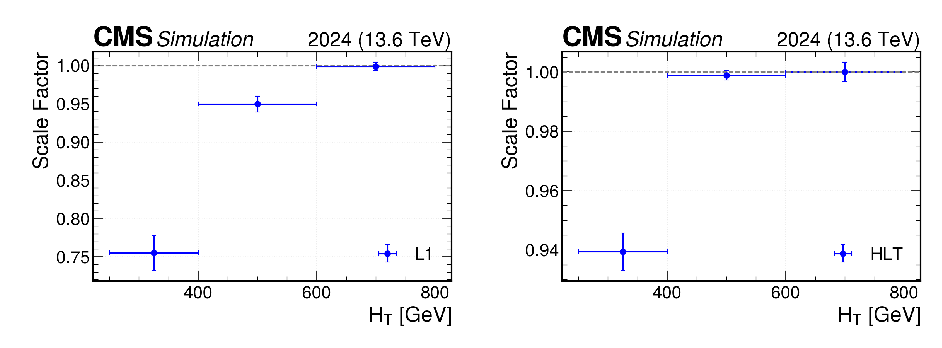
\includegraphics[width=\linewidth]{figures/chapter_V/quadjet_trigger_sf_HT.pdf}
    \caption[QuadJet trigger scale factors for the $H_T$ requirement]{%
        Scale factors of the Level-1 (left) and HLT (right) $H_T$ requirements of the QuadJet
        parking path, as a function of $H_T$, for the 2024 data-taking period.}
    \label{fig:quadjet_sf}
\end{figure}

The factorization relies on two simplifications whose combined effect must be checked. First, it neglects possible correlations between the components. Second, the $\tau_h$ and $b$ tagging efficiencies are evaluated only for the leading $\tau_h$ and $b$ jet candidates, which are the ones required to match the trigger objects in the analysis, whereas the trigger may also have been fired by the subleading ones. The factorized efficiency therefore misses this fraction of the events and is expected to underestimate the true one. Both effects are tested in simulated ggF signal events of the $\tau_h\tau_h$ channel with $H_T > 400$ GeV, by comparing the efficiency obtained from Equation \ref{eq:quadjet_eff} with the fraction of events that fire the trigger. The comparison is shown in Figure \ref{fig:quadjet_closure} as a function of the $p_T$ of the leading $b$ jet, a variable on which none of the factors is parameterized, so that the closure is not satisfied by construction. The factorized efficiency is systematically lower, by up to about $15\%$, and this non-closure is assigned as an additional uncertainty.
%
\begin{figure}[tbp]
    \centering
    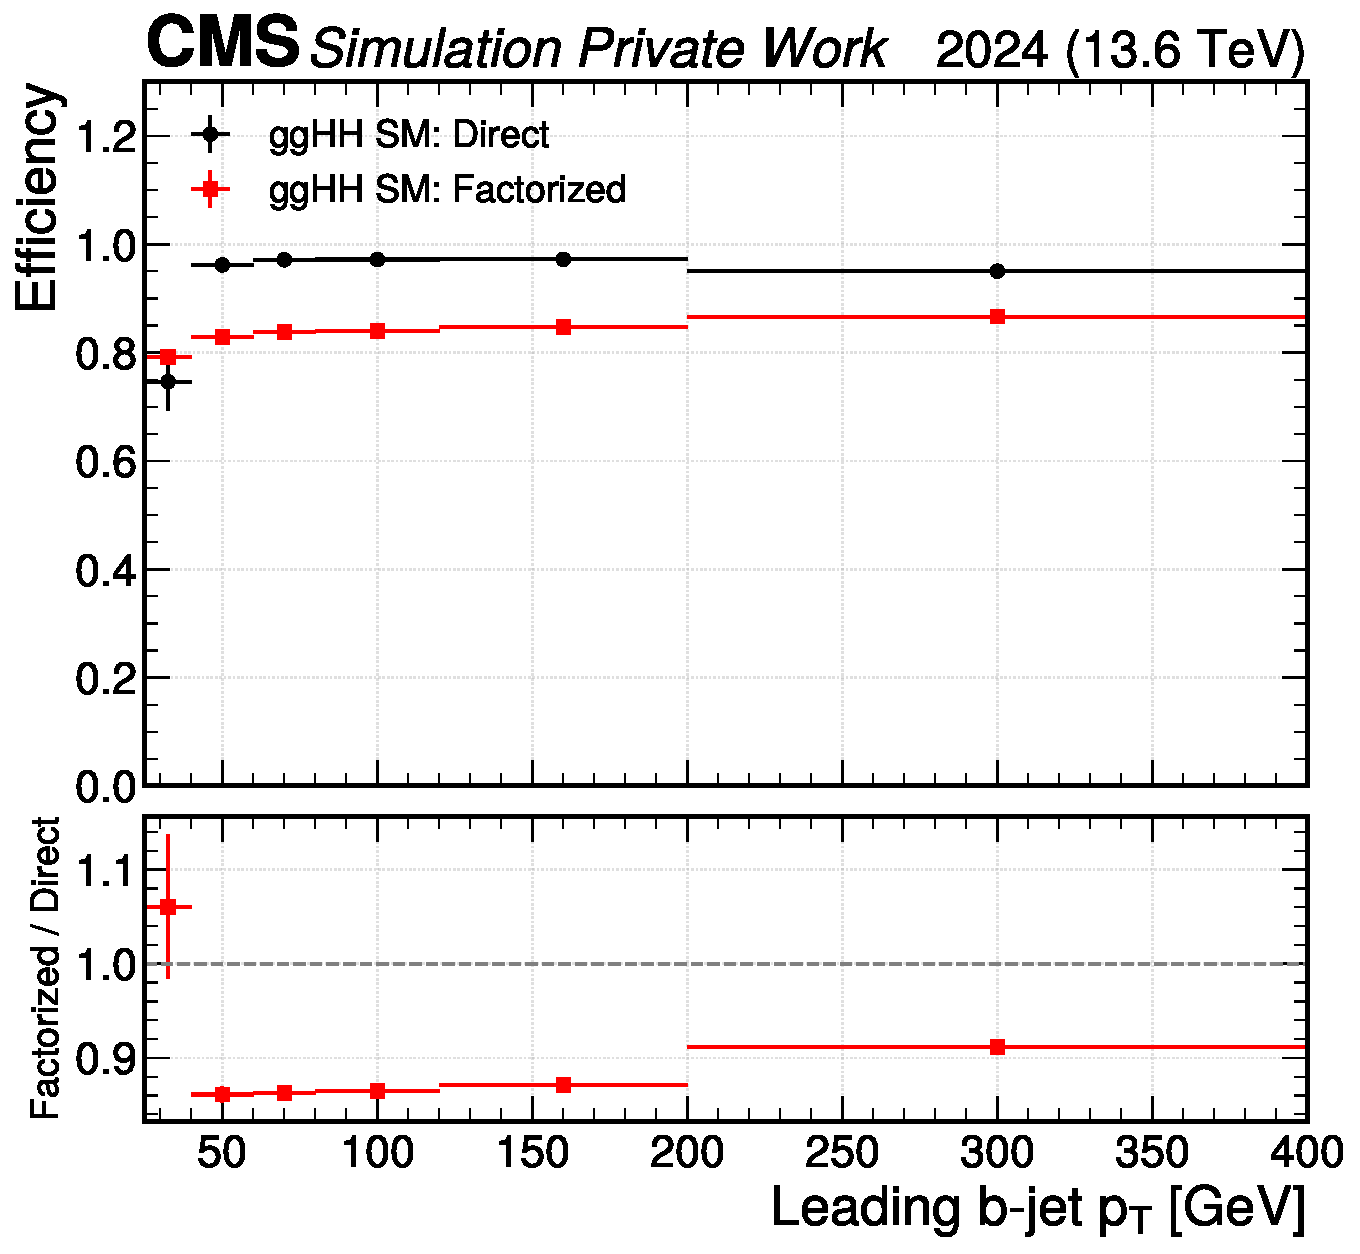
\includegraphics[width=0.5\linewidth]{figures/chapter_V/closure_1d_vs_bjet1pt_shortlegend.pdf}
    \caption[Closure of the factorized QuadJet trigger efficiency]{%
        Efficiency of the QuadJet parking trigger in simulated ggF signal events of the
        $\tau_h\tau_h$ channel with $H_T > 400$ GeV, as a function of the $p_T$ of the leading
        $b$ jet, measured directly (black) and obtained from the product of the factorized
        components evaluated on the leading $\tau_h$ and $b$ jet candidates (red), with their
        ratio in the lower panel.}
    \label{fig:quadjet_closure}
\end{figure}


\subsubsection{Muons and electrons}
%
The identification and isolation efficiencies of muons are corrected with scale factors derived centrally with the tag-and-probe method on $Z\to\mu\mu$ events. For electrons, the analogous factors, derived on $Z\to ee$ events, correct separately the reconstruction efficiency and the identification and isolation efficiency. Electrons also receive energy scale and resolution corrections, obtained by matching the $Z$ peak in data and simulation, since the energy is shifted in data, where it is on average underestimated, and smeared stochastically in simulation, whose resolution is optimistic.


\subsubsection{Hadronic \texorpdfstring{$\tau$}{tau} leptons}
%
The identification efficiencies of $\tau_h$ candidates are corrected with scale factors derived centrally with the tag-and-probe method on $Z\to\tau\tau$ events, which distinguish between genuine $\tau_h$ and electrons or muons misidentified as $\tau_h$. The $\tau_h$ energy scale is corrected in the same way, separately for each decay mode (Chapter \ref{ch:Tau}).

The $\tau_h$ candidates reconstructed with the dedicated algorithm for boosted topologies lack central calibrations, and their scale factors are therefore measured within the analysis. For this purpose, a region enriched in collimated $\tau\tau$ pairs and orthogonal to the signal regions is defined in the $\tau_\mu\tau_h$ channel, with a pair $p_T$ above $200$ GeV and a veto on $b$-tagged jets to suppress $t\bar{t}$, and the factors are obtained as a function of the $p_T$ of the candidate. 

\subsubsection{Jets and \texorpdfstring{$p_T^\text{miss}$}{pTmiss}}
%
The jet energy is calibrated with the standard CMS jet energy corrections, which account for the pile-up contribution, the non-linearity of the detector response, and residual differences between data and simulation. Moreover, the jet energy resolution measured in data is worse than in simulation, which is corrected by degrading the resolution of the simulated jets. Accordingly, if the reconstructed jet can be matched to a jet built from generated particles, its four-momentum is scaled according to the $p_T$ difference between the two; otherwise, a random smearing is applied. All these corrections are propagated to $p_T^\text{miss}$, which is computed from the momenta of the reconstructed objects and would otherwise be inconsistent with the corrected jets.
%In 2024, in addition to the region $2.5 < |\eta| < 3.0$ excluded at preselection, the residual correction of data jets with $p_T < 30$ GeV in $2.0 < |\eta| < 2.5$ is evaluated as if they had $p_T = 30$ GeV. 




\subsubsection{Identification of \texorpdfstring{$b$}{b} jets}
%
The selection of $b$ jets relies not only on working points of the discriminant but also on its continuous value, which enters the networks described in Chapter \ref{ch:taggers}, so the correction must reproduce the shape of its distribution and not only the efficiency at a working point. In 2022 and 2023, the \textsc{ParticleNet} discriminant is corrected with centrally provided per-event weights that modify its shape, measured in regions enriched in heavy- and light-flavor jets as a function of the discriminant value and of the $p_T$ and $\eta$ of the jet. Since these weights also alter the total number of events, which should be preserved, their effect is measured in a region without tagging requirements and compensated with a normalization factor derived per period, channel, and process as a function of the number of jets.

For \textsc{UParT}, used in 2024, no shape correction is available, and the central scale factors of each working point are applied instead. They are combined with tagging efficiencies measured in simulation in the phase space of the analysis, as a function of the $p_T$, $\eta$, and flavor of the jet, and separately for each signal production mode, Drell--Yan, $t\bar{t}$, and the remaining processes, given their different flavor composition.

%The central scale factors of each working point are combined with tagging efficiencies measured in simulation in the phase space of the analysis, which are needed to translate the scale factors into a per-event weight, since the probability of a jet failing a working point depends on its efficiency in simulation.


For large-radius jets, the central scale factors of the \textsc{ParticleNet} discriminant are derived for jets that contain the two $b$ quarks from the decay of a single particle, and are therefore applied only to jets matched at generator level to a $H\to b\bar{b}$ or $Z\to b\bar{b}$ decay. In the backgrounds, however, the selected jet usually originates from radiation, gluon splitting, or a top quark decay, whose internal structure differs from that of such jets, so these scale factors do not apply. For these misidentified jets, a dedicated correction is derived by comparing the efficiency of the tagging requirement in data and simulation for jets in Drell--Yan-like and $t\bar{t}$-like events, in two bins of $p_T$ and after subtracting the remaining backgrounds.



\subsection{Process-specific corrections}
\label{subsec:bbtt_process_corrections}
%
The corrections described so far address the detector response and are common to all simulated samples. The simulation of the two dominant backgrounds, however, is also limited by the generators themselves, which describe only approximately the $p_T$ spectrum of the produced heavy particle, since it is shaped by QCD radiation and by higher-order effects.\medskip

In Drell--Yan production, the simulation does not reproduce the $p_T$ of the $Z$ boson, and the corresponding correction is measured in data, in control channels with two light leptons of the same flavor where this process is practically the only one present. The dedicated correction is derived within the analysis in the $\mu\mu$ channel, in a Drell--Yan enriched region with a dilepton mass between $70$ and $110$ GeV and $p_T^\text{miss} < 45$ GeV, keeping the jet requirements of the topologies described in Section \ref{sec:bbtt_flow}. The ratio between the data, after subtracting the other simulated processes, and the Drell--Yan simulation is measured as a function of the $p_T$ of the muon pair, separately for events with two, three, and four or more central jets\footnote{This division stems from the fact that the $p_T$ of the boson and the jet multiplicity are not independent variables, but rather reflect the QCD radiation of the initial state, whose simulation loses precision as the number of emitted partons increases, necessitating separate corrections for each jet-number region.}, and fitted with a function that is Gaussian at low $p_T$ and linear at high $p_T$. Since the $p_T$ of the $Z$ boson cannot be reconstructed in the signal regions, where the $\tau$ decays include neutrinos, the resulting weight is applied as a function of its generated value. This weight restores the agreement in the $p_T$ of the muon pair and in the number of central jets, but not in the number of $b$-tagged jets for events with four or more central jets, so a second normalization factor is measured in bins of the number of central jets, $n_\text{jets} = 2, 3, 4, 5, \geq 6$, and of $b$-tagged jets, $n_{b\,\text{jets}} = 0, 1, \geq 2$. The final correction is the product of the two factors, and the $ee$ channel, not used in its derivation, is reserved for its validation.\medskip

In top quark pair production, the generator predicts a harder top quark $p_T$ spectrum than observed in data, a well-documented effect of the missing higher-order corrections. In this case the correction is not measured from the data, but taken from the ratio between the differential cross section at NNLO in QCD with NLO electroweak corrections and the prediction of \POWHEG{} interfaced with \PYTHIA{}, computed at $13$ TeV  — the energy at which this calculation is available — and extrapolated to the Run 3 center-of-mass energy by a second factor. Since the top quark is not reconstructed in the analysis, the weight is evaluated with the generated $p_T$ of the quark and the antiquark, and the geometric mean of the two is applied.\medskip

With these corrections, the simulated prediction is complete for the signal and for the backgrounds with genuine $\tau_h$ candidates, while the remaining processes are taken directly from the simulation in both shape and normalization. Its agreement with the data in regions enriched in Drell--Yan and $t\bar{t}$ production is shown in Section \ref{subsec:bbtt_cr}. The only background not described in this way is that of events in which a jet is misidentified as a $\tau_h$, whose estimation from data is the subject of the next section.

%This is a theoretical correction rather than a measurement, and no independent estimate of its accuracy is available. Consequently, it is associated with an uncertainty equal to the magnitude of the correction itself: the variations are obtained by applying the factor twice and without applying it at all, so that the nominal weight falls midway between the two. 


%defined over the \textit{res2b} category -- which is where the process is most abundant due to the requirement that both $b$-jets be tagged -- and by replacing the $\tau\tau$ pair with the final state $e\mu$, where the semileptonic and dileptonic decays of the $t\bar{t}$ pair completely dominate.\\\\





\section{Estimation of the jet\texorpdfstring{$\to\tau_h$}{ -> tau h} background}
\label{sec:bbtt_ff}
%
The contribution from events in which a hadronic jet is misidentified as a $\tau_h$, referred to simply as \textit{fakes} hereafter, does not correspond to a single physical process, but rather comes from QCD multi-jet production, where the misidentified jet can originate from either a quark or a gluon; from top quark pair production, where it comes from the quarks in the decay; and from $W$ boson production in association with jets, where it comes from radiation in the initial or final state. 

The decision to model the fakes contribution using data-driven methods is justified by two factors that render MC simulation inaccurate. The first factor is statistical and stems from the low probability that a quark or gluon jet will be identified as a $\tau_h$, ranging from $10^{-2}$ to $10^{-3}$. Combined with the requirement for two additional jets that satisfy the $b$ tagging criteria, this would entail generating an unmanageably large number of simulated events to populate the signal regions with sufficient statistics. The second factor is the imperfect modeling of this misidentification in the simulation, primarily due to its dependence on detector effects. To address both limitations, a data-driven strategy is adopted, with a method that evolves from the one adopted in the Run 2 search, briefly recalled first.


\subsection{From the ABCD method to fake factors}
%
In Run 2 the method used addressed only the QCD contribution, while misidentified candidates from the other two backgrounds remained within the simulated prediction of their respective processes and were therefore subject to the limitations described above. The estimation was performed using the ABCD method, which measures this contribution in regions where it is dominant and then transfers it to the signal region. The regions in which the measurement is taken are constructed by separately and jointly inverting the condition on the relative charge of the two $\tau$ candidates and the identification criterion for the $\tau_h$ candidate. Under this approach, the shape of the distribution was inferred directly from one of the defined regions, and its normalization from the ratio of the other two. The procedure thus assumed that a single transfer factor and a single template were sufficient to describe a background that is actually a mixture of processes with different misidentification rates. The validity of these assumptions was the subject of a specific study conducted as part of this thesis, which is included in Appendix~\ref{app:abcd_validation}.

\subsection{Derivation and application of the fake factors}
%
The \textit{fake factors} method adopted in Run 3 is based on the same principle of measuring the misidentification rate in sideband regions and transferring it to the signal region, but it extends the data-driven estimate to the three processes. Accordingly, the simulated $t\bar{t}$ and $W$+jets samples retain only the events in which the $\tau_h$ candidate corresponds to a generated $\tau$ lepton, electron, or muon, so that the events with a misidentified jet are not counted twice. For each process, a sideband region in which that process dominates is defined, and the fake factor is measured there as the ratio between the number of events whose $\tau_h$ candidate passes the Medium working point of the \textsc{DeepTau} discriminant against jets, as required in the signal region, and the number of events whose candidate fails it. Since each event contributes a single $\tau_h$ candidate to this test, counting events and counting candidates is equivalent. The fake factors are measured separately for each process, since their misidentification rates differ, and as a function of the kinematics of the $\tau_h$ candidate rather than as a single average value, as was done in Run 2.\medskip



The method is based on four regions, represented in Figure~\ref{fig:ff_regions}: the signal region itself and three sideband regions, each enriched in one of the processes. The sideband regions are constructed using the selection described in Section \ref{sec:bbtt_flow}, by relaxing or inverting some of the conditions that were deliberately left unapplied:
%
\begin{itemize}
    \item The QCD multi-jet region requires the two $\tau$ candidates to have the same charge, which removes the processes with a genuine $\tau\tau$ pair, including the signal, and yields a purity of $99\%$. Since the flavor of the tagged jets in multi-jet events — light, charm, or $b\bar{b}$ pairs from gluon splitting — depends strongly on the topology and on the tagging requirements, and with it the misidentification rate, this region is defined separately for each category of the analysis.
    \item The $t\bar{t}$ region inverts the elliptic selection in the plane of the two reconstructed masses, which removes the signal while keeping the opposite-charge requirement of the signal region, and yields a purity of $95\%$.
    \item The $W$+jets region requires $p_T^\text{miss} > 60$ GeV and $m_T > 30$ GeV to select the leptonic decay of the $W$ boson, and vetoes jets tagged at the Loose working point. Since these cuts also select any process with neutrinos, including the signal and processes with a genuine $\tau\tau$ pair, the candidates are again required to have the same charge. The purity is lower, $80\%$, since this process lacks a signature that distinguishes it from the others.
\end{itemize}


%El método asume que el cociente entre candidatos que superan y no superan el criterio de identificación no depende de esa configuración

%Respecto al 80% Su impacto sobre la estimación queda, no obstante, acotado por tres motivos.
%En primer lugar, la contribución simulada con $\tau_h$ genuinos se sustrae de los datos antes
% de calcular el cociente, de modo que solo pueden sesgarlo los \textit{fakes} de otros procesos.
% En segundo lugar, los del contaminante principal, $t\bar{t}$, proceden como los de $W$+jets
% mayoritariamente de jets de quark, cuya tasa de identificación errónea es similar. Y por
% último, $FF_{Wj}$ entra en la estimación final pesado por la fracción de sucesos de $W$+jets
% en la región plantilla.

Each of the four regions is divided into two halves according to whether the $\tau_h$ candidate to which the method is applied passes or fails the Medium working point. In the semileptonic channels this is the only $\tau_h$ of the pair. In the $\tau_h\tau_h$ channel it is the second one, while the first must pass the Medium working point in both halves, as in the signal region, so that the method estimates the events in which the second candidate is a misidentified jet. In both halves, the contributions that the simulation describes correctly — genuine $\tau_h$ candidates and light leptons misidentified as $\tau_h$ — are subtracted from the data, so that only events with a misidentified jet remain.

In each sideband region, the fake factor of the corresponding process, $FF_\text{MJ}$, $FF_{t\bar{t}}$, or $FF_{Wj}$, is the ratio of the number of events in the passing half to that in the failing half. It therefore converts the number of events whose misidentified jet fails the identification criterion, which can be counted directly, into the number of events whose misidentified jet would pass it and thus be misidentified as a $\tau_h$ in the signal region, which cannot be isolated from the rest.

In the signal region, the failing half, called the \textit{template} region, plays the role of this denominator, and multiplying its number of events by the fake factor yields the number of events with a misidentified jet expected in the signal region. Since the process from which each misidentified jet originates is unknown, the three fake factors are combined according to the fractions of $t\bar{t}$ ($r_{t\bar{t}}$) and $W$+jets ($r_{Wj}$) events in the template region, taken from the simulation as a function of the $p_T$ of the candidate, while the QCD multi-jet fraction is deduced as the remainder,
%
\begin{equation}
    FF = r_{t\bar{t}} \cdot FF_{t\bar{t}} + r_{Wj} \cdot FF_{Wj}
         + \left(1 - r_{t\bar{t}} - r_{Wj}\right) \cdot FF_\text{MJ},
    \label{eq:fake_factor}
\end{equation}
% 
which is evaluated for each event of the template region from the kinematics of its candidate and applied as a weight, so that the weighted template provides both the normalization and the shape of the prediction of fakes in the signal region.
%
% Los \textit{fake factors} se derivan por separado para cada canal y periodo de toma de datos, en función del $p_T$ del candidato y distinguiendo entre las regiones de barril y de tapas del
% detector; en el caso de multi-jet QCD, además, para cada categoría del análisis.
%
\begin{figure}[tbp]
    \centering
    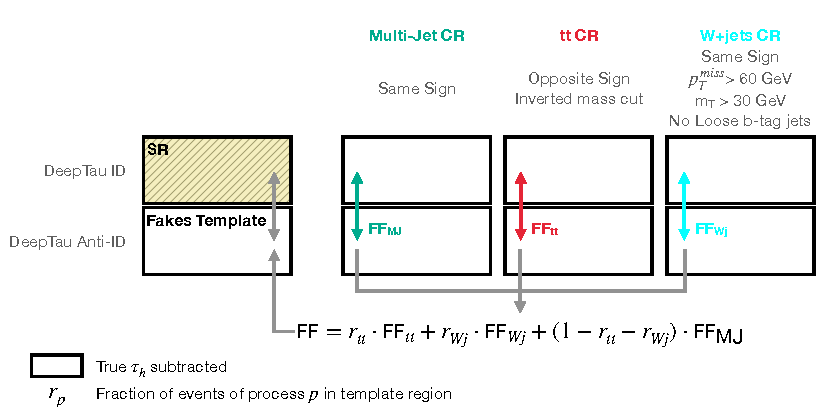
\includegraphics[width=\linewidth, trim=4bp 0bp 0bp 13bp, clip]{figures/chapter_V/ff_regions.pdf}
    \caption[Regions used in the Fake Factor method]{%
        Schematic representation of the regions used to estimate the
        contribution of fakes based on the data. Each region is divided into two halves depending on whether the $\tau_h$ candidate passes (top) or fails (bottom) the Medium WP of the discriminant against jets. In the sideband regions, the ratio between the two halves defines the fake factor of each process; the lower half of the signal region is the
        template region, to which they are applied.}
    \label{fig:ff_regions}
\end{figure}


\subsection{Validation of the method} 
%
The fake factors of each process are measured in a region dominated by that process, but their application to the signal regions relies on their being transferable to events not used in their derivation. For the QCD multi-jet component, this is tested directly in a dedicated validation region, orthogonal to all the previous ones, in which the two $\tau_h$ candidates have the same charge and the two jets of the $H\to b\bar{b}$ candidate fail the Medium working point of the $b$ tagging discriminant, with only one of them passing the Loose one. These requirements suppress the processes with genuine $\tau\tau$ pairs, $t\bar{t}$, and $W$+jets, so that $99\%$ of the events contain a misidentified jet that originates almost entirely from QCD multi-jet production, and the multi-jet fake factor is therefore applied alone. It is applied to the events whose second $\tau_h$ fails the Medium working point, and the resulting prediction is compared with the events in which it passes. Since the fake factor is derived in a different region, the agreement is not guaranteed by construction. as a function of the $p_T$ of the second $\tau_h$, one of the variables in which the fake factor is parameterized, and of the reconstructed mass of the $HH$ system, which does not enter its parameterization but is one of the main observables of the signal extraction. In both, the prediction reproduces the data within the statistical uncertainties over the whole range. The $t\bar{t}$ and $W$+jets fake factors are instead tested through the agreement of the complete prediction in the categories of the analysis, examined in Section \ref{sec:bbtt_controlplots}.
%
\begin{figure}[tbp]
    \centering
    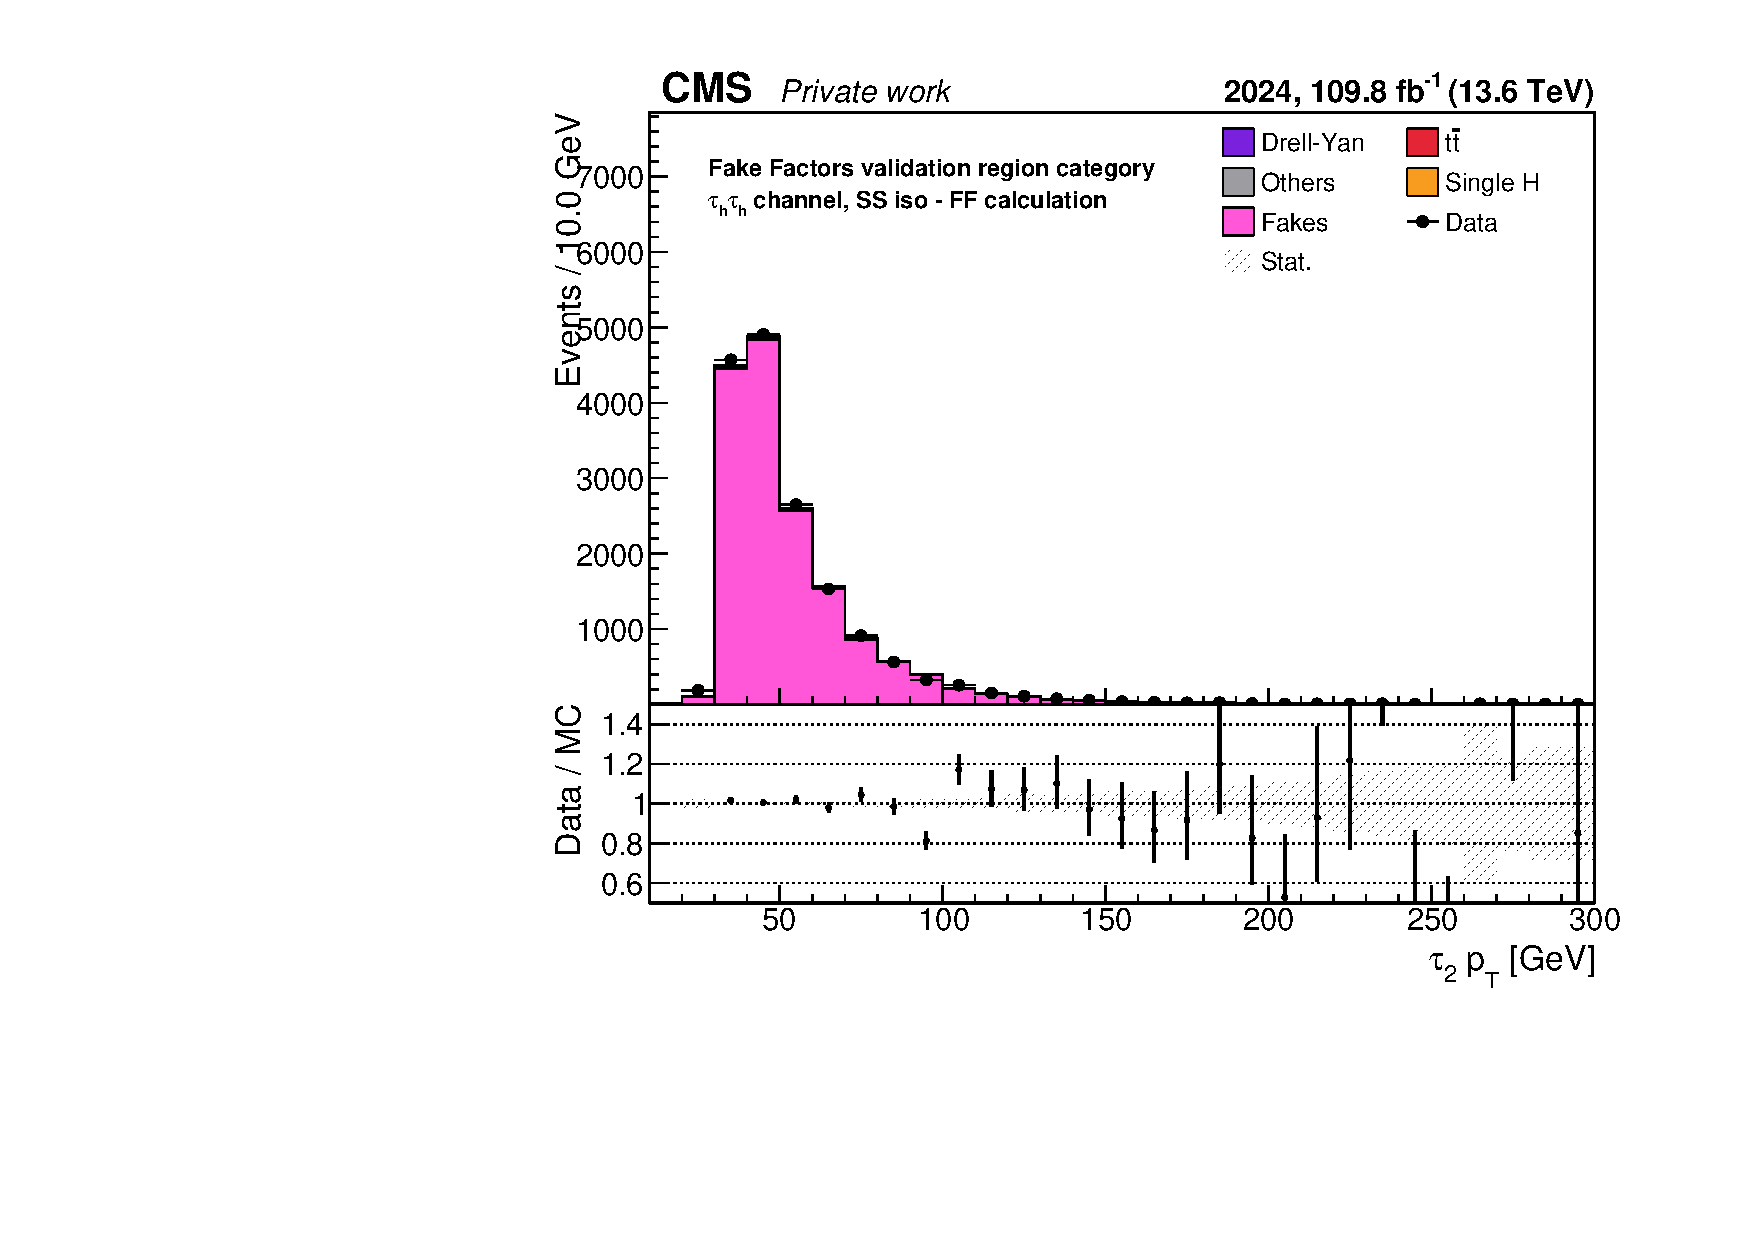
\includegraphics[width=0.49\linewidth, trim=11bp 0bp 40bp 14bp, clip]{figures/chapter_V/lep2_pt__tautau_ss_isoFFcalc__pg_forPlots__ff__stack.pdf}
    \hfill
    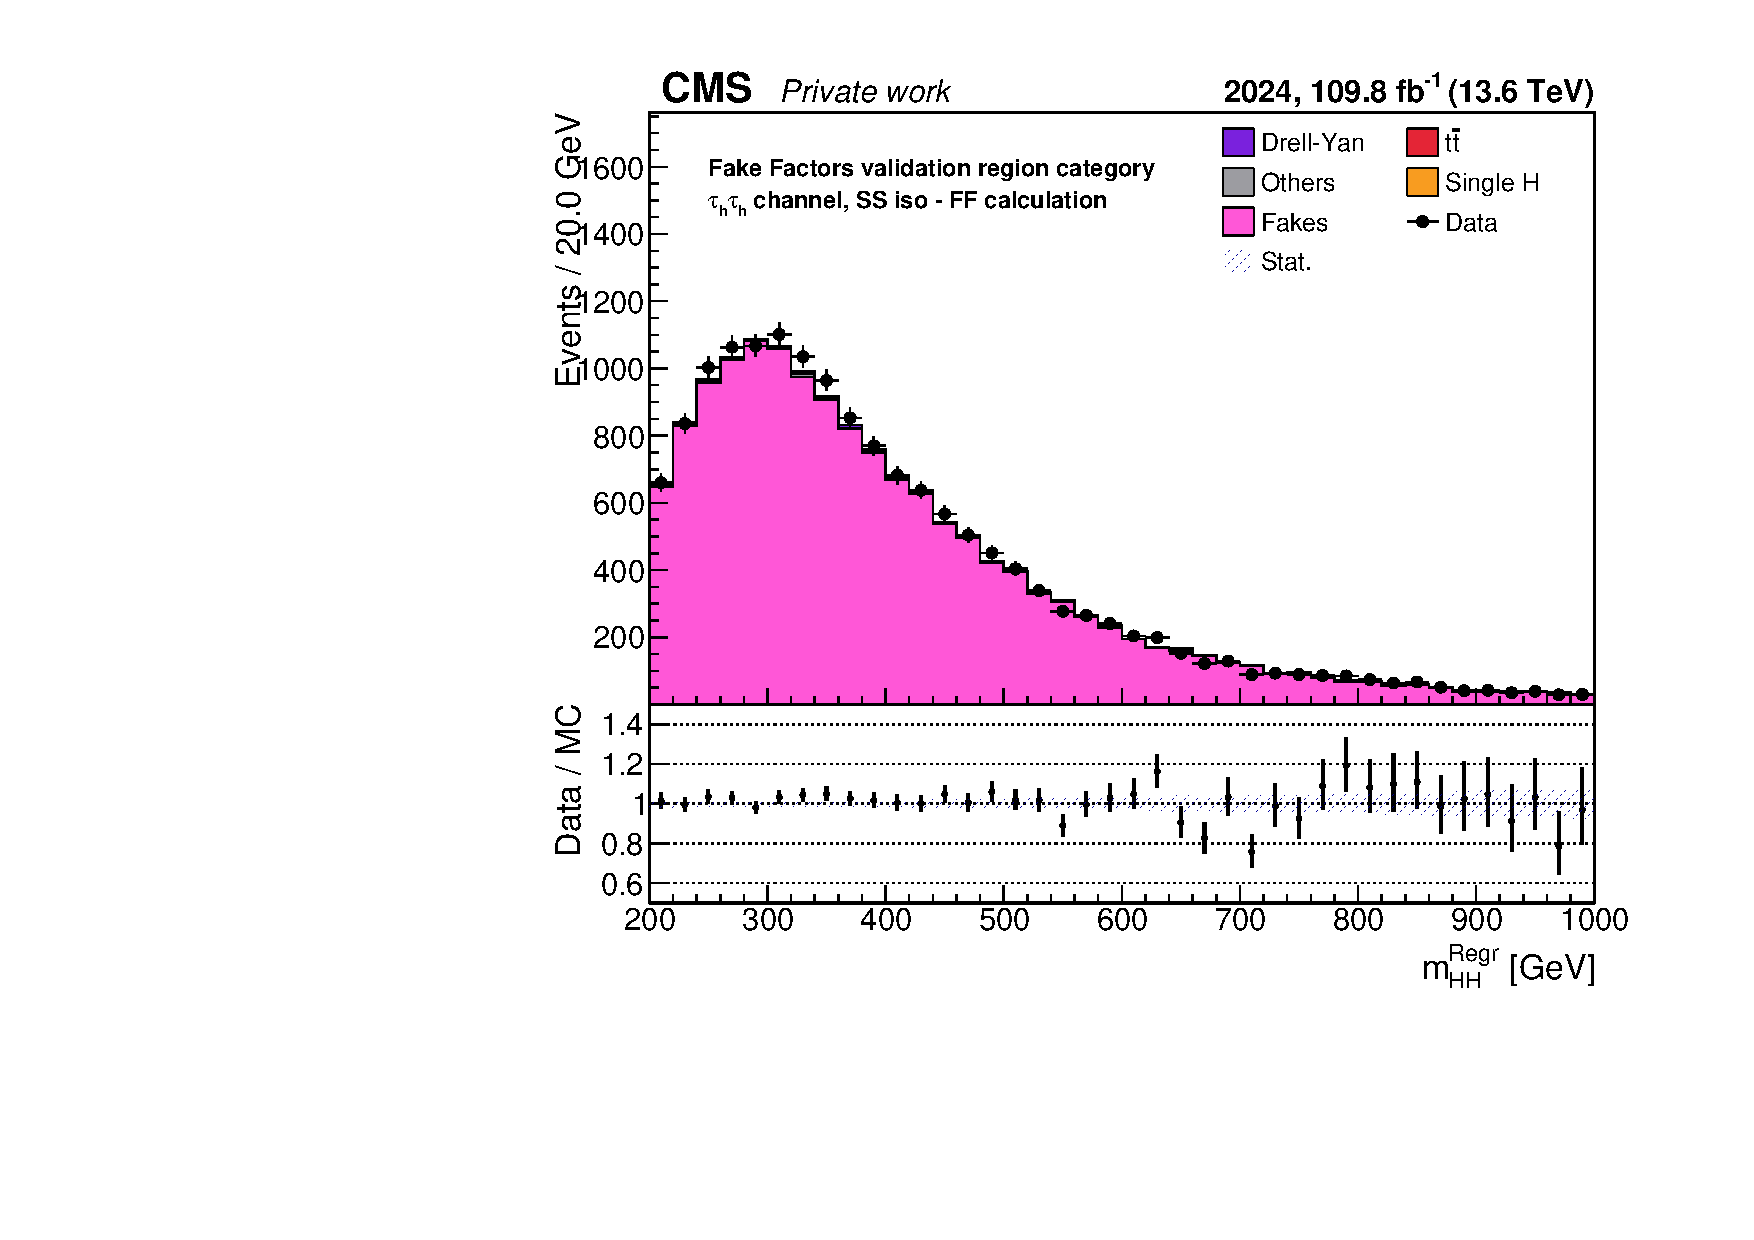
\includegraphics[width=0.49\linewidth, trim=11bp 0bp 40bp 14bp, clip]{figures/chapter_V/HH_regr_mass_thesis__tautau_ss_isoFFcalc__pg_forPlots__ff__stack.pdf}
    \caption[Closure of the fake factor method]{%
        Distributions of the $p_T$ of the second $\tau_h$ candidate (left) and of the
        reconstructed mass of the $HH$ system (right) in the validation region of the fake
        factor method, for the $\tau_h\tau_h$ channel in 2024. The prediction of misidentified
        jets is obtained by applying the multi-jet fake factor to the events in which the
        second candidate fails the Medium working point, and the band shows its statistical
        uncertainty.}
    \label{fig:ff_closure}
\end{figure}




\bigskip


The prediction of the background in each signal region has been described. While processes with genuine $\tau_h$ candidates are taken from the simulation, corrected as described in Section \ref{sec:bbtt_corrections}, the contribution of fakes is estimated directly from the data. Each of these components carries its own uncertainties, including, for the fake factor estimate, those arising from the statistics of the regions used and those propagated from the calibration of the objects that define them. These uncertainties are described in the next section.



\section{Systematic uncertainties}
\label{sec:bbtt_systematics}
%
Each element of the prediction described in the previous sections carries an uncertainty, and the resulting sources of uncertainty fall into three families. Theoretical uncertainties reflect the limited knowledge of the cross sections and branching fractions used to normalize the simulated samples, as well as the effect of the same variations on the fraction of selected events. Experimental uncertainties stem from the integrated luminosity and from the limited precision of the corrections in Section \ref{sec:bbtt_corrections}, which also affect the estimate of misidentified jets in Section \ref{sec:bbtt_ff} through the objects that define the sideband and template regions in which it is measured and applied. Statistical uncertainties, finally, reflect the finite number of events, both in the simulated samples and in the sideband and template regions used for that estimate.

The following subsections review these sources grouped by the part of the prediction they affect. All of them are incorporated into the statistical model as nuisance parameters, which modify either only the normalization of the affected process or also the shape of its distributions, as described in Section \ref{subsec:bbtt_nuisances}, and their impact on the result is discussed in Section \ref{sec:bbtt_results}.

\subsection{Luminosity and theoretical uncertainties}
%
The number of events that each simulated process contributes to the prediction is the product of the integrated luminosity, the production cross section, the branching fractions of the Higgs bosons involved, and the acceptance, defined as the fraction of generated events that pass the selection. The first three factors scale the yield of the process without altering the shape of its distributions, whereas the acceptance depends on the kinematics of the events and can modify it. Therefore, these factors correspond to sources of uncertainty independent of the correction applied to the simulation, and they affect all processes derived from the simulation.

\subsubsection{Integrated luminosity} 
%
The integrated luminosity for each year is derived from van der Meer scans and the stability of the response of the detectors used to monitor it, and is known with a precision of $1.4\%$ in 2022 \cite{CMS-PAS-LUM-22-001}, $1.3\%$ in 2023~\cite{CMS-DP-2024-068}, and $1.7\%$ in 2024~\cite{CMS-DP-2026-003}, partially correlated between years through their common sources. Because luminosity is the factor by which all simulated samples are normalized, this uncertainty applies to the signal and to all simulated backgrounds, but not to the estimate of misidentified jets, which is obtained directly from the data.

\subsubsection{Cross sections and branching fractions} 
%
The cross sections used to normalize the simulated samples are fixed-order calculations, and their uncertainty is evaluated by varying the different inputs to the calculation: the renormalization and factorization scales, the set of parton distributions, and the value of $\alpha_s$. For $HH$ production via gluon fusion, the uncertainty in the cross section from the scale variation, combined with the ambiguity in the top quark mass scheme, amounts to $^{+6}_{-23}\%$~\cite{Grazzini:2018bsd,Baglio:2020wgt}, and that from the parton distributions and $\alpha_s$ to $2.3\%$, while for vector boson fusion the same sources change the cross section by $0.05\%$ and $2.7\%$, respectively~\cite{Dreyer:2018qbw,Dreyer:2020xaj}. Since the scale variation depends on $\kappa_\lambda$, it is reevaluated for each coupling hypothesis.


For the simulated backgrounds, the recommended uncertainties of each process are used, ranging from $0.5$ to $6\%$\cite{LHCHWG-xsec-13p6TeV}, with two exceptions: Drell--Yan is normalized with the correction derived from data in Section \ref{sec:bbtt_corrections} rather than with its theoretical cross section; and the production of a Higgs boson in association with a $b\bar{b}$ pair, which enters precisely the $b$-tagged categories in which the signal is searched for, and whose predicted rate there is considerably less well known than that of the other single Higgs processes\cite{bbH-modelling}, is assigned an additional $100\%$ normalization uncertainty.

%whose predicted rate is affected by a large theoretical uncertainty arising from the treatment of the $b$-quark parton density and from the choice of flavor scheme in the calculation \cite{bbH-modelling}.


Finally, the $H\to b\bar{b}$ and $H\to\tau\tau$ decay branching fractions are known with a precision of $^{+1.2}_{-1.3}\%$ and $^{+1.7}_ {-1.6}\%$ \cite{deFlorian:2016spz}, and their uncertainty is assigned to all processes, including the signal, involving at least one Higgs boson.


\subsubsection{Effects on the acceptance} 
%
The theoretical variations above do not only change the inclusive cross section. By altering the momentum distribution of the initial partons and the probability of emitting additional radiation, they also change the kinematics of the events and therefore the fraction that passes the selection, an effect that is evaluated separately. To the renormalization and factorization scales and the parton distributions, a third variation is added here, that of the parameters of the parton shower, which does not change the total cross section but modifies the number and hardness of the additional jets, and with them the category into which each event is ultimately classified. For each process and category, the acceptance under each variation is recomputed as the ratio of selected to generated events, so that the change in the inclusive cross section cancels in the ratio and is not counted twice.

This yields three acceptance uncertainties — one per type of variation — which are evaluated in each bin of the fitted distribution, so that they can modify its shape and not only the yield of the category. Among them, the parton shower variation has the largest effect on the acceptance, typically $4\%$ and up to $9\%$, followed by the scale variation, about $2\%$, while the parton distribution variation changes it by less than $1\%$, although all three are included in the fit. They are evaluated for the signal and for the main simulated backgrounds, Drell--Yan, $t\bar{t}$, and single Higgs production, whereas for the remaining simulated backgrounds, which contribute little to the categories, they are not considered, since their effect is negligible compared with the normalization uncertainty already assigned to these processes.\medskip


%que modifica la distribución de cada proceso, y que son las escalas de renormalización y factorización y las distribuciones de partones que ya aparecían como fuente de incertidumbre para la sección eficaz inclusiva, con el añadido de los parámetros de la lluvia de partones. Éstas se asignan a los procesos que contribuyen en cada categoría, y se evalúan intervalo a intervalo. Las asociadas a las distribuciones de partones resultan ser despreciables y las de las escalas se mantienen en torno al 1\%, mientras que las de la lluvia de partones son las mayores de las tres.\\



%sin repetir la reconstrucción, ya que ninguna de las tres altera la energía ni la dirección de los objetos reconstruidos.


\subsection{Uncertainties in the object-level corrections}
%
The object-level corrections of Section \ref{subsec:bbtt_object_corrections} apply to all simulated processes, including the signal. Most come from the central CMS recommendations together with their uncertainties, while those derived within the analysis carry an uncertainty estimated with the measurement itself. In particular, the $15\%$ non-closure of the factorized QuadJet trigger efficiency (Figure \ref{fig:quadjet_closure}) is added to the uncertainty of its measurement; the identification factors of the $b\tau_h\tau_h$ candidates also carry their own uncertainty; and so do the two components of the $b$ tagging calibration derived internally, namely the tagging efficiencies measured in simulation — used in 2024 to turn the \textsc{UParT} working point scale factors into a per-event weight —, and the dedicated calibration of large-radius jets misidentified as $H\to b\bar{b}$ candidates.\medskip

For each source, two alternative distributions are built in addition to the nominal one by shifting the correction by one standard deviation up and down. When the correction is a weight — trigger, reconstruction, identification, isolation, and tagging scale factors — the histograms are refilled with the shifted weight. When it modifies the energy of the objects — the energy scales and resolutions of jets, electrons, and $\tau_h$ — events can migrate between categories and the inputs of the final discriminant change, so the full analysis chain is repeated with the shifted correction, which is also propagated consistently to $p_T^\text{miss}$. None of these corrections is the same for all events, so in both cases the variation changes both the normalization and the shape of the distributions. Table \ref{tab:object_systematics} lists these sources in the order in which the corrections were presented, providing a detailed breakdown of each uncertainty, indicating its origin and the method employed to propagate it.
% The pile-up reweighting is the one exception, as the shape information of its variation is removed for the background processes before the fit, in the way described in Section \ref{sec:bbtt_statistics}.
\begin{table}[tbp]
\centering
\small
\setlength{\tabcolsep}{4pt}
\begin{tabular}{@{}l>{\raggedright\arraybackslash\hyphenpenalty=10000\exhyphenpenalty=10000}p{3.6cm}llr@{}}
\toprule
Correction & Components & Source & Propagated as & Effect \\
\midrule
Pile-up reweighting\tablefootnote{Evaluated by varying by $4.6\%$~\cite{CMS-inelastic-13TeV} the inelastic proton-proton cross section, from which the pile-up profile in data is inferred, and reweighting the simulation to each of the two shifted profiles.}
                                     & 1                                     & central & event weight        & $0.7$--$6\%$ \\
Trigger efficiency                   & one per separately measured component & both    & event weight        & $0.3$--$8\%$ \\
Muon identification and isolation    & 2                                     & central & event weight        & $0.1$--$0.2\%$ \\
Electron reconstruction              & 2, split at $p_T = 20$ GeV            & central & event weight        & $0.2$--$0.8\%$ \\
Electron identification              & 1                                     & central & event weight        & $0.4$--$1.2\%$ \\
Electron energy scale and resolution & 2                                     & central & object energy shift & ${<}\,1\%$ \\
$\tau_h$ identification              & against jets, electrons,\newline and muons    & both    & event weight        & ${<}\,3\%$ \\
$\tau_h$ energy scale                & period dependent                      & central & object energy shift & $0.2$--$1.3\%$ \\
Jet energy scale                     & several, one per calibration step     & central & object energy shift & $0.7$--$6\%$ \\
Jet energy resolution                & 1                                     & central & object energy shift & $0.3$--$6\%$ \\
$b$ tagging of small-radius jets     & algorithm and period dependent        & both    & event weight        & $1$--$7\%$ \\
Tagging of the large-radius jet      & 2                                     & both    & event weight        & $2$--$17\%$ \\
\bottomrule
\end{tabular}
\caption[Uncertainties in the object-level corrections]{%
    Sources of uncertainty associated with the object-level corrections described in
    Section \ref{subsec:bbtt_object_corrections}. The last column gives the typical effect of
    each correction on the expected yield of the main processes: for each process and category,
    its components and data-taking periods are combined in quadrature, and the range between
    the 10th and 90th percentiles of the resulting values across processes and categories is
    quoted.}
\label{tab:object_systematics}
\end{table}
% 1) se parte de las diez datacards de HIG-25-008 (una por cada categoria y canal); cada una contienen para cada proceso el histograma nominal de la salida de la DNN, y para cada fuente, sus histogramas up y down (prediccion con esa fuente desplazada +-1sigma); 
% 2) para acada combinacion se suman los bins de cada histograma, lo que da el numero total de sucesos esperados, y se calcula cuanto cambia respecto al nominal (para las fuentes lnN el efecto se lee directamente de la datacard)
%3) solo para los procesos principales (DY, tt, signal HH ggHH y qqHH, fakes)
% 4) se juntan las componentes de cada fila de la tabla: combinadas en cuadratura para cada proceso y categoria (porque son nuisance parameters independientes) - incluye las componentes de la correccion como su division por periodos
% 5) 10 categorias x 4 procesos simulados: se toman los percentiles 10 y 90



%\paragraph{Pile-up reweighting} A diferencia del perfil de la simulación, que se fija de antemano, la distribución del número de interacciones en los datos se infiere a partir de la luminosidad instantánea de cada cruce de haces y de la sección eficaz inelástica protón-protón. La incertidumbre de la reponderación está dominada por la de esta última, y se evalúa variando su valor en un $4.6\%$, de acuerdo con su medida a $13$ TeV \cite{CMS-inelastic-13TeV}, y recalculando los pesos de la simulación con cada una de las dos distribuciones resultantes. 



% La correlación de cada fuente entre periodos de toma de datos sigue las recomendaciones de los grupos responsables de cada objeto o, en el caso de las calibraciones derivadas en el propio análisis, el modo en que se han medido.\\



%\paragraph{Pile-up reweighting} A diferencia del perfil de la simulación, que se fija de antemano, la distribución del número de interacciones en los datos se infiere a partir de la luminosidad instantánea de cada cruce de haces y de la sección eficaz inelástica protón-protón. La incertidumbre de la reponderación está dominada por la de esta última, y se evalúa variando su valor en un $4.6\%$, de acuerdo con su medida a $13$ TeV \cite{CMS-inelastic-13TeV}, y recalculando los pesos de la simulación con cada una de las dos distribuciones resultantes. 



%Los pesos se calculan por separado para cada uno de los cinco periodos, pero la variación de la sección eficaz es común a todos ellos, de modo que en el ajuste la incertiumbre asociada se trata como una única fuente, correlacionada entre periodos.


%\paragraph{Trigger efficiency scale factors} Los factores de escala de disparo llevan una incertidumbre por cada una de las componentes que se miden por separado. 
%Todas ellas se tratan como independientes entre periodos, puesto que cada factor se mide por separado en cada uno. 
%En el caso del camino QuadJet de 2024, a la incertidumbre de la propia medida se añade la falta de cierre del $15\%$ observada en la validación de la factorización. \textcolor{red}{[CONFIRMAR ESTO]}


%\paragraph{Muons and electrons} Las incertidumbres de los factores de escala de muones y electrones se toman de las medidas centrales de los grupos de CMS responsables de cada objeto, proporcionadas junto con los propios factores. Para los muones se consideran las de identificación y de aislamiento, y para los electrones, las de identificación, que incluye el aislamiento, y las de reconstrucción. Estas últimas se proporcionan por separado por debajo y por encima de 20 GeV, ya que se derivan con técnicas distintas, y sus incertidumbres se tratan como independientes. Todas estas incertidumbres se propagan como pesos. En el caso de los electrones se añaden, además, las incertidumbres en la escala y la resolución de su energía, que se propagan desplazando la energía de los electrones simulados y repitiendo la cadena de análisis.




%\paragraph{Hadronic \texorpdfstring{$\tau$}{tau} leptons} Tanto los factores de escala de identificación de los $\tau_h$ como la corrección de su escala de energía se toman, junto con sus incertidumbres, de las recomendaciones centrales de CMS. Por un lado, los factores de identificación frente a jets, electrones y muones se propagan como pesos. Por otro, la escala de energía \cite{CMS-TAU-24-001} se propaga desplazando la energía de los $\tau_h$ simulados. La excepción son los candidatos del canal $b\tau_h\tau_h$, cuyos factores de identificación se miden dentro del propio análisis y llevan una incertidumbre independiente.


%\paragraph{Jets and \texorpdfstring{$p_T^\text{miss}$}{pTmiss}} Las incertidumbres en la escala de energía de los jets y en la corrección de su resolución se toman igualmente de las recomendaciones centrales de CMS. Las primeras se descomponen en varias fuentes asociadas a los distintos pasos de la calibración, y la segunda constituye una fuente adicional. Ambas se propagan desplazando la energía de todos los jets simulados y a través de ellos a $p_T^\text{miss}$. \textcolor{red}{confirmar si es verdad que se descomponen en varias fuentes} 


%\paragraph{Identification of \texorpdfstring{$b$}{b} jets} Las incertidumbres de los factores de escala del etiquetado de jets de $b$, tanto para los jets de radio pequeño como para el candidato de radio grande de la categoría \textit{boosted}, se toman de las recomendaciones centrales de CMS para el algoritmo y el método de calibración empleados en cada periodo, descritos en la Sección \ref{subsec:bbtt_object_corrections}, y se propagan como pesos. La excepción son las dos componentes de la calibración derivadas dentro del propio análisis, que llevan incertidumbres propias: las eficiencias de etiquetado medidas en la simulación, necesarias en 2024 para aplicar los factores de escala de \textsc{UParT} por puntos de trabajo, y la calibración dedicada de los jets de radio grande mal identificados como candidatos $H\to b\bar{b}$.


\subsection{Uncertainties in the process-specific corrections}
%
The uncertainties associated with the corrections to the two dominant backgrounds in Section \ref{subsec:bbtt_process_corrections} are evaluated within the analysis itself, since neither stems from a central recommendation, and both are propagated as weights.

The Drell--Yan correction is the product of two factors, each of which contributes its own sources of uncertainty. The first factor, the fit of the ratio between data and simulation as a function of the $p_T$ of the muon pair, uses a function that is Gaussian at low $p_T$ and linear at high $p_T$, and the boundary between the two regimes, $p_T^0$, is itself a parameter of the fit. Rather than varying each fit parameter, one source is defined per regime, and the value of $p_T^0$ from the nominal fit determines which bins belong to each. For the Gaussian regime, the content of the bins below $p_T^0$ is shifted upward by $1.5$ times its statistical uncertainty while the bins above are left unchanged, and the refit yields the upward variation of the correction. Shifting the same bins downward yields the downward variation. The source of the linear regime is built in the same way from the bins above $p_T^0$. The second factor, the normalization in bins of $n_\text{jets}$ and $n_{b\,\text{jets}}$, carries the statistical uncertainty of its measurement, grouped into three sources, one per bin of $n_{b\,\text{jets}}$, within which the five bins of $n_\text{jets}$ shift simultaneously. Together, these sources change the Drell--Yan yield by about $1\%$, and at most by $2\%$, across the categories.

The correction to the top quark $p_T$, being a calculation rather than a measurement, has no independent estimate of its accuracy, and is therefore assigned an uncertainty equal to the correction itself, applying it twice for the upward variation and not applying it for the downward one, so that the nominal value lies midway between the two. It affects only the $t\bar{t}$ samples, since single top quark production does not carry the correction, and its effect on the $t\bar{t}$ yield is typically $1$--$2\%$, and reaches $6\%$ in the categories where the top quarks are most energetic.

\subsection{Uncertainties in the jet\texorpdfstring{$\to\tau_h$}{ -> tau h} estimate}
%
Since the estimate of Section \ref{sec:bbtt_ff} does not come from the simulation, none of the above uncertainties apply to it directly. Its uncertainties come instead from the calibration of the objects that define its regions — which enters the measured factors — and from the finite number of events in the regions where the method is measured and applied.

To quantify the first, the fake factors are derived again under the same energy scale and resolution shifts of $\tau_h$, electrons, and jets listed in Table \ref{tab:object_systematics}. The effect is found to be smaller than the statistical uncertainty of the method except for the $t\bar{t}$ component, so a single source is defined as an envelope for each process that grows linearly with the $p_T$ of the candidate, from $20\%$ at $20$ GeV to $100\%$ at $200$ GeV for $t\bar{t}$, and from $1\%$ to $5\%$ for $W$+jets and QCD multi-jet, with the three shifting together. A second source is the statistical uncertainty of the three fake factors, $FF_\text{MJ}$, $FF_{t\bar{t}}$, and $FF_{Wj}$ — measured in the auxiliary regions — and of the fractions $r_{t\bar{t}}$ and $r_{Wj}$ with which they are combined in Equation \ref{eq:fake_factor}, propagated by shifting them consistently. Both are propagated as weights on the events of the template region. The envelope changes the yield of misidentified jets by about $20\%$, and the statistical uncertainty of the fake factors and fractions by about $10\%$.

The third source is the number of events in the template region itself, which often amounts to a few events per bin, or none. In this regime the Gaussian approximation does not describe the Poisson distribution, and an empty bin would carry no uncertainty. The count of the template in each bin is therefore assigned the Garwood interval~\cite{Garwood:1936} at $95\%$ confidence level\footnote{A $95\%$ confidence interval overestimates the statistical uncertainty of the template region by approximately a factor of two. This choice is deliberately conservative, as this is the first application of this method in the search.}, which respects the asymmetry of the Poisson distribution and is also defined for zero counts. This interval is converted into an uncertainty on the prediction by multiplying it by the average fake factor of the bin or, for empty bins, by the largest average fake factor among the non-empty ones. Unlike the other two, this source is built directly on the final distribution, bin by bin. This source also amounts to about $10\%$ of the yield of misidentified jets, and reaches $15\%$ in the least populated categories.



\subsection{Statistical uncertainties of the simulated samples}
%
Each simulated process is built from a finite number of generated events, so the content of each bin of the fitted distribution is subject to statistical fluctuation. Following the method of Barlow and Beeston~\cite{Barlow:1993dm}, the prediction in each bin is allowed to vary within its statistical uncertainty, constrained by a term that reflects the number of simulated events behind it, which adds one parameter per bin to the fit.

The samples used for each process are listed in Table \ref{tab:mc_backgrounds}. For the dominant backgrounds, $t\bar{t}$ and Drell--Yan, the samples are large enough for this uncertainty to remain small, as shown in Table \ref{tab:mc_stats_2024} for 2024, where the equivalent integrated luminosity of each sample, $\mathcal{L}_\text{eq} = N_\text{gen}/\sigma$, exceeds the $109.8$ fb$^{-1}$ recorded in that year by a factor between about $3$ and $40$.\bigskip
\begin{table}[tbp]
\centering
\small
\begin{tabular}{@{}llrrr@{}}
\toprule
Process & Sample & $\sigma\cdot\mathcal{B}$ [pb] & $N_\text{gen}$ [$10^6$] & $\mathcal{L}_\text{eq}$ [fb$^{-1}$] \\
\midrule
$t\bar{t}$ & dileptonic   & $98.0$  & $470.1$ & $4795$ \\
           & semileptonic & $405.7$ & $484.5$ & $1194$ \\
           & hadronic     & $419.7$ & $472.5$ & $1126$ \\
\midrule
$Z/\gamma^{*}\to\tau\tau$ + jets & 0 jets & $1684.0$ & $493.1$ & $293$ \\
                                 & 1 jet  & $318.5$  & $428.4$ & $1345$ \\
                                 & 2 jets & $120.7$  & $233.0$ & $1930$ \\
\bottomrule
\end{tabular}
\caption[Size of the main simulated background samples in 2024]{Number of generated events and equivalent integrated luminosity, $\mathcal{L}_\text{eq} = N_\text{gen}/\sigma$, of the main simulated background samples in 2024, to be compared with the $109.8$ fb$^{-1}$ of data recorded in that year.}
\label{tab:mc_stats_2024}
\end{table}
% Esta tabla me da la luminosidad equivalente que me dice cuantos datos habria que tomar para tener de ese procesos tantos sucesos como la muestra simulada. Es decir, si ttdileptonic tiene 470 milones de sucesos y sec de 98pb, para que el LHC produjera esos sucesos haria falta lumi de 4795, es decir, 44 veces mas que los datos de 2024. Esto importa portque para normalizar la simulacion a los datos, cada suceso simulado se pesa con 
% w = sigma * Ldatos/Ngen, es decir: L datos / Leq = 1/44; fluctuacion estadistica relativa del MC es sqrt44 veces menor que la de los datos; si el factor fuera menor que 1 (como podria ser para los wjets con 1 jet y bajo pt) cada sucesos simulado pesa mas que uno real y la simulacion fluctua mas que los datos en esa zona - todo esto aproximado (no tiene encuenta pesos negativos de muestras NLO)


   


With these sources, the prediction is complete. The correlation assigned to each of them across categories and data-taking periods is described in Section \ref{subsec:bbtt_nuisances}, and their weight on the measurement, which can only be determined after the fit, in Section \ref{sec:bbtt_results}. Before that, Section \ref{sec:bbtt_controlplots} compares the prediction with the data, with an uncertainty band that combines all the sources just described, to check whether the corrections and the estimate of misidentified jets reproduce the observations within the margin assigned to them.
    


\section{Pre-fit distributions}
\label{sec:bbtt_controlplots}
%
Section \ref{sec:bbtt_flow} defines the ten categories into which the dataset for each period is divided, as shown in Figure \ref{fig:categories}. The corrections and methods derived within the analysis itself have already been validated  in the respective derivation and validation regions. It remains to be verified that the complete prediction — with all corrections applied simultaneously and using the full selection from the analysis — accurately describes the observed data. Its normalizations and shapes are those that result directly from the corrected simulation and from the fake factors method, without any fitted to the data. This is therefore the only comparison in which a discrepancy indicates a problem in the modeling rather than an artifact of the fit.

The comparison is presented in two steps. First, it shows the agreement in control regions dominated by only one of the main backgrounds, where the contribution of the signal is negligible and the agreement can be unambiguously attributed to the process being validated. Second, it examines the categories of the analysis themselves, where the background is a mixture of all processes and where the goal is to verify that the complete prediction reproduces the data.



\subsection{Control regions}
\label{subsec:bbtt_cr}
%
The two regions studied here are enriched in the two dominant backgrounds, Drell--Yan and $t\bar{t}$ production, both are taken from the simulation with their specific corrections. The remaining simulated processes carry only the common corrections, and their combined contribution, grouped under \textit{Others} in the figures, is small.\medskip

Both regions are built from the categories of Section \ref{sec:bbtt_flow}, with the same selection and corrections, in the control channels with two light leptons of opposite charge reserved in the channel assignment. They are therefore orthogonal to the signal regions through their lepton content, and otherwise share their phase space, so that the corrections are tested in an environment kinematically close to the one in which they are applied, but free of signal.\medskip

The Drell--Yan-enriched region is the res1b category in the $ee$ channel, with a dilepton mass between $70$ and $110$ GeV, in order to isolate the $Z$ boson peak, and $p_T^\text{miss} < 45$ GeV to suppress processes with neutrinos in the final state, mainly $t\bar{t}$. In this control region, Drell--Yan production accounts for about 96$\%$ of the prediction. Its kinematic selection is the one used to derive the Drell--Yan correction in Section \ref{sec:bbtt_corrections}, with two differences that make the test independent. The correction was measured in the $\mu\mu$ channel, and the multiplicity of $b$-tagged jets entered it as a binning variable, whereas here the $b$ tagging requirement of the res1b category is part of the selection.

The $t\bar{t}$-enriched region is the res2b category in the $e\mu$ channel, where the two genuine $b$ jets and the $e\mu$ pair, which suppresses Drell--Yan, yield a $t\bar{t}$ purity of about 96$\%$.\medskip

Figures \ref{fig:cr_dy} and \ref{fig:cr_tt} compare the data and the prediction in the two regions for 2024. In the Drell--Yan region, the $p_T$ of the lepton pair and the number of jets are the variables on which the correction acts, while the masses of the $H\to b\bar{b}$ candidate and of the $HH$ system were not used in its derivation but enter the signal extraction. In the $t\bar{t}$ region, the $p_T$ of the leading $b$ jet is sensitive to the correction of the top quark $p_T$, and $p_T^\text{miss}$ to the two neutrinos of the dileptonic decay. The prediction describes the data within the uncertainties in both regions, with total yields that agree to within $3\%$. The only visible deviation appears in the tail of $m_{HH}$ in the Drell--Yan region, where the data exceed the prediction by $10$ to $30\%$ above about $600$ GeV.
%
\begin{figure}[tbp]
    \centering
    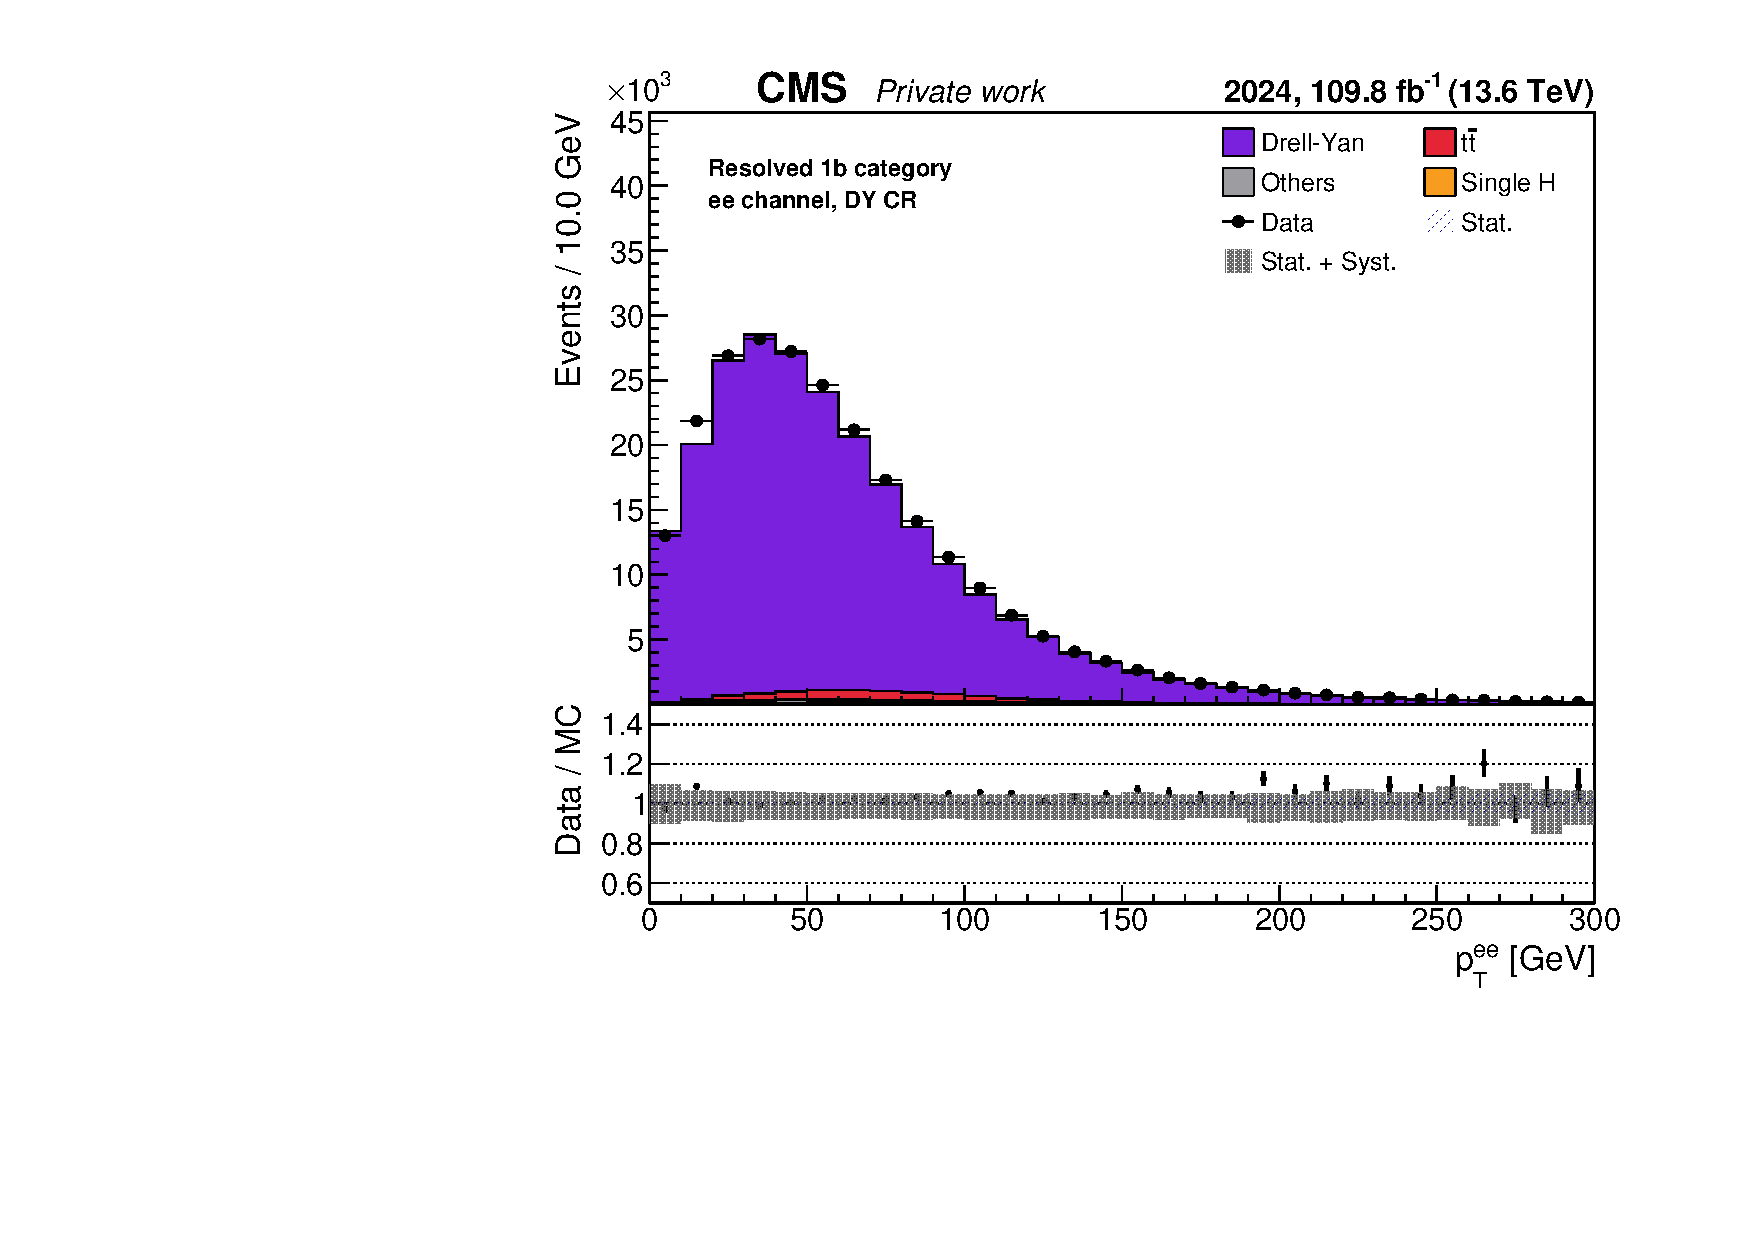
\includegraphics[width=0.49\linewidth, trim=11bp 0bp 40bp 14bp, clip]{figures/chapter_V/CR_res1b/THESIS_CR_DYCR_Prod_26_04_thesis/Htt_pt__ee_os_iso_DYCR__pg_forPlotsCR__stack.pdf}\hfill
    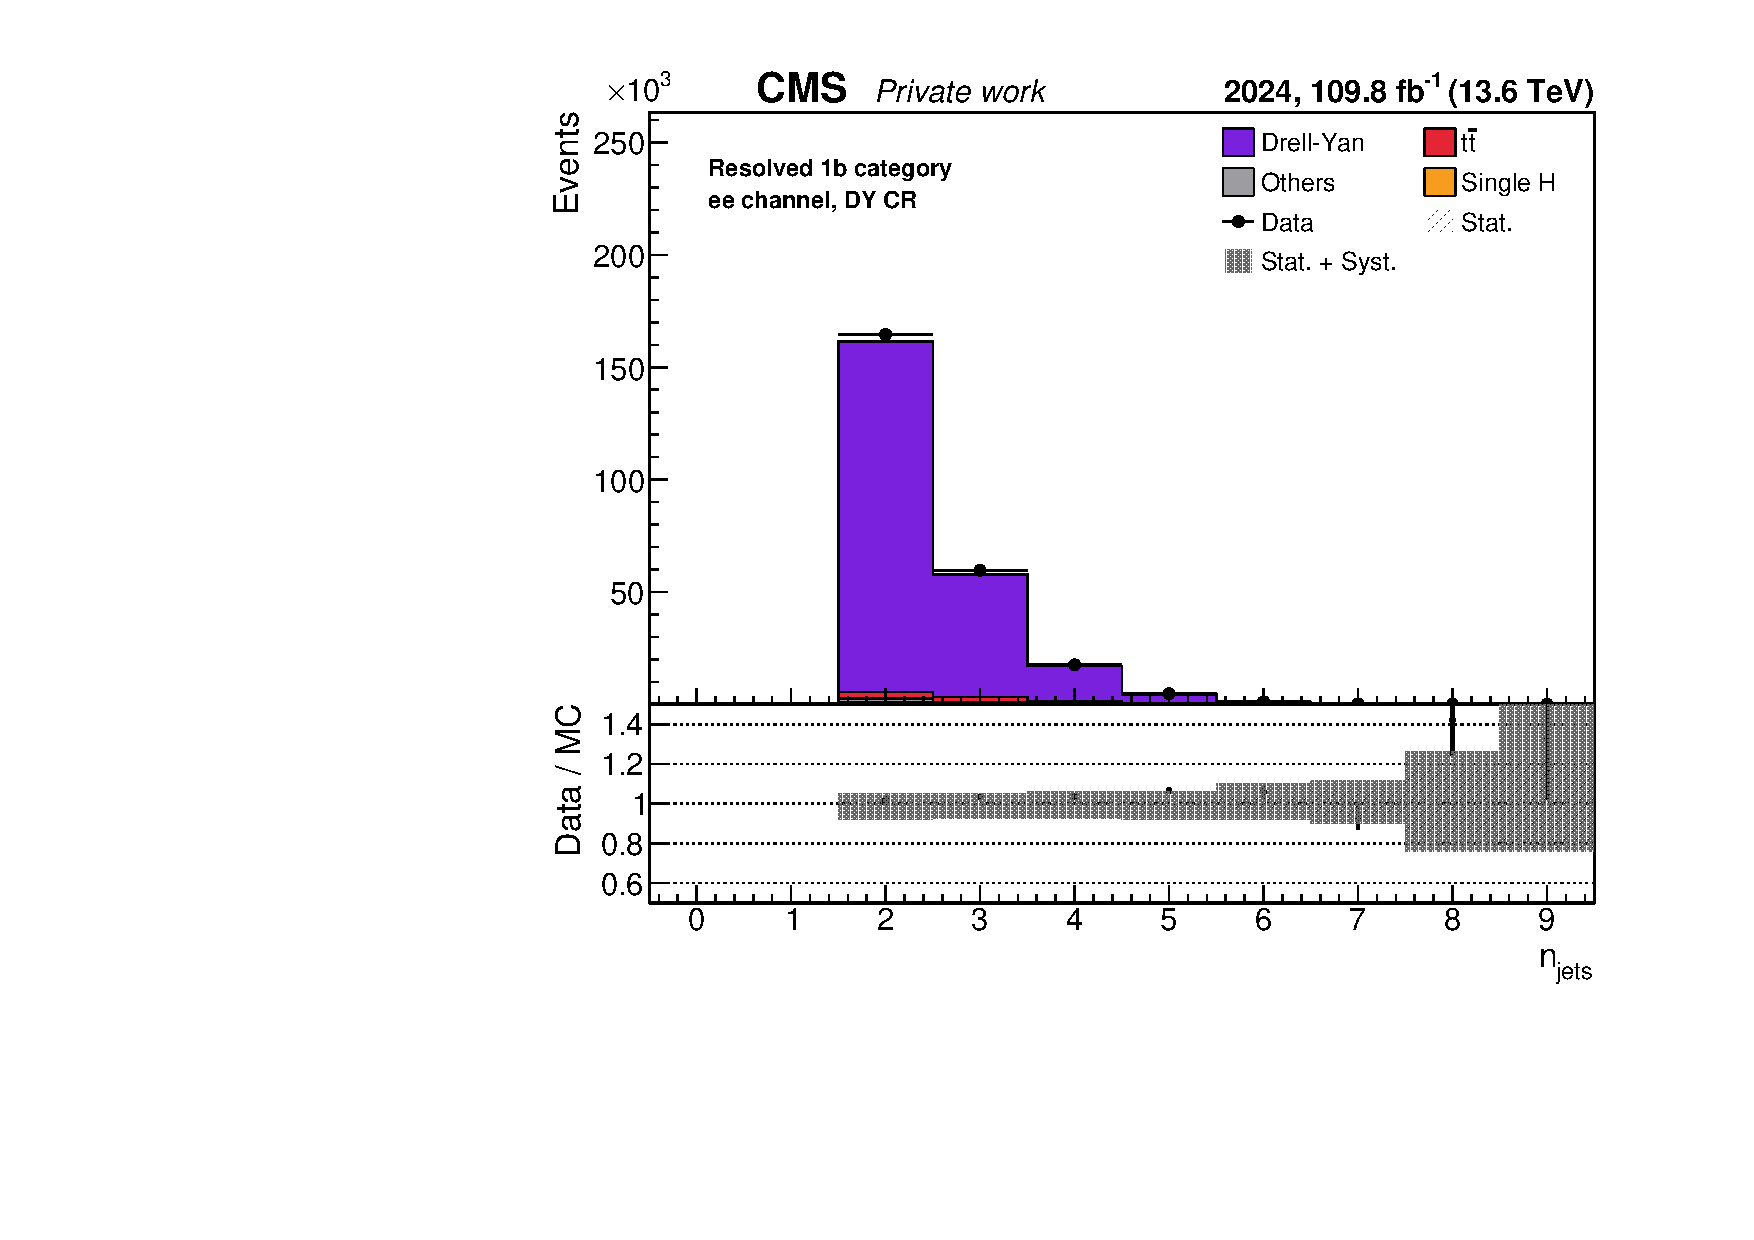
\includegraphics[width=0.49\linewidth, trim=11bp 0bp 40bp 14bp, clip]{figures/chapter_V/CR_res1b/THESIS_CR_DYCR_Prod_26_04_thesis/nCentralJets__ee_os_iso_DYCR__pg_forPlotsCR__stack.pdf}\\[2mm]
    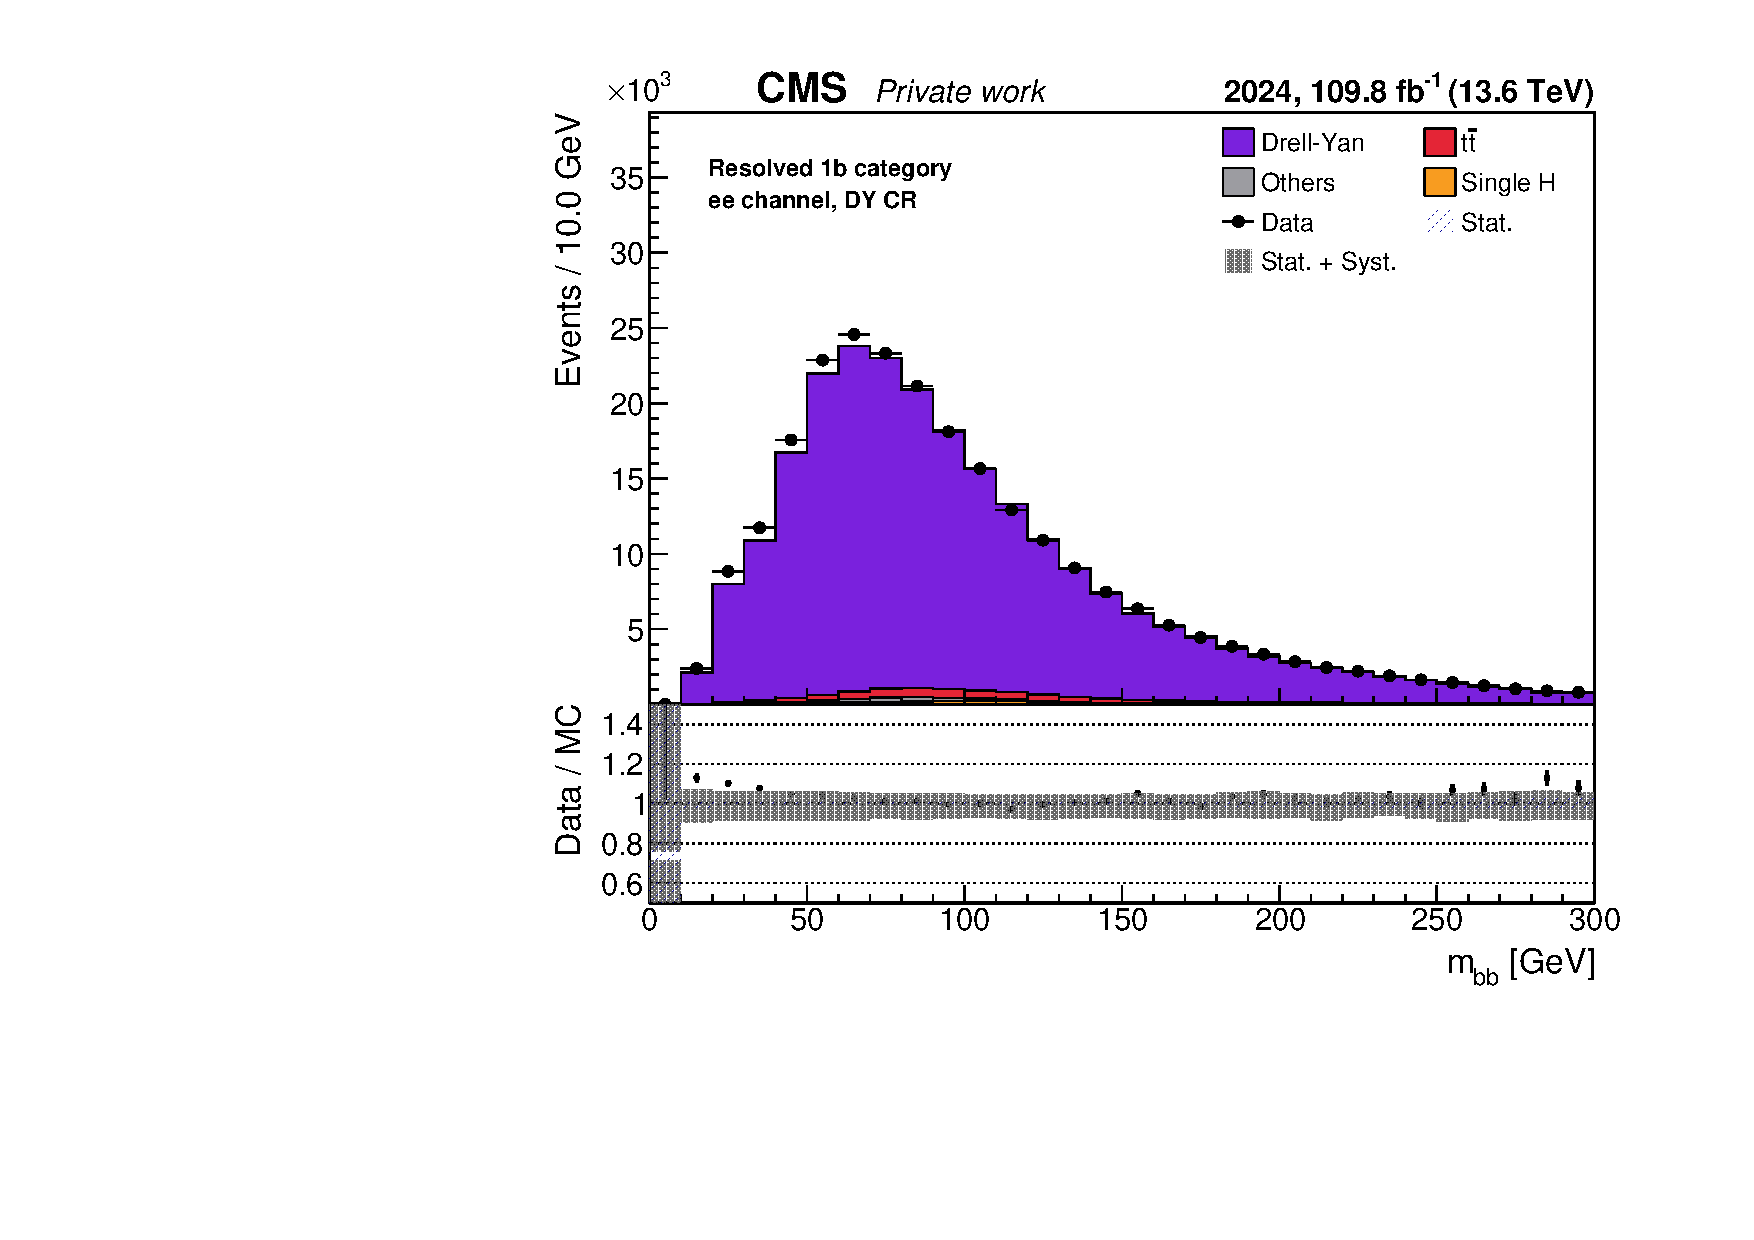
\includegraphics[width=0.49\linewidth, trim=11bp 0bp 40bp 14bp, clip]{figures/chapter_V/CR_res1b/THESIS_CR_DYCR_Prod_26_04_thesis/Hbb_mass__ee_os_iso_DYCR__pg_forPlotsCR__stack.pdf}\hfill
    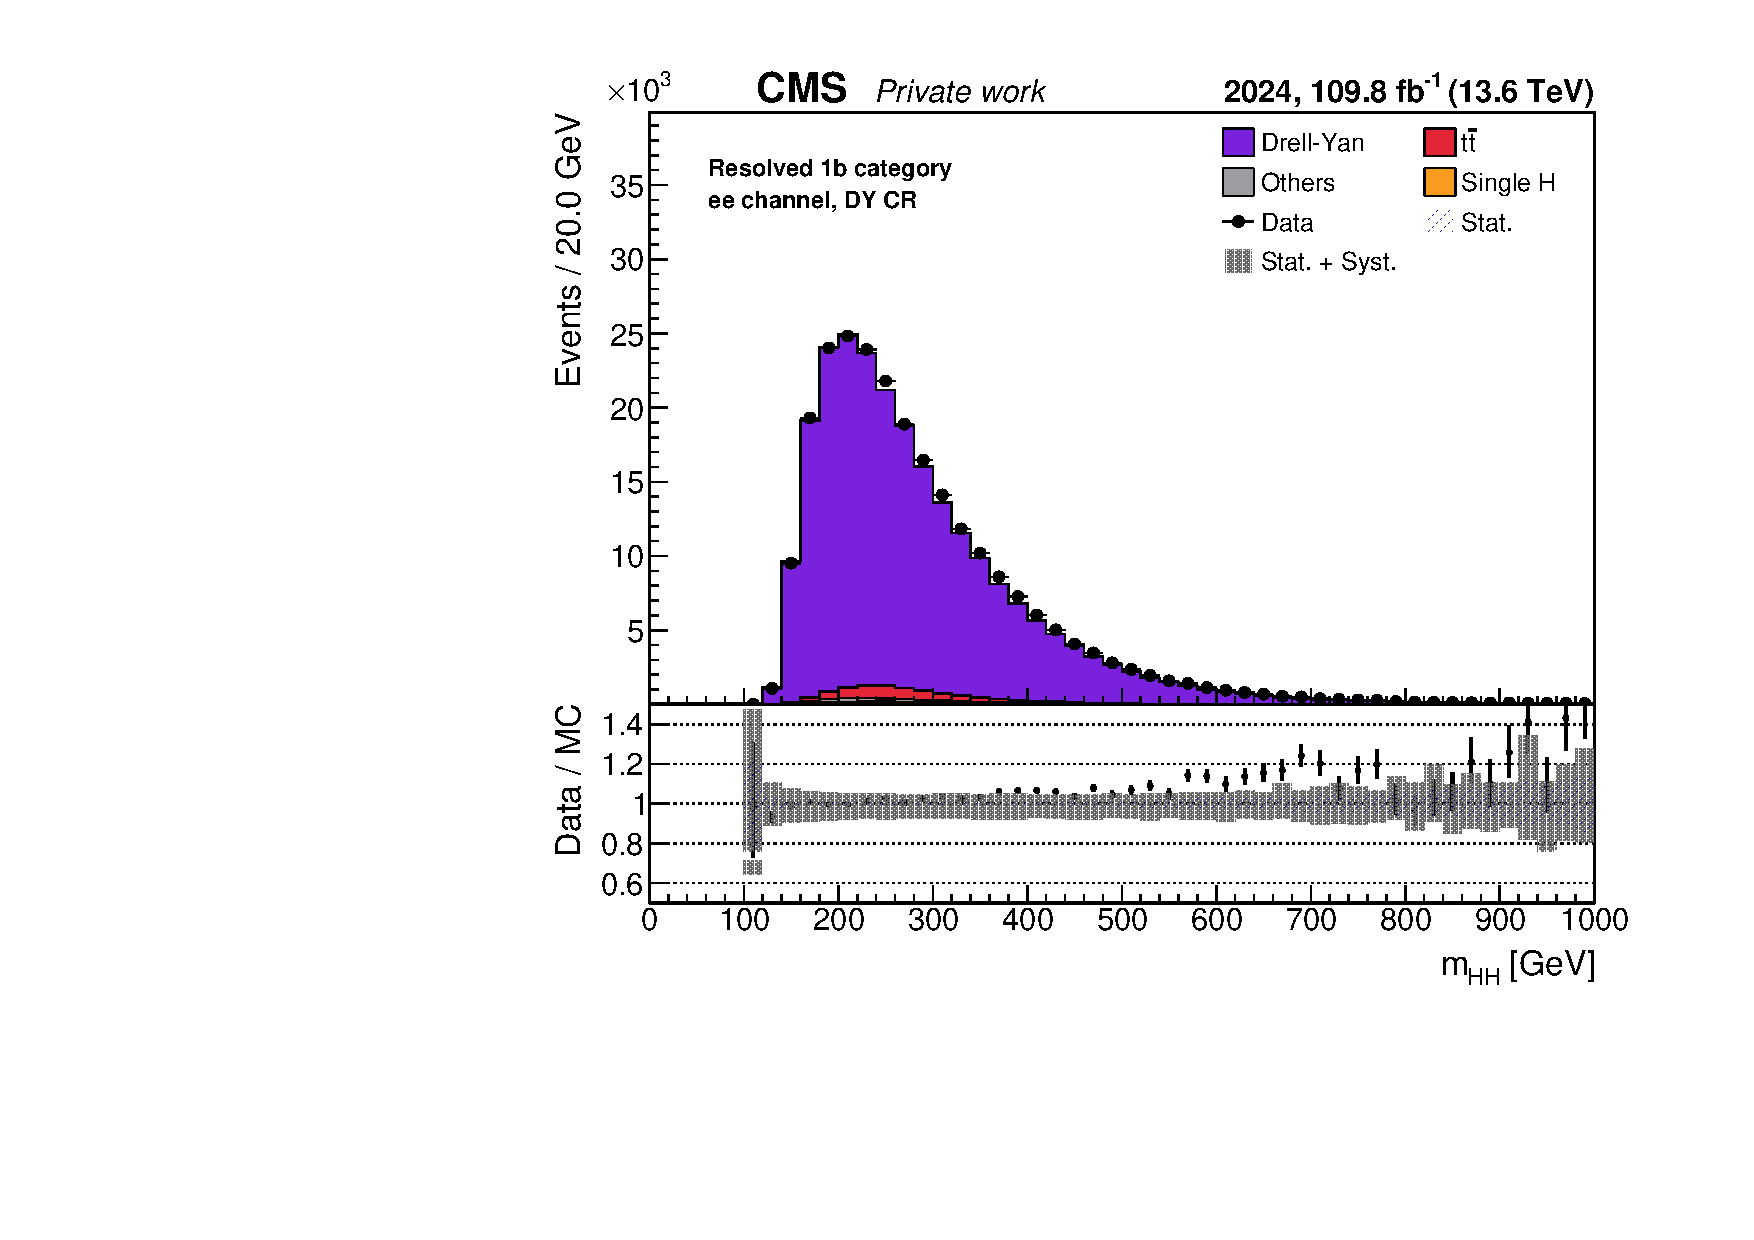
\includegraphics[width=0.49\linewidth, trim=11bp 0bp 40bp 14bp, clip]{figures/chapter_V/CR_res1b/THESIS_CR_DYCR_Prod_26_04_thesis/HH_mass__ee_os_iso_DYCR__pg_forPlotsCR__stack.pdf}
    \caption[Data and prediction in the Drell--Yan control region]{%
        Data and prediction in the Drell--Yan-enriched control region described in
        Section \ref{subsec:bbtt_cr}, in 2024: $p_T$ of the lepton pair (top left), number of
        jets (top right), mass of the $H\to b\bar{b}$ candidate (bottom left), and mass of the
        $HH$ system (bottom right). The band shows the statistical and systematic uncertainty
        of the prediction.}
    \label{fig:cr_dy}
\end{figure}
%
\begin{figure}[tbp]
    \centering
    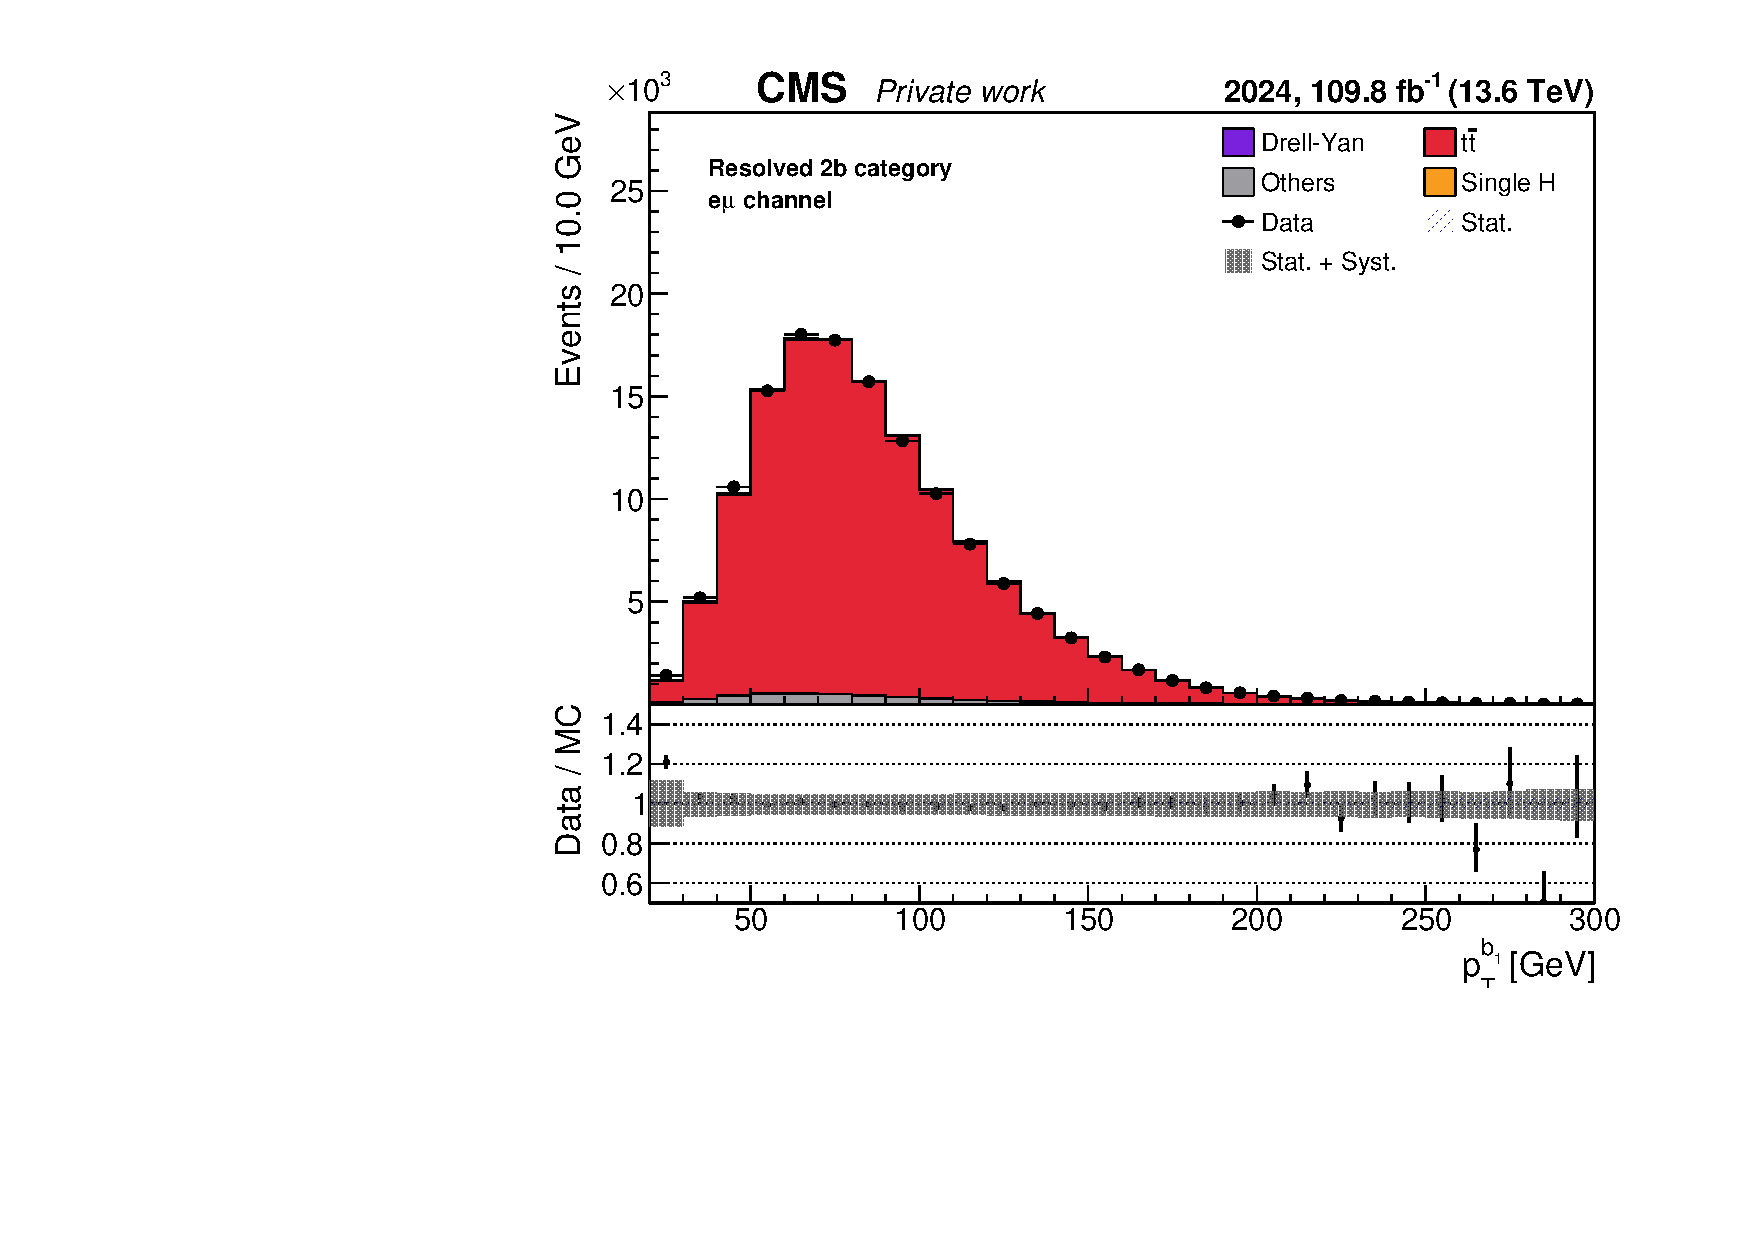
\includegraphics[width=0.49\linewidth, trim=11bp 0bp 40bp 14bp, clip]{figures/chapter_V/CR_res2b/THESIS_CR_Prod_26_04/bjet1_pt__emu_os_iso__pg_forPlotsCR__stack.pdf}\hfill
    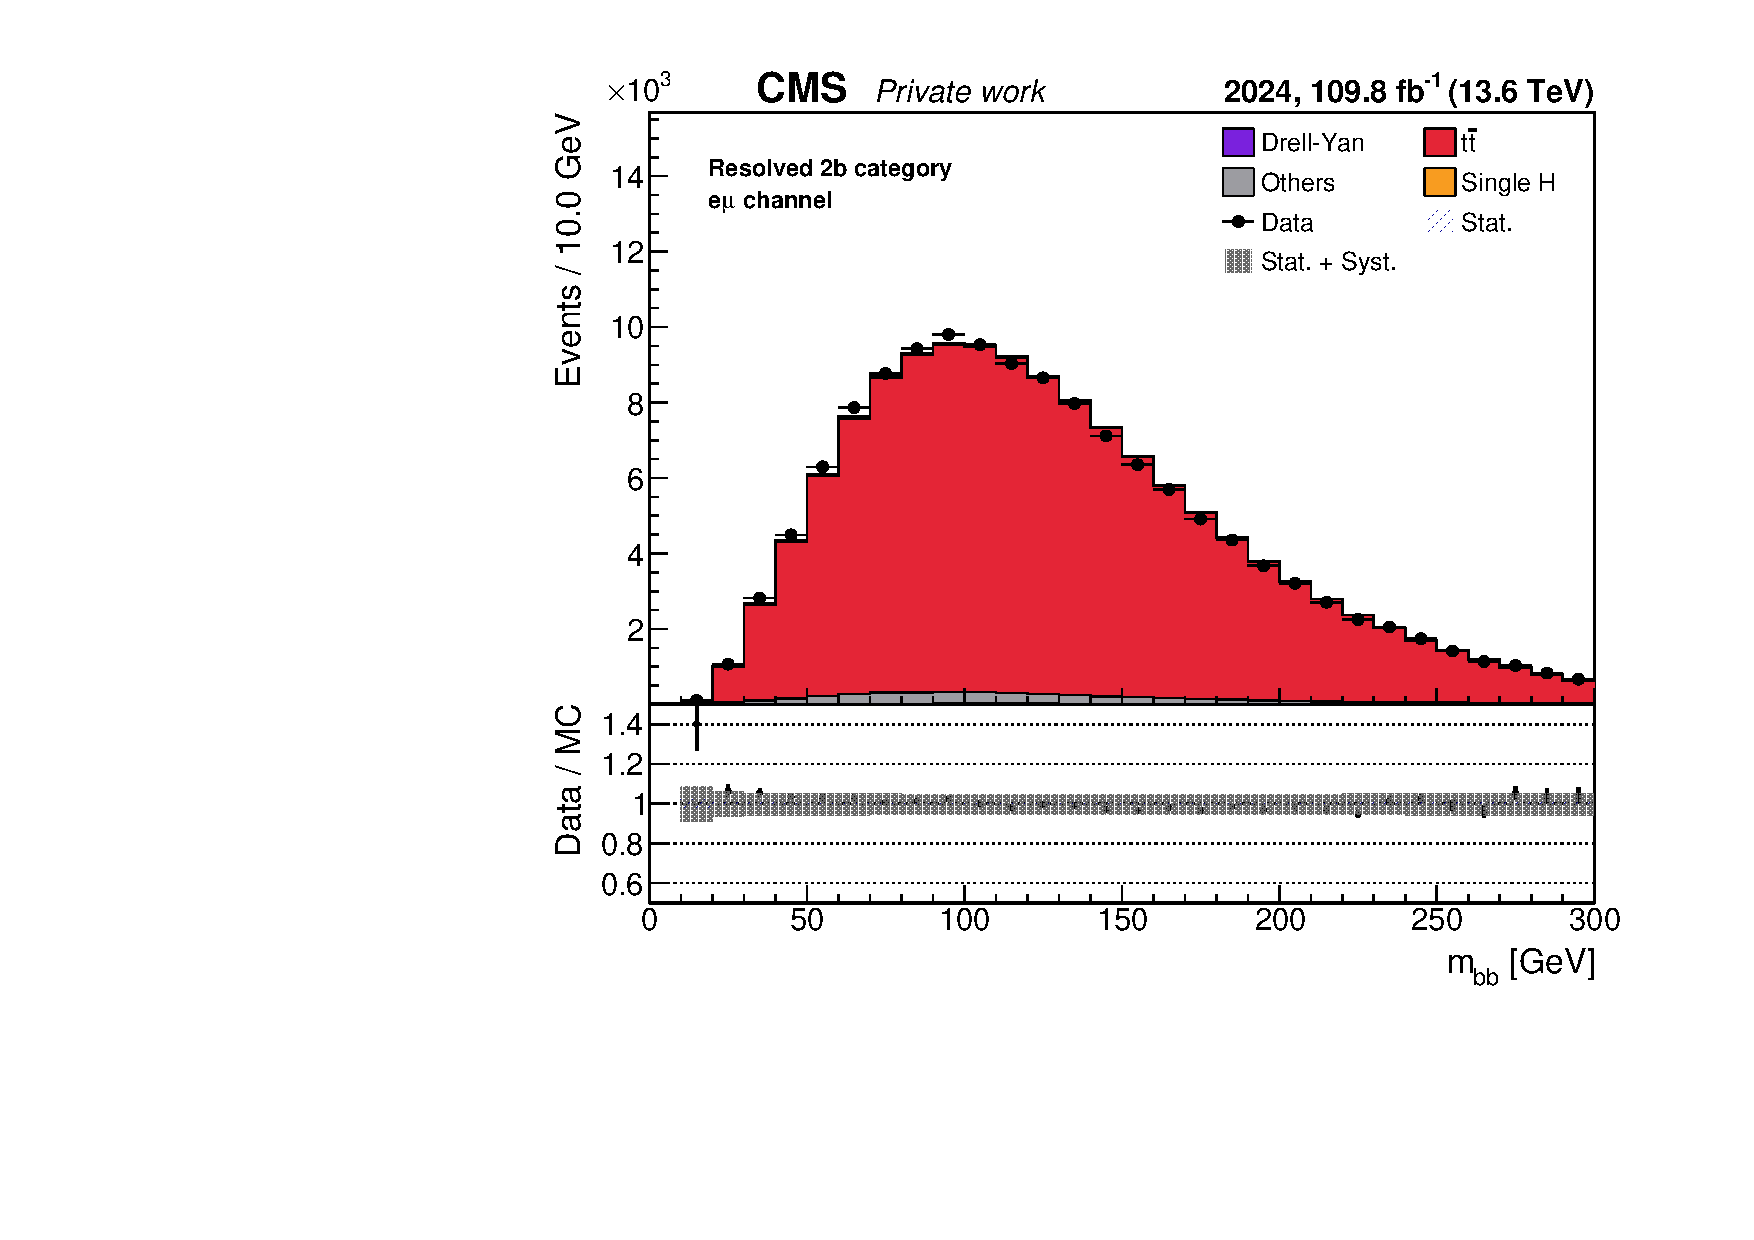
\includegraphics[width=0.49\linewidth, trim=11bp 0bp 40bp 14bp, clip]{figures/chapter_V/CR_res2b/THESIS_CR_Prod_26_04/Hbb_mass__emu_os_iso__pg_forPlotsCR__stack.pdf}\\[2mm]
    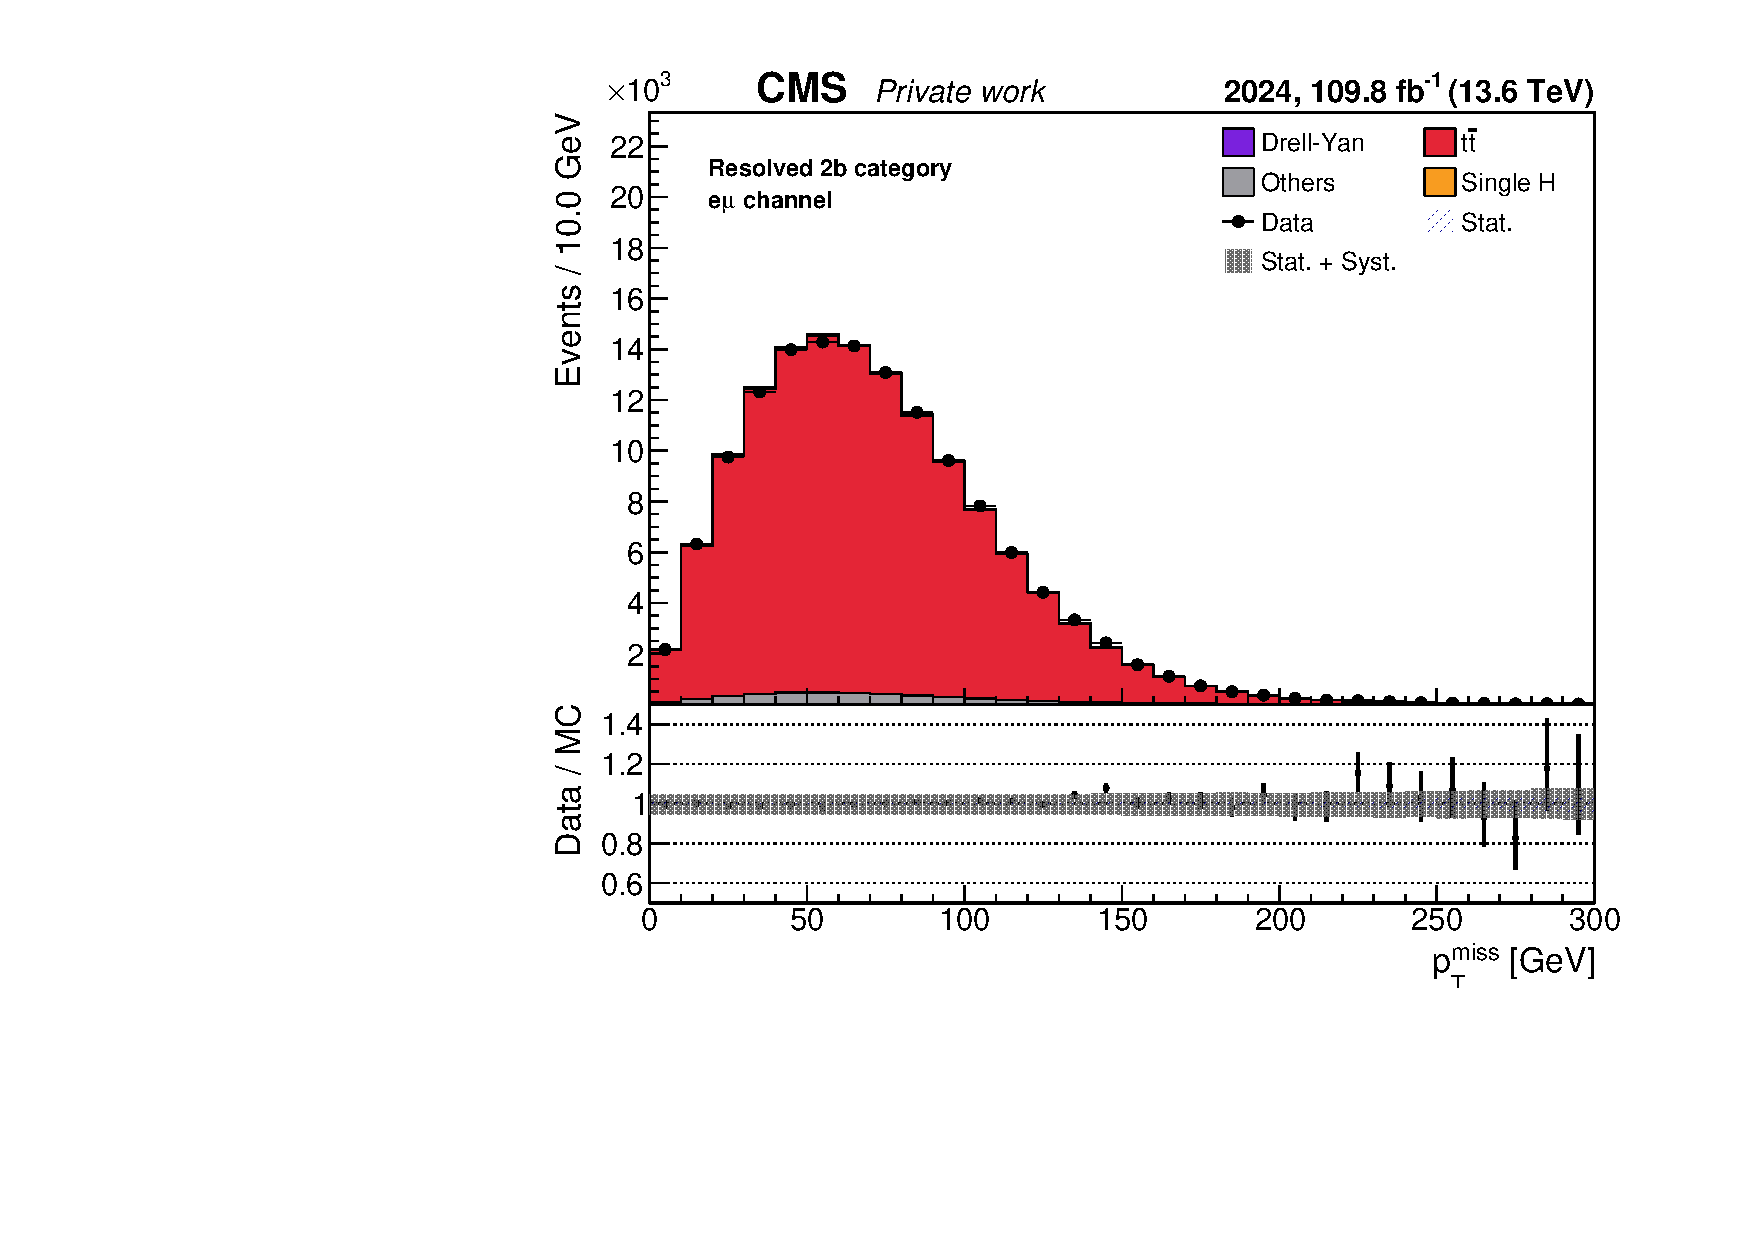
\includegraphics[width=0.49\linewidth, trim=11bp 0bp 40bp 14bp, clip]{figures/chapter_V/CR_res2b/THESIS_CR_Prod_26_04/PuppiMET_smeared_xycorr_pt__emu_os_iso__pg_forPlotsCR__stack.pdf}\hfill
    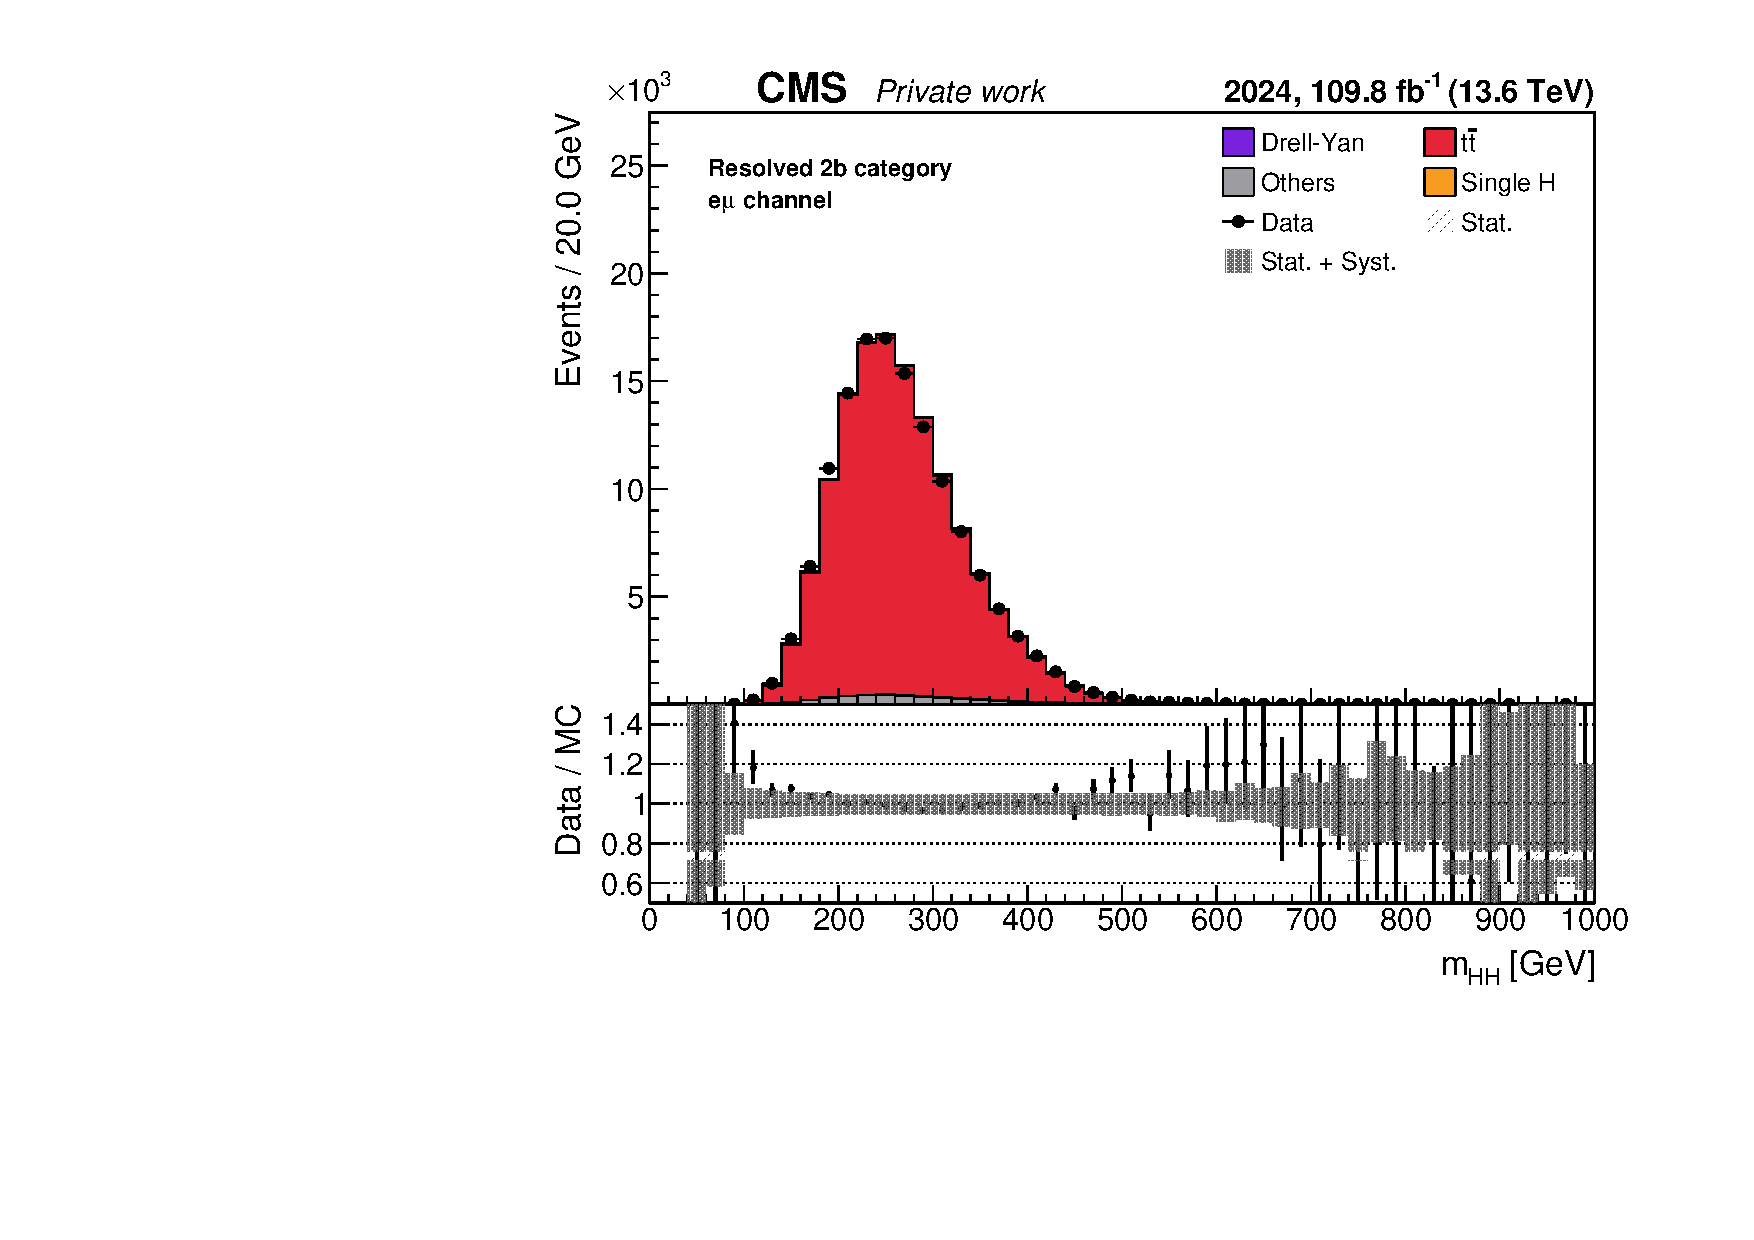
\includegraphics[width=0.49\linewidth, trim=11bp 0bp 40bp 14bp, clip]{figures/chapter_V/CR_res2b/THESIS_CR_Prod_26_04/HH_mass__emu_os_iso__pg_forPlotsCR__stack.pdf}
    \caption[Data and prediction in the $t\bar{t}$ control region]{%
        Data and prediction in the $t\bar{t}$-enriched control region described in
        Section \ref{subsec:bbtt_cr}, in 2024: $p_T$ of the leading $b$ jet (top left), mass of
        the $H\to b\bar{b}$ candidate (top right), $p_T^\text{miss}$ (bottom left), and mass of
        the $HH$ system (bottom right), with the same conventions as in Figure \ref{fig:cr_dy}.}
    \label{fig:cr_tt}
\end{figure}






\subsection{Distributions in the categories of the analysis}
%
Once the corrected simulation of the two dominant backgrounds and the fake factor method have been validated, the complete prediction is compared with the data in the categories of the analysis. Figure \ref{fig:prefit_mHH} shows the distribution of the reconstructed mass of the $HH$ system, the observable that most directly captures the kinematics of pair production, in the res2b category, which contributes most to the sensitivity of the analysis as shown in Section \ref{sec:bbtt_results}, for the four channels. Figure \ref{fig:prefit_cats} shows the same observable in the remaining categories for the $\tau_h\tau_h$ channel EN LAS VBF Y BOOSTED CATEGORIAS ES EL XTAUTAU. The distributions of other observables, categories, and channels are collected in Appendix \ref{app:prefit}.
\begin{figure}[tbp]
    \centering
    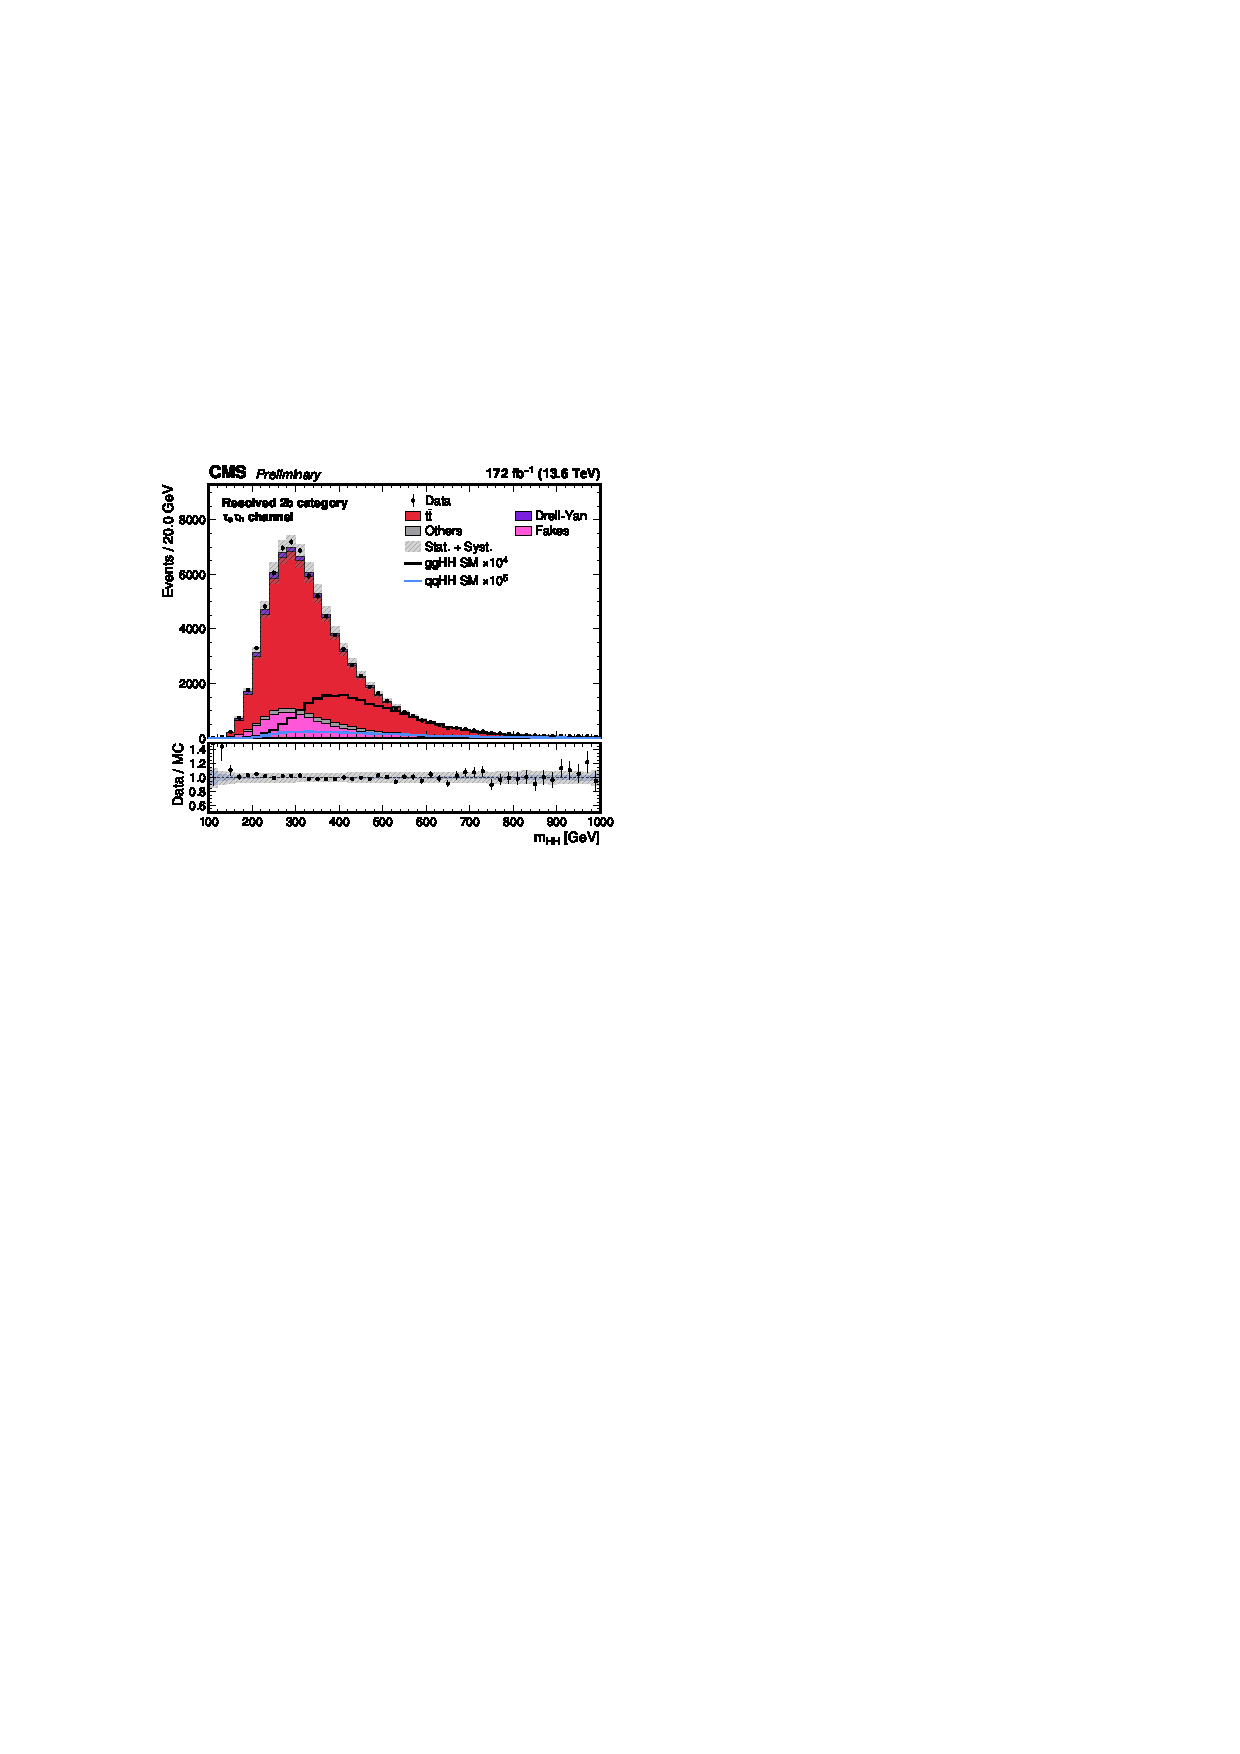
\includegraphics[width=0.49\linewidth]{figures/chapter_V/prefit_mHH_etau.pdf}
    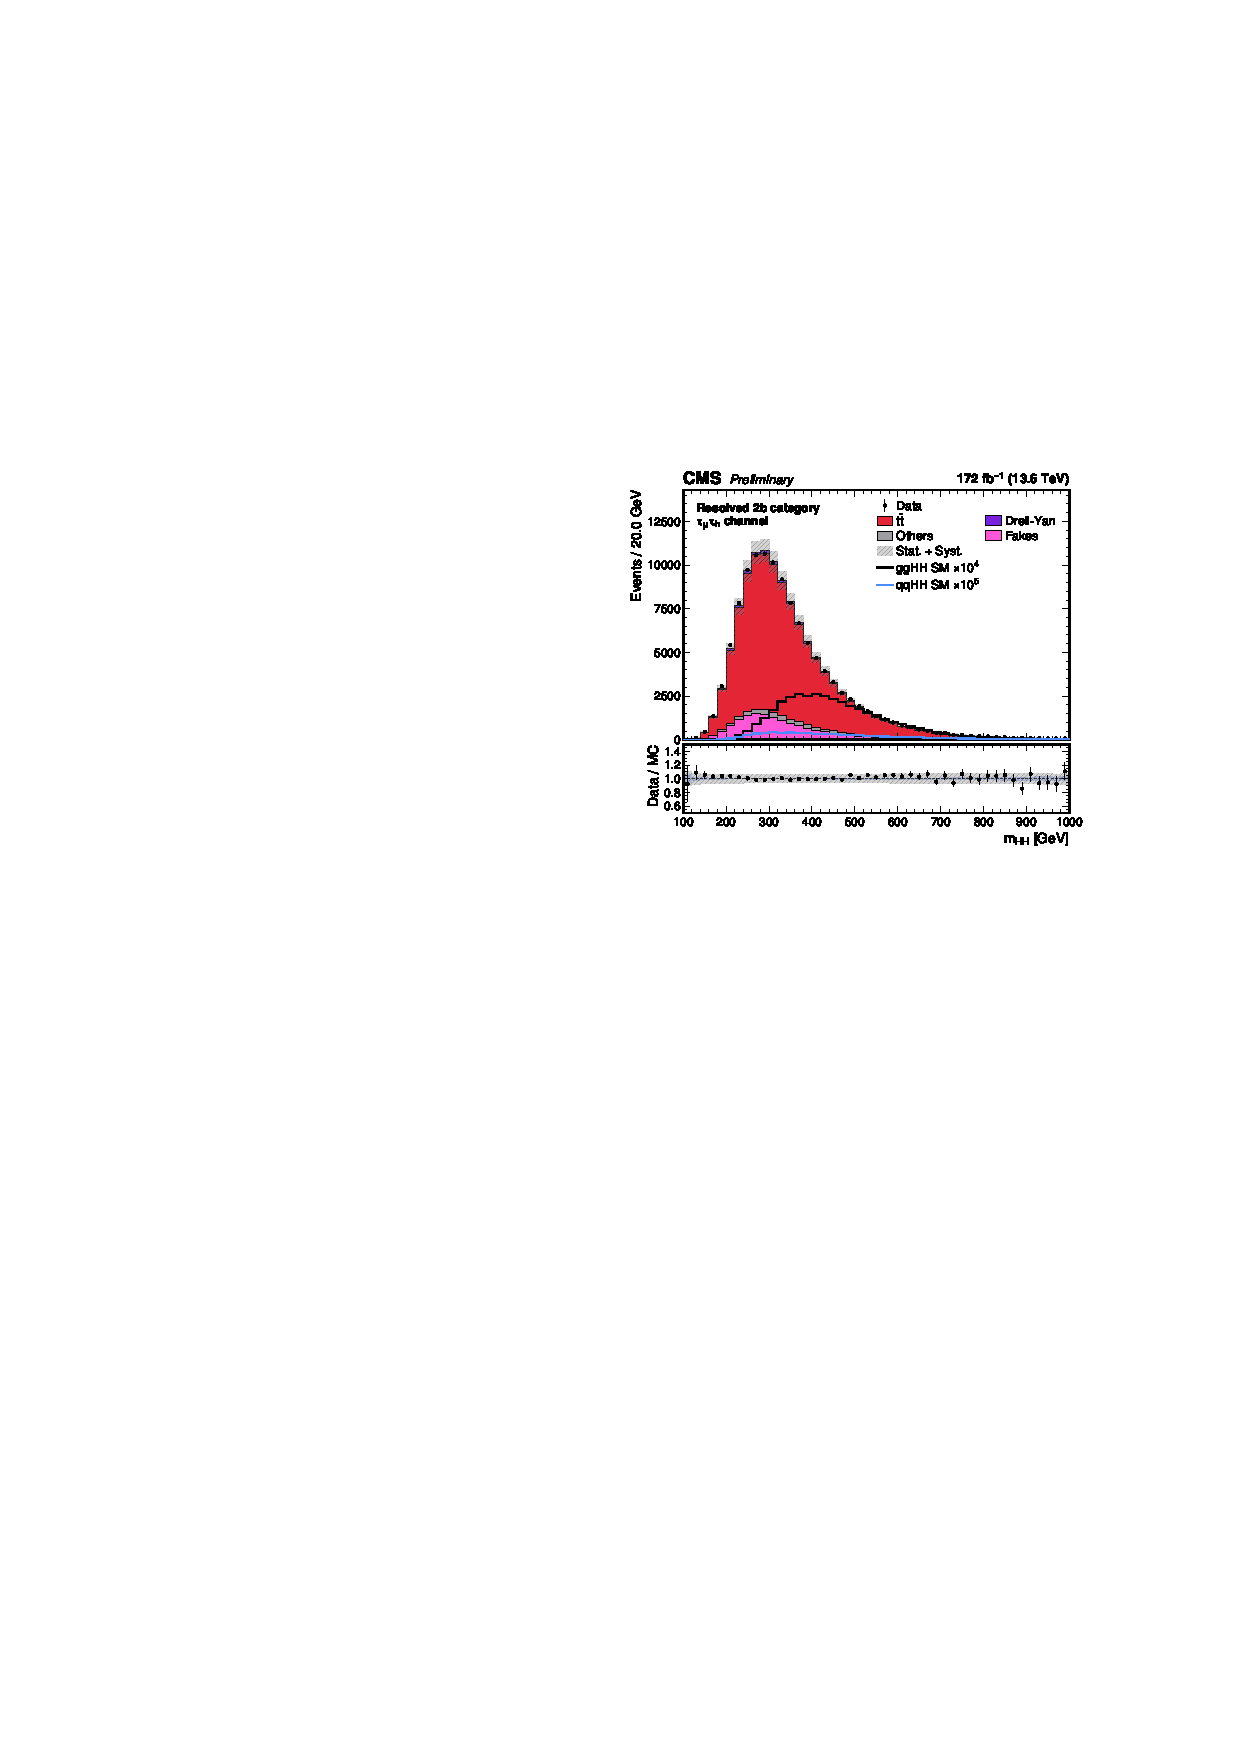
\includegraphics[width=0.49\linewidth]{figures/chapter_V/prefit_mHH_mutau.pdf}\\
    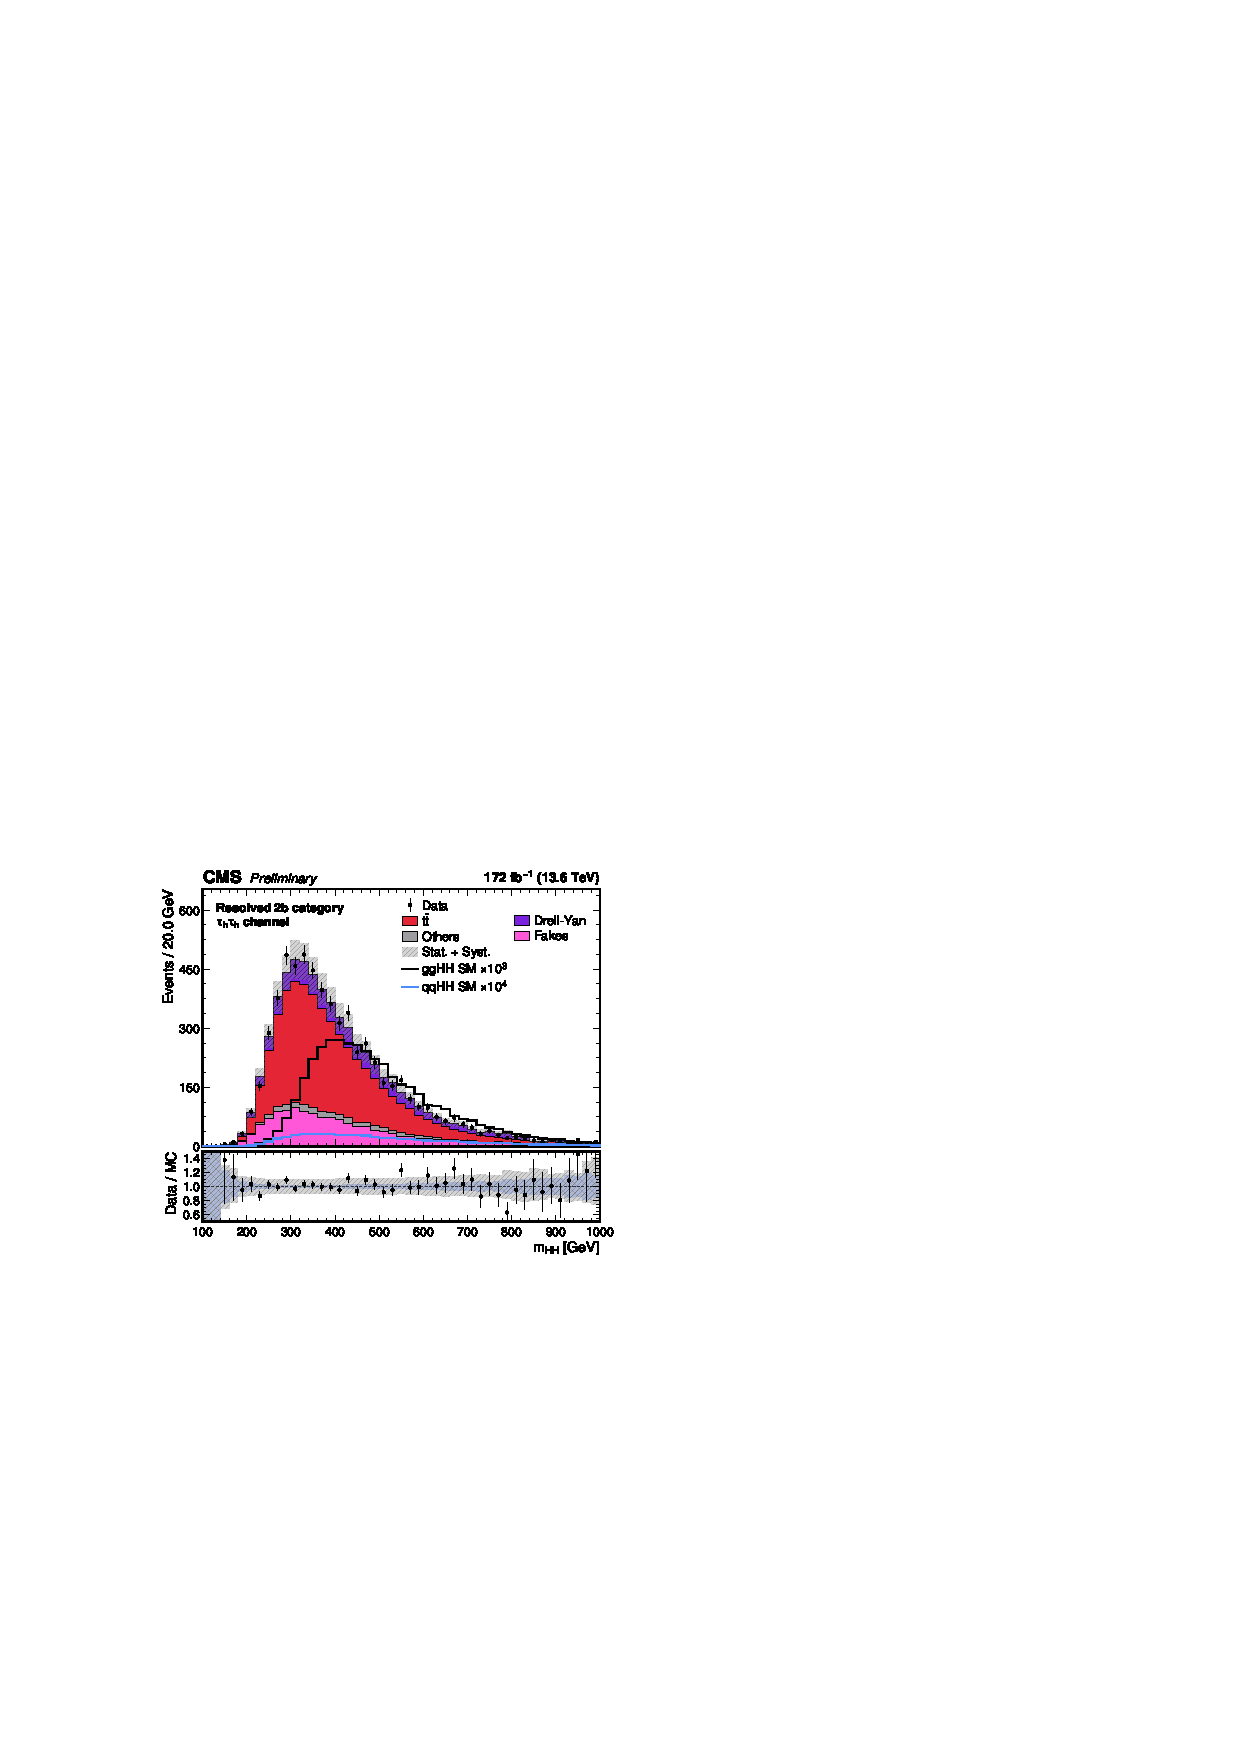
\includegraphics[width=0.49\linewidth]{figures/chapter_V/prefit_mHH_tautau.pdf}
    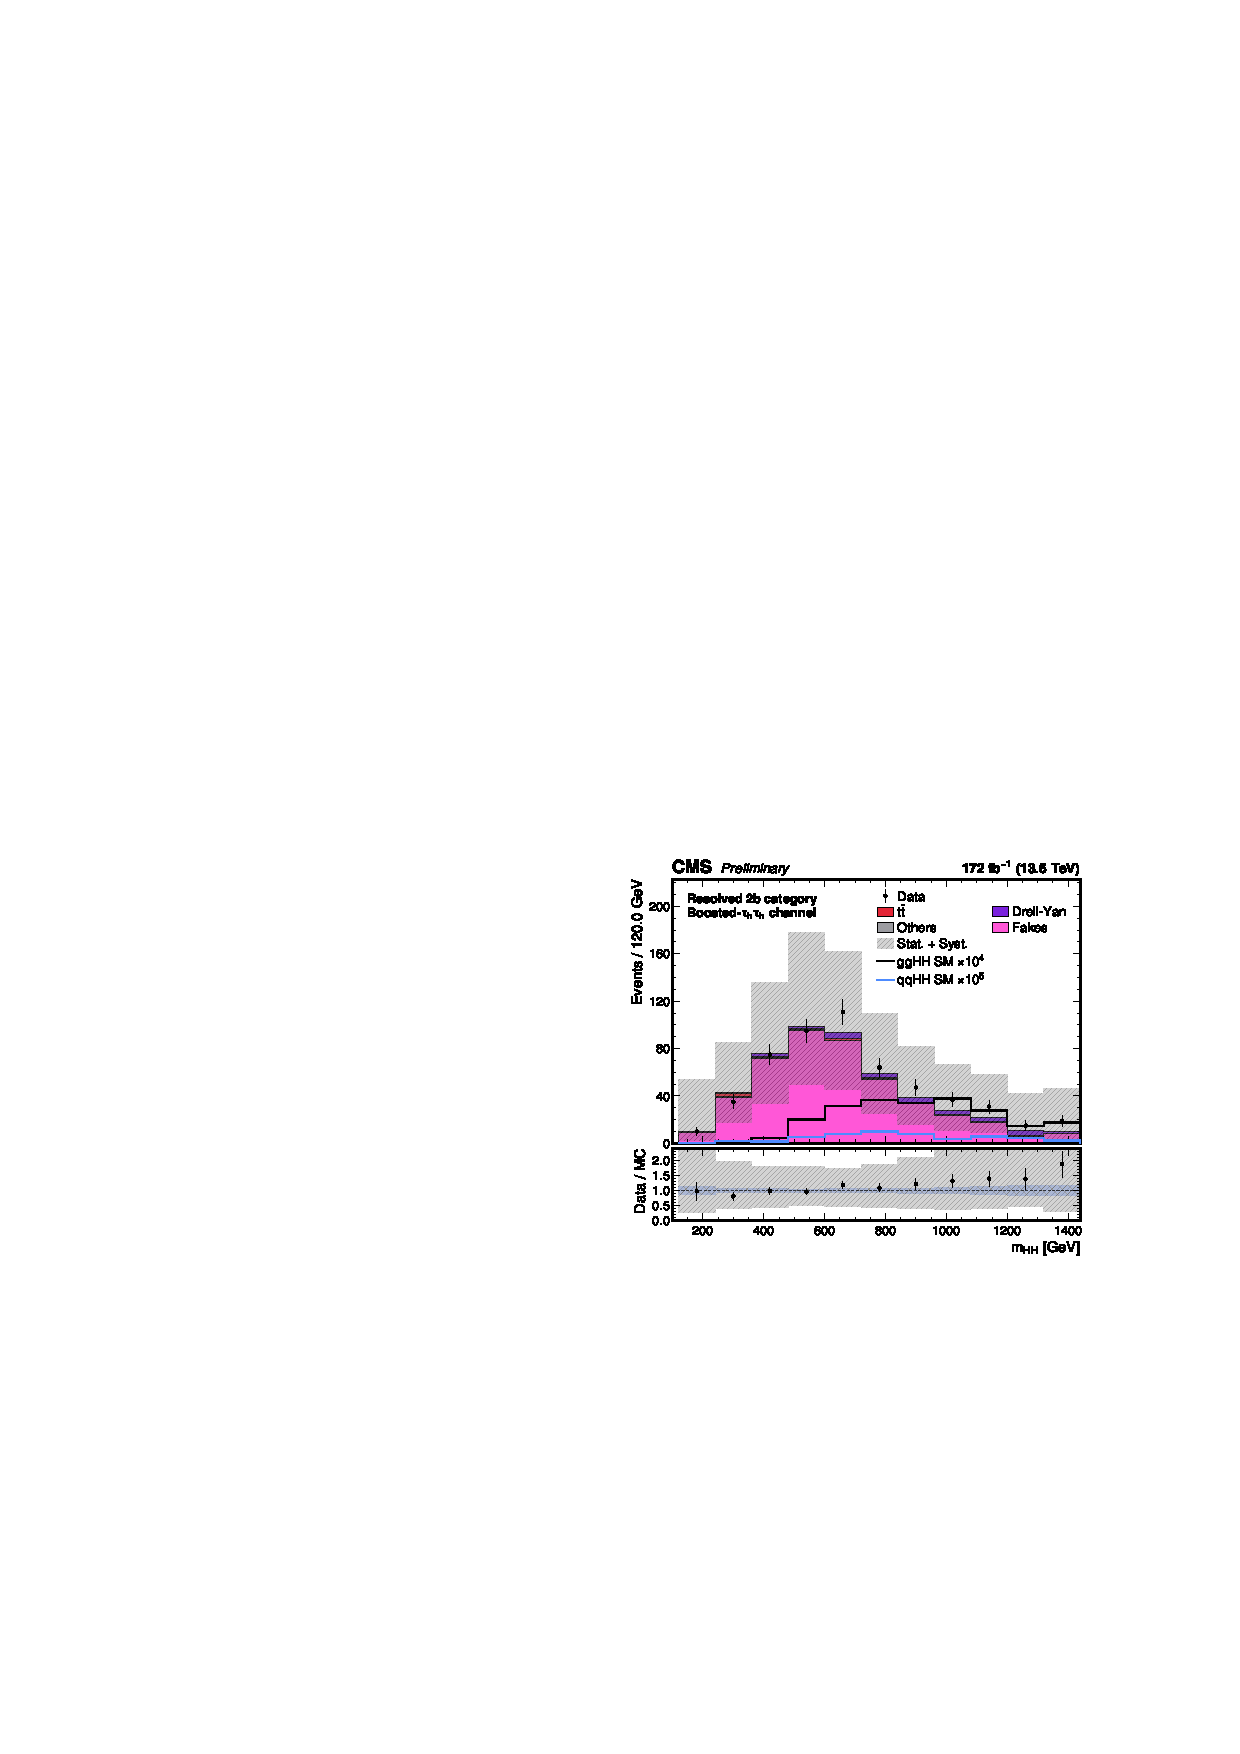
\includegraphics[width=0.49\linewidth]{figures/chapter_V/prefit_mHH_boosted.pdf}
    \caption[Pre-fit distributions of $m_{HH}$ in the res2b category]{%
        Distributions of the reconstructed mass of the $HH$ candidate, $m_{HH}$, in the
        res2b category, prior to fitting the data. The channels shown are       
        $\tau_e\tau_h$ (top left), $\tau_\mu\tau_h$ (top right),
        $\tau_h\tau_h$ (bottom left), and $b\tau_h\tau_h$ (bottom right),
        for the complete 2022–2024 dataset. The signal is plotted
        multiplied by the factors indicated in the legend. The shaded band
        represents the total statistical and systematic uncertainty of the prediction.
        Taken from Ref.~\cite{CMS-PAS-HIG-25-008}. SUSTITUIR POR LA QUE HE GENERADO YO}
    \label{fig:prefit_mHH}
\end{figure}
\begin{figure}[tbp]
    \centering
    % TODO: replace each \fbox with the m_HH plot of the category
    \fbox{\parbox[c][0.26\linewidth][c]{0.30\linewidth}{\centering res1b}}\hfill
    \fbox{\parbox[c][0.26\linewidth][c]{0.30\linewidth}{\centering boosted}}\hfill
    \fbox{\parbox[c][0.26\linewidth][c]{0.30\linewidth}{\centering VBF}}
    \caption[Pre-fit distributions of $m_{HH}$ in the other categories]{%
        Distributions of $m_{HH}$ before the fit in the res1b (left), boosted (middle), and
        VBF (right) categories of the $\tau_h\tau_h$ channel, with the same conventions as in
        Figure \ref{fig:prefit_mHH}.}
    \label{fig:prefit_cats}
\end{figure}


As expected, the composition of the background varies from one channel to another. While in the $\tau_e\tau_h$ and $\tau_\mu\tau_h$ channels the prediction is dominated by the production of top quark pairs, with smaller contributions from Drell--Yan and misidentified jets, in the $\tau_h\tau_h$ channel the fraction of fakes is considerably higher, although $t\bar{t}$ production remains the main contribution. The contribution from fakes becomes notably dominant in the $b\tau_h\tau_h$ channel, which has a much smaller number of events and where high $p_T$ jets are abundant in the multi-jet production. In all cases, the ratio between the data and the prediction is consistent with unity within the uncertainty band, with statistical fluctuations concentrated in the less populated tails. Therefore, the background is well modeled where the signal is indistinguishable from it, and the residual differences — consistent with the uncertainties described in Section \ref{sec:bbtt_systematics} — will be accounted for by the corresponding nuisance parameters in the final fit.\medskip

Beyond the data-to-prediction agreement, these distributions demonstrate that the signal only becomes visible in the figures when multiplied by factors ranging from $10^2$ to $10^5$, depending on the panel. Even in the most sensitive category and in the observable that best captures the kinematics of the $HH$ system, Higgs boson pair production contributes a fraction on the order of $10^{-4}$ of the total number of events, well below the statistical uncertainty of the data at any bin. \textcolor{red}{This holds for the SM signal, and also for the scenarios with modified couplings that remain allowed, since current searches already constrain the $HH$ cross section to a few times its SM value.ESTO REFORMULARLO CUANDO TENGA LOS PLOTS CON LAS SEÑALES}

No single variable allows the signal to be isolated on its own, and its extraction requires combining information from many of them into a single observable that maximizes the separation between signal and background. The construction of this discriminant is the subject of the following section.





% Section of its own, separate from the systematics (as Jaime does): here what is
% applied, in Sec. 6.10 what is assigned as an uncertainty on it.
% Pileup reweighting; L1 prefiring; trigger SFs; lepton reconstruction, ID and
% isolation SFs; tau_h ID and energy scale; b-tagging efficiency SFs; JES/JER.
% -> code: Corrections/{TAU,JME,LUM,MUO,EGM,BTV}


% Also a section of its own. Pre-fit data/MC in the baseline and in the control
% regions, per channel and per period; m_HH and pT_HH in resolved 2b are the
% representative pair (Figs. 2-3 of the PAS) because they separate signal best.
% State that residual discrepancies are covered by the systematics and absorbed
% by the fit -- do not leave the reader to wonder.
% -> code: scripts/make_CR_plots_*.sh, Category("FFvalidation_CR")


\section{Signal extraction}
\label{sec:bbtt_extraction}
%
Combining the relevant information into a single number is a classification problem, in which each event is assessed by how closely its properties resemble those of the signal or of the background. It is addressed with neural networks trained on simulated signal and background events, which return for each event a continuous score that accumulates signal events toward one end and background events toward the other.

The network assigns a score to every event entering a category, so that the data and each of the contributing processes have a distribution along that axis, and the measurement compares, bin by bin, the observed yield with the sum of those distributions. Within the fitted range, which starts at a score of $0.75$ (Section \ref{subsec:bbtt_rebinning}), the lowest bins are dominated by background and constrain the normalization of the processes that populate them, while the highest bins — where the signal is concentrated — provide the sensitivity of the analysis.

Signal extraction relies on two separately trained classifiers, each optimized for one production mode. The one dedicated to vector boson fusion is applied exclusively in the VBF category, and the one dedicated to gluon fusion in the remaining nine, so that the events of each category are scored by the network matched to the topology selected there. Both have three output nodes, associated with the signal, Drell--Yan, and $t\bar{t}$ production, of which only the signal node, referred to as the $HH$ score, is used in the fit.\medskip

The following subsections describe the architecture and inputs of the classifiers, their training and performance, and the binning of their output in the fit.


\subsection{Architecture and input variables}
%
Both classifiers follow the structure illustrated in Figure \ref{fig:dnn_architecture}, in which two networks generate variables from the inputs and a third one classifies the event from them. The first is a \textit{Lorentz Boost Network}~\cite{LBN}, whose objective is to process the input variables so that the network does not have to learn the relevant invariant combinations from scratch, but is instead directly provided with a set of them that have physical meaning. The Lorentz Boost Network is designed to process the four-momenta of the reconstructed objects and learns two sets of linear combinations of them: one forming new four-momenta and the other a reference frame in which they are evaluated. From the transformed four-momenta it extracts quantities that are passed to the rest of the model, so that the network is provided with combinations that have a kinematic meaning instead of having to learn them freely from the components $(E, p_x, p_y, p_z)$.

The second is the neutrino momentum regression network described in Section \ref{sec:bbtt_flow}, which estimates the momenta of the neutrinos from the $\tau$ decays using the kinematics of the event, including $p_T^\text{miss}$ and its covariance. In the gluon fusion classifier it is part of the model, so that $p_T^\text{miss}$ enters the classifier directly. The vector boson fusion classifier instead receives the neutrino momenta already estimated by a standalone version of the same network, and builds its $H\to\tau\tau$ candidate and $HH$ system with them. In both cases the information of $p_T^\text{miss}$ reaches the classification, in the second already processed into the reconstructed $\tau\tau$ system.

The outputs of these networks are concatenated with the remaining inputs and fed to a densely connected network~\cite{DenseNet}, in which each layer receives the outputs of all preceding ones, so that the intermediate variables remain accessible at any depth. Its last layer has three nodes -- associated with the signal, Drell--Yan, and $t\bar{t}$ production -- with \textit{softmax} activation, so that each output is a continuous number between zero and one that measures the compatibility of the event with the corresponding class, and the three sum to one.\medskip
\begin{figure}[tbp]
\centering
\definecolor{archInBg}{HTML}{FDF0EA}\definecolor{archInLn}{HTML}{E59A80}
\definecolor{archNetBg}{HTML}{F6EEF5}\definecolor{archNetLn}{HTML}{B48BB2}
\definecolor{archOutBg}{HTML}{F0DADF}\definecolor{archOutLn}{HTML}{B07480}
\newcommand{\ffont}{\fontfamily{Nunito-TLF}\selectfont}
\begin{tikzpicture}[
    x=1mm, y=1mm, font=\ffont\footnotesize,
    inp/.style   = {draw=archInLn, line width=0.6pt, rounded corners=3pt, fill=white,
                    align=center, inner sep=2pt, text width=38mm, minimum height=13mm,
                    font=\ffont\scriptsize,
                    execute at begin node={\hyphenpenalty=10000\relax}},
    net/.style   = {draw=archNetLn, line width=0.6pt, rounded corners=3pt, fill=white,
                    align=center, inner sep=2pt, font=\ffont\footnotesize\bfseries\boldmath},
    res/.style   = {draw=archOutLn, line width=0.6pt, rounded corners=3pt, fill=white,
                    align=center, inner sep=2pt, minimum height=6mm, minimum width=16mm,
                    font=\ffont\footnotesize\bfseries\boldmath},
    ar/.style    = {-{Latex[length=1.8mm]}, draw=archNetLn!80!black, line width=0.6pt},
    note/.style  = {font=\ffont\scriptsize\itshape, text=archOutLn!80!black, align=center, inner sep=0pt},
    title/.style = {font=\ffont\footnotesize\bfseries\boldmath, text=#1!75!black, anchor=north, inner sep=0pt},
    block/.style = {draw=#1Ln, fill=#1Bg, line width=0.6pt, rounded corners=5pt,
                    inner xsep=3.5mm, inner ysep=3.5mm}
  ]
  % ================= inputs
  \node[inp] (i1) at (20, 15)  {Four-momenta of the reconstructed objects and of the systems they form};
  \node[inp] (i2) at (20, 0)   {Categorical variables, tagging scores, and high-level variables};
  \node[inp] (i3) at (20, -15) {$p_T^\text{miss}$ and its covariance, decay modes and charges of the $\tau$ candidates};
  \coordinate (itop) at ([yshift=4.5mm]i1.north);
  % ================= networks
  \node[net, text width=22mm, minimum height=13mm] (lbn) at (64, 15)  {Lorentz Boost\\ Network};
  \node[net, text width=22mm, minimum height=13mm] (reg) at (64, -15) {{\boldmath$\tau\tau$} regression\\ network};
  \node[draw=archNetLn, line width=0.6pt, rounded corners=3pt, fill=archNetLn!18!white,
        minimum width=6mm, minimum height=43mm] (cc) at (85, 0) {};
  \node[font=\ffont\scriptsize\bfseries, text=archNetLn!70!black, rotate=90] at (cc.center) {concatenation};
  \node[net, text width=14mm, minimum height=20mm] (dn) at (101, 0) {Dense\\ network};
  \coordinate (ntop) at ([yshift=4.5mm]lbn.north);
  % ================= outputs
  \node[res, draw=archOutLn!85!black, fill=archOutLn!45!white] (o1) at (136, 8) {$HH$};
  \node[res] (o2) at (136, 0)  {DY};
  \node[res] (o3) at (136, -8) {$t\bar{t}$};
  \node[note, anchor=south] (fitnote) at ([yshift=3mm]o1.north) {$HH$ score:\\ fitted observable};
  \coordinate (otop) at ([yshift=4.5mm]lbn.north -| o1);
  \coordinate (obot) at (i3.south -| o1);
  % ================= arrows
  \draw[ar] (i1.east) -- (lbn.west);
  \draw[ar] (i3.east) -- (reg.west);
  \draw[ar] (i2.east) -- (i2.east -| cc.west);
  \draw[ar] (lbn.east) -- (lbn.east -| cc.west);
  \draw[ar] (reg.east) -- (reg.east -| cc.west);
  \draw[ar] (cc.east) -- (dn.west);
  \coordinate (fan) at (123, 0);
  \draw[draw=archNetLn!80!black, line width=0.6pt] (dn.east) -- (fan);
  \draw[ar] (fan) |- (o1.west);
  \draw[ar] (fan) -- (o2.west);
  \draw[ar] (fan) |- (o3.west);
  % ================= blocks
  \begin{pgfonlayer}{background}
    \node[block=archIn, fit=(itop)(i1)(i3)] (inblock) {};
    \node[block=archNet, fit=(ntop)(lbn)(reg)(cc)(dn)] (netblock) {};
    \node[block=archOut, fit=(otop)(o1)(o3)(fitnote)(obot)(fan)] (outblock) {};
  \end{pgfonlayer}
  \node[title=archInLn] at ([yshift=-2.5mm]inblock.north)  {INPUT FEATURES};
  \node[title=archNetLn] at ([yshift=-2.5mm]netblock.north) {NETWORKS};
  \node[title=archOutLn] at ([yshift=-2.5mm]outblock.north) {OUTPUTS};
\end{tikzpicture}
\caption[Architecture of the signal-extraction discriminants]{%
  Schematic representation of the architecture of the classifiers, showing which input
  features enter each network and the three output nodes, of which the $HH$ one provides the
  observable used in the fit (Section \ref{sec:bbtt_statistics}). In the vector boson fusion
  classifier, the $\tau\tau$ regression is not trained jointly, and its outputs enter as input
  features.}
\label{fig:dnn_architecture}
\end{figure}

The two classifiers differ in their training samples and inputs. The gluon fusion classifier is trained on the simulated backgrounds and on gluon fusion signal samples, without any category requirement, resulting in a single network covering the nine categories in which it is subsequently used. In contrast, the vector boson fusion classifier is trained on Drell--Yan, $t\bar{t}$, and signal samples of both production modes, in a loose version of the VBF category, which requires only $m_{jj} > 500$ GeV and $|\Delta \eta_{jj}| > 3$ for the VBF jet pair, and is therefore optimized for the VBF region.

The input variables of both classifiers are listed in Table \ref{tab:dnn_inputs}. They comprise the four-momenta of the reconstructed objects and of the systems they form — each of the two Higgs boson candidates and the $HH$ candidate; categorical variables that identify the channel, the decay mode and charge of each $\tau$ candidate, and whether the $H\to b\bar{b}$ candidate has been reconstructed in the resolved or merged topology; $p_T^\text{miss}$ and its covariance in the gluon fusion classifier, replaced in the vector boson fusion one by the regressed neutrino momenta; and the scores of the tagging algorithms, including the \textsc{HH-BTag} score presented in Chapter \ref{ch:taggers}, through which the work of the first part of this thesis feeds directly into the signal extraction. 
%
\begin{table}[tbp]
\centering
\small
\renewcommand{\arraystretch}{1.1}
\begin{tabular}{@{}ll>{\centering\arraybackslash}p{1.1cm}>{\centering\arraybackslash}p{1.1cm}@{}}
\toprule
Group & Variable & ggF & VBF \\
\midrule
Categorical       & Channel                                                      & $\bullet$ & $\bullet$ \\
                  & Decay modes and charges of the $\tau$ candidates             & $\bullet$ & $\bullet$ \\
                  & Presence of a $b$ jet pair and of a large-radius jet         & $\bullet$ & $\bullet$ \\
                  & Presence of a VBF jet pair                                   & --        & $\bullet$ \\
\midrule
Objects           & Four-momenta of the two $\tau$ candidates                    & $\bullet$ & $\bullet$ \\
                  & Four-momenta of the two $b$ jet candidates                   & $\bullet$ & $\bullet$ \\
                  & Four-momentum of the large-radius jet                        & $\bullet$ & $\bullet$ \\
                  & Four-momenta of the two VBF jets                             & --        & $\bullet$ \\
\midrule
Composite systems & Four-momenta of the $H\to\tau\tau$ and $H\to b\bar{b}$ candidates & $\bullet$ & $\bullet$ \\
                  & Four-momentum of the $HH$ system                             & $\bullet$ & $\bullet$ \\
\midrule
$p_T^\text{miss}$ & Transverse components and covariance matrix                  & $\bullet$ & --        \\
                  & Neutrino momenta from the $\tau\tau$ regression              & --        & $\bullet$ \\
\midrule
Tagging scores    & $b$, $c$ vs.\ $b$, and $c$ vs.\ light discriminants of the $b$ jets & $\bullet$ & $\bullet$ \\
                  & \textsc{HH-BTag} score of the $b$ jets                       & $\bullet$ & $\bullet$ \\
                  & Quark vs.\ gluon discriminant of the VBF jets                & --        & $\bullet$ \\
\midrule
High-level        & $M_\chi$ (Equation \ref{eq:mchi})                            & --        & $\bullet$ \\
                  & Mass and $\Delta R$ of the VBF jet pair                      & --        & $\bullet$ \\
                  & Products of the pseudorapidities of the $b$ and VBF jet pairs & --       & $\bullet$ \\
                  & Four Fox--Wolfram moments                                    & --        & $\bullet$ \\
\bottomrule
\end{tabular}
\caption[Input variables of the signal-extraction discriminants]{%
    Input variables of the gluon fusion and vector boson fusion discriminants. The
    four-momenta are rotated in the transverse plane so that the $\tau\tau$ pair is aligned
    with the $x$ axis. The gluon fusion classifier processes $p_T^\text{miss}$ and its
    covariance with the $\tau\tau$ regression network included in the model, whereas the
    vector boson fusion classifier receives the neutrino momenta already estimated by a
    standalone version of that network, with which its $H\to\tau\tau$ candidate and $HH$
    system are also built.}
\label{tab:dnn_inputs}
\end{table}


The vector boson fusion classifier additionally receives the four-momenta of the VBF jets and their quark versus gluon discriminant, together with high-level variables that condense information the network would have difficulty extracting from the low-level inputs. These are the mass and angular separation of the VBF jet pair; the products of the pseudorapidities of the two $b$ jet candidates and of the two VBF jets, which are negative when the two jets lie in opposite hemispheres; four Fox--Wolfram moments \cite{FoxWolfram}, which characterize the angular distribution of the hadronic activity; and the variable
%
\begin{equation}
    M_{\chi} = m_{bb\tau\tau} - \left(m_{bb} - m_H\right) - \left(m_{\tau\tau} - m_H\right),
    \label{eq:mchi}
\end{equation}
%
which corrects the reconstructed mass of the $HH$ system by subtracting the deviations of the masses of the two candidates from $m_H$, thereby compensating for the experimental resolution on both.

These high-level variables were selected iteratively from a broader list of discriminating variables identified in previous searches of this type. At each step, the network is trained, the loss of performance caused by permuting the values of each variable is evaluated, averaged over several repetitions, and the least influential variables are discarded before retraining, as in the procedure described in Section \ref{subsec:featimp}. Only the subset listed above survives.
% El código muestra cómo está montado, no el motivo. Una explicación plausible es que la red de VBF se desarrolló aparte y en otro formato (ONNX, frente al TensorFlow de la de ggF). Además, se entrena con pocos sucesos, en la región VBF, y reutilizar una regresión ya entrenada evita volver a aprenderla con tan poca estadística. Pero esto es una suposición. Si lo vas a poner en el texto, confírmalo con quien desarrolló la red de VBF.
% comprobacion: ggF: HHRun3DNNInterface.cc, función SetEventInputs (l.103–262). Ahí se construyen las entradas que se pasan al modelo: $p_T^\text{miss}$ ($p_x$, $p_y$ rotados), su covarianza (MET_covXX, covXY, covYY), los cuadrimomentos de los $\tau$, los $b$ y el jet grande, los scores de $b$ tagging, los sistemas compuestos y las variables categóricas.
% VBF: VBFONNXRuntimeInterface.cc, función GetVBFScoreFromInputs (l.124–195). Ahí están los dos vectores de entrada, el categórico y el continuo, variable por variable. No hay ninguna variable de $p_T^\text{miss}$, y sí aparecen nu1_px…nu2_pz, es decir, los momentos de los neutrinos.
% Regresión: en HHDNN.py (l.564–638) hay un modelo de regresión independiente (neutrino_regression_model_v0_24 para 2024 y v0_22-23 para 2022–2023). Se ejecuta antes que los clasificadores y guarda los momentos de los neutrinos en el ntuple. Esas variables son las que recibe la red de VBF, y también las que dan la masa $m_{\tau\tau}$ de la regresión que usa la elipse.
%




\subsection{Training and performance}
% 
Both classifiers are trained with a procedure similar to the one described in Section \ref{subsec:training} for the algorithms of Chapter \ref{ch:taggers}. The simulated events are divided into five subsets according to their event number, and a model is trained on four of them and evaluated on the fifth, so that every event is scored by a network that has not seen it during training. One quarter of the events of each training set is reserved for validation, and training stops when the loss on this subset no longer improves, which, together with a consistent evolution of the loss on the training set, ensures that the model learns general patterns rather than memorizing the training events.
%For the vector boson fusion classifier, several networks are trained for each subset from different initial values of their parameters, and the score is the average of their predictions, which reduces the dependence on any particular initialization \cite{CMS-PAS-HIG-25-008}.


The performance of the classifiers is evaluated with two complementary tools. The receiver operating characteristic (ROC) curve is built for each class against the other two by varying a threshold on the score of that class, and shows the fraction of events of the class above the threshold against the fraction of the other events that also pass it. The area under the curve summarizes it in a single number, equal to one for a perfect separation and to one half for a score without information. The confusion matrix, instead, assigns each event to the class whose output is highest, and the matrix shows, for the events of each true process (rows), the fraction assigned to each of the three classes (columns). The diagonal therefore gives the fraction of events correctly classified, and the off-diagonal elements show which processes the network tends to confuse. Figure \ref{fig:dnn_performance} shows both for the vector boson fusion classifier, as an example, evaluated on one of the five subsets, the others giving comparable results.
% 5-fold cross-validation; several random initialisations per fold; the final score
% is the average of the ensemble, which reduces dependence on initialisation.
% Show ROC / output distributions and the separation achieved.
%
% \begin{figure}[tbp]
%     \centering
%     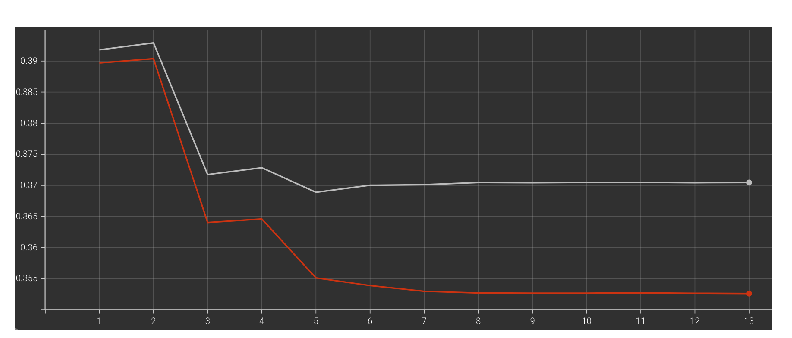
\includegraphics[width=0.7\linewidth]{figures/chapter_V/dnn_loss_curves.pdf}
%     \caption[Loss curves of the signal-extraction discriminant]{%
%         Categorical cross-entropy loss as a function of the training epoch, evaluated on the
%         training (red) and validation (white) subsets.}
%     \label{fig:dnn_loss}
% \end{figure}
%
\begin{figure}[tbp]
    \centering
    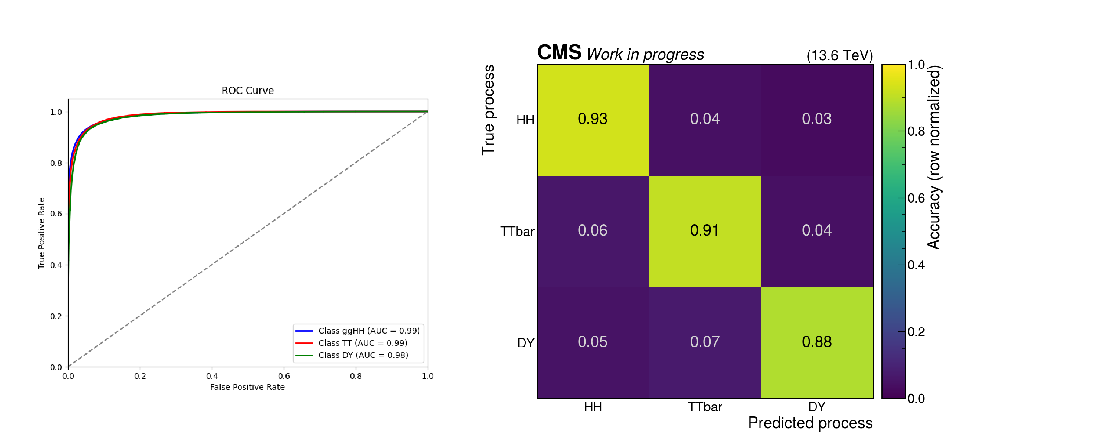
\includegraphics[height=0.385\linewidth, trim=17bp 22bp 316bp 40bp, clip]{figures/chapter_V/dnn_vbf_performance.pdf}\hfill
    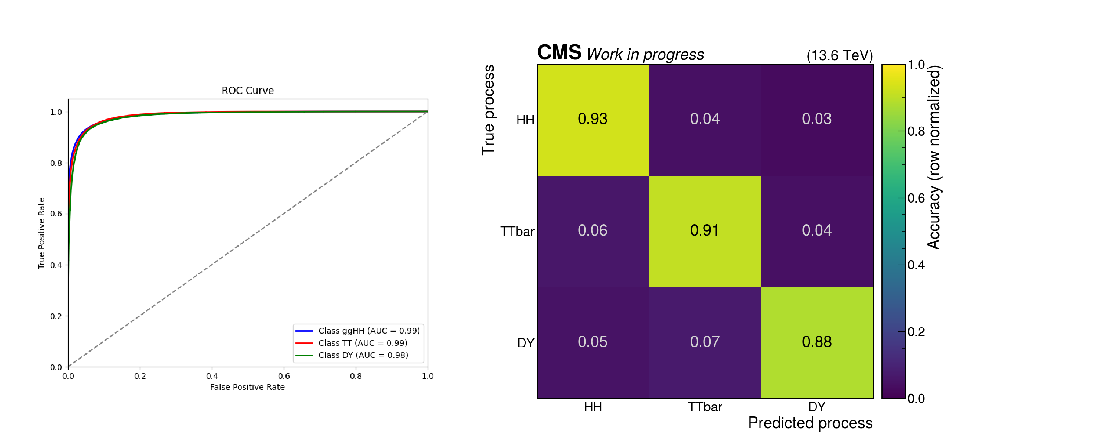
\includegraphics[height=0.385\linewidth, trim=230bp 2bp 72bp 20bp, clip]{figures/chapter_V/dnn_vbf_performance.pdf}
    \caption[Performance of the vector boson fusion discriminant]{%
        ROC curves (left) and confusion matrix normalized by rows (right) of the vector boson
        fusion classifier, evaluated on one of the five subsets; the others yield comparable
        results.}
    \label{fig:dnn_performance}
\end{figure}




Figure \ref{fig:dnn_output} shows the distribution of the $HH$ score for the signal and the main backgrounds in the categories where each classifier is applied, the res2b category for the gluon fusion classifier and the VBF category for the other. The signal concentrates near one, while Drell--Yan and $t\bar{t}$ production accumulate at low values, which motivates the restriction of the fitted range described below.
%
\begin{figure}[tbp]
    \centering
    % TODO: replace with the HH-score distributions
    \fbox{\parbox[c][0.33\linewidth][c]{0.46\linewidth}{\centering ggF classifier, res2b}}\hfill
    \fbox{\parbox[c][0.33\linewidth][c]{0.46\linewidth}{\centering VBF classifier, VBF category}}
    \caption[Distribution of the $HH$ score]{%
        Distribution of the $HH$ score of the gluon fusion classifier in the res2b category
        (left) and of the vector boson fusion classifier in the VBF category (right), for the
        signal and the main backgrounds, normalized to unit area. The dashed line marks the
        lower edge of the fitted range.}
    \label{fig:dnn_output}
\end{figure}


\subsection{Adaptive rebinning}
\label{subsec:bbtt_rebinning}
%
Since the fit is performed on histograms of the $HH$ score, the bin boundaries must be defined. Given that the signal is concentrated in a narrow band near the maximum value, a uniform binning would be a poor choice in this case, as most of the range would contain almost pure background, while the last bin would account for nearly all of the sensitivity. The opposite approach, i.e., finely tuning the binning as much as possible within that narrow band, would also be unhelpful, since the bins would have so few simulated events that predictions within them would be unreliable.

The fitted range is therefore restricted to scores in $[0.75, 1]$, excluding the region where the signal-to-background ratio is too low to inform the signal strength, and the bins within it are built so that the expected signal is distributed approximately uniformly, with no single bin concentrating the sensitivity, while at the same time each bin retains enough simulated events for a reliable prediction. To this end, the distribution is scanned from the highest to the lowest scores, accumulating events until the current bin contains the same fraction of the signal as if it were distributed equally among the planned bins — set at twenty at the outset. This condition flattens the signal distribution and establishes the target bin size. Three further requirements ensure that each bin is usable in the fit.

First, the contributions from Drell--Yan and the $t\bar{t}$ production must be strictly positive, since a process with zero yield in a bin does not allow for relative variations and prevents the treatment of its uncertainties. Second, the statistical uncertainty of the simulated background must not exceed $20\%$, a limit that is relaxed to $30\%$ in the highest-scoring bin, where the signal is more abundant and the statistical requirement would be more detrimental. This condition applies to both the nominal prediction and to each of its systematic variations, so that no bin depends on a poorly populated shifted template. The third condition requires that there be at least ten data events in the template region of the fake factors method, ensuring that the extrapolation described in Section \ref{sec:bbtt_ff} always has a sufficient statistical basis and that its uncertainty does not dominate the bin.

If it is not possible to form twenty bins while adhering to the conditions upon reaching the lower end of the range, the procedure is repeated with one fewer bin until convergence is achieved. The result is a distinct binning for each of the fifty signal regions — ten categories in each of the five data-taking periods — adapted to the separation achieved by the discriminants in each region and to the available statistics.\medskip

The discriminants thus condense into a single observable the information that no variable could capture on its own, ordering the events so that signal and background occupy distinct regions. This defines the distribution against which the fit is performed in each signal region; the statistical treatment of this is described in Section \ref{sec:bbtt_statistics}.
\bigskip

With this, the prediction of the analysis is fully specified. To avoid biasing the analysis strategy, all these choices were made without examining the data in the bins of the discriminants where the signal is concentrated, which remained hidden, or \textit{blinded}, throughout the development of the analysis. The next chapter compares the prediction with the data and translates the comparison into the interpretable results, meaning the strenght with which the signal appears in the data and the significance that can be attributed to it; the limits that arise if it is not observed; and into constraints on the Higgs boson couplings, combining the measurement with the one obtained from the Run 2 dataset.






